\documentclass[twoside]{book}

% Packages required by doxygen
\usepackage{fixltx2e}
\usepackage{calc}
\usepackage{doxygen}
\usepackage[export]{adjustbox} % also loads graphicx
\usepackage{graphicx}
\usepackage[utf8]{inputenc}
\usepackage{makeidx}
\usepackage{multicol}
\usepackage{multirow}
\PassOptionsToPackage{warn}{textcomp}
\usepackage{textcomp}
\usepackage[nointegrals]{wasysym}
\usepackage[table]{xcolor}

% Font selection
\usepackage[T1]{fontenc}
\usepackage[scaled=.90]{helvet}
\usepackage{courier}
\usepackage{amssymb}
\usepackage{sectsty}
\renewcommand{\familydefault}{\sfdefault}
\allsectionsfont{%
  \fontseries{bc}\selectfont%
  \color{darkgray}%
}
\renewcommand{\DoxyLabelFont}{%
  \fontseries{bc}\selectfont%
  \color{darkgray}%
}
\newcommand{\+}{\discretionary{\mbox{\scriptsize$\hookleftarrow$}}{}{}}

% Page & text layout
\usepackage{geometry}
\geometry{%
  a4paper,%
  top=2.5cm,%
  bottom=2.5cm,%
  left=2.5cm,%
  right=2.5cm%
}
\tolerance=750
\hfuzz=15pt
\hbadness=750
\setlength{\emergencystretch}{15pt}
\setlength{\parindent}{0cm}
\setlength{\parskip}{3ex plus 2ex minus 2ex}
\makeatletter
\renewcommand{\paragraph}{%
  \@startsection{paragraph}{4}{0ex}{-1.0ex}{1.0ex}{%
    \normalfont\normalsize\bfseries\SS@parafont%
  }%
}
\renewcommand{\subparagraph}{%
  \@startsection{subparagraph}{5}{0ex}{-1.0ex}{1.0ex}{%
    \normalfont\normalsize\bfseries\SS@subparafont%
  }%
}
\makeatother

% Headers & footers
\usepackage{fancyhdr}
\pagestyle{fancyplain}
\fancyhead[LE]{\fancyplain{}{\bfseries\thepage}}
\fancyhead[CE]{\fancyplain{}{}}
\fancyhead[RE]{\fancyplain{}{\bfseries\leftmark}}
\fancyhead[LO]{\fancyplain{}{\bfseries\rightmark}}
\fancyhead[CO]{\fancyplain{}{}}
\fancyhead[RO]{\fancyplain{}{\bfseries\thepage}}
\fancyfoot[LE]{\fancyplain{}{}}
\fancyfoot[CE]{\fancyplain{}{}}
\fancyfoot[RE]{\fancyplain{}{\bfseries\scriptsize Generated by Doxygen }}
\fancyfoot[LO]{\fancyplain{}{\bfseries\scriptsize Generated by Doxygen }}
\fancyfoot[CO]{\fancyplain{}{}}
\fancyfoot[RO]{\fancyplain{}{}}
\renewcommand{\footrulewidth}{0.4pt}
\renewcommand{\chaptermark}[1]{%
  \markboth{#1}{}%
}
\renewcommand{\sectionmark}[1]{%
  \markright{\thesection\ #1}%
}

% Indices & bibliography
\usepackage{natbib}
\usepackage[titles]{tocloft}
\setcounter{tocdepth}{3}
\setcounter{secnumdepth}{5}
\makeindex

% Hyperlinks (required, but should be loaded last)
\usepackage{ifpdf}
\ifpdf
  \usepackage[pdftex,pagebackref=true]{hyperref}
\else
  \usepackage[ps2pdf,pagebackref=true]{hyperref}
\fi
\hypersetup{%
  colorlinks=true,%
  linkcolor=blue,%
  citecolor=blue,%
  unicode%
}

% Custom commands
\newcommand{\clearemptydoublepage}{%
  \newpage{\pagestyle{empty}\cleardoublepage}%
}

\usepackage{caption}
\captionsetup{labelsep=space,justification=centering,font={bf},singlelinecheck=off,skip=4pt,position=top}

%===== C O N T E N T S =====

\begin{document}

% Titlepage & ToC
\hypersetup{pageanchor=false,
             bookmarksnumbered=true,
             pdfencoding=unicode
            }
\pagenumbering{alph}
\begin{titlepage}
\vspace*{7cm}
\begin{center}%
{\Large Game Engine }\\
\vspace*{1cm}
{\large Generated by Doxygen 1.8.14}\\
\end{center}
\end{titlepage}
\clearemptydoublepage
\pagenumbering{roman}
\tableofcontents
\clearemptydoublepage
\pagenumbering{arabic}
\hypersetup{pageanchor=true}

%--- Begin generated contents ---
\chapter{Hierarchical Index}
\section{Class Hierarchy}
This inheritance list is sorted roughly, but not completely, alphabetically\+:\begin{DoxyCompactList}
\item \contentsline{section}{Box\+Collision}{\pageref{class_box_collision}}{}
\item \contentsline{section}{Component}{\pageref{class_component}}{}
\begin{DoxyCompactList}
\item \contentsline{section}{Button}{\pageref{class_button}}{}
\item \contentsline{section}{Camera}{\pageref{class_camera}}{}
\item \contentsline{section}{Material}{\pageref{class_material}}{}
\item \contentsline{section}{Mesh\+Renderer}{\pageref{class_mesh_renderer}}{}
\begin{DoxyCompactList}
\item \contentsline{section}{Orthagraphic}{\pageref{class_orthagraphic}}{}
\end{DoxyCompactList}
\item \contentsline{section}{Transform}{\pageref{class_transform}}{}
\end{DoxyCompactList}
\item \contentsline{section}{Core}{\pageref{class_core}}{}
\item \contentsline{section}{Entity}{\pageref{class_entity}}{}
\item \contentsline{section}{Environment}{\pageref{class_environment}}{}
\item exception\begin{DoxyCompactList}
\item \contentsline{section}{Exception}{\pageref{class_exception}}{}
\end{DoxyCompactList}
\item \contentsline{section}{Game\+Object}{\pageref{class_game_object}}{}
\item \contentsline{section}{Keyboard\+Handler}{\pageref{class_keyboard_handler}}{}
\item \contentsline{section}{Mat\+Resource}{\pageref{struct_mat_resource}}{}
\item \contentsline{section}{Mesh\+Resource}{\pageref{struct_mesh_resource}}{}
\item \contentsline{section}{Mouse\+Handler}{\pageref{class_mouse_handler}}{}
\item \contentsline{section}{Resources}{\pageref{class_resources}}{}
\item \contentsline{section}{Screen}{\pageref{class_screen}}{}
\item \contentsline{section}{Shader\+Program}{\pageref{class_shader_program}}{}
\item \contentsline{section}{Sound}{\pageref{class_sound}}{}
\item \contentsline{section}{Sound\+Init}{\pageref{struct_sound_init}}{}
\item \contentsline{section}{stbi\+\_\+io\+\_\+callbacks}{\pageref{structstbi__io__callbacks}}{}
\item \contentsline{section}{Vertex\+Array}{\pageref{class_vertex_array}}{}
\item \contentsline{section}{Vertex\+Buffer}{\pageref{class_vertex_buffer}}{}
\end{DoxyCompactList}

\chapter{Class Index}
\section{Class List}
Here are the classes, structs, unions and interfaces with brief descriptions\+:\begin{DoxyCompactList}
\item\contentsline{section}{\mbox{\hyperlink{class_box_collision}{Box\+Collision}} }{\pageref{class_box_collision}}{}
\item\contentsline{section}{\mbox{\hyperlink{class_button}{Button}} }{\pageref{class_button}}{}
\item\contentsline{section}{\mbox{\hyperlink{class_camera}{Camera}} }{\pageref{class_camera}}{}
\item\contentsline{section}{\mbox{\hyperlink{class_component}{Component}} }{\pageref{class_component}}{}
\item\contentsline{section}{\mbox{\hyperlink{class_core}{Core}} }{\pageref{class_core}}{}
\item\contentsline{section}{\mbox{\hyperlink{class_entity}{Entity}} }{\pageref{class_entity}}{}
\item\contentsline{section}{\mbox{\hyperlink{class_environment}{Environment}} }{\pageref{class_environment}}{}
\item\contentsline{section}{\mbox{\hyperlink{class_exception}{Exception}} }{\pageref{class_exception}}{}
\item\contentsline{section}{\mbox{\hyperlink{class_game_object}{Game\+Object}} }{\pageref{class_game_object}}{}
\item\contentsline{section}{\mbox{\hyperlink{class_keyboard_handler}{Keyboard\+Handler}} }{\pageref{class_keyboard_handler}}{}
\item\contentsline{section}{\mbox{\hyperlink{class_material}{Material}} }{\pageref{class_material}}{}
\item\contentsline{section}{\mbox{\hyperlink{struct_mat_resource}{Mat\+Resource}} }{\pageref{struct_mat_resource}}{}
\item\contentsline{section}{\mbox{\hyperlink{class_mesh_renderer}{Mesh\+Renderer}} }{\pageref{class_mesh_renderer}}{}
\item\contentsline{section}{\mbox{\hyperlink{struct_mesh_resource}{Mesh\+Resource}} }{\pageref{struct_mesh_resource}}{}
\item\contentsline{section}{\mbox{\hyperlink{class_mouse_handler}{Mouse\+Handler}} }{\pageref{class_mouse_handler}}{}
\item\contentsline{section}{\mbox{\hyperlink{class_orthagraphic}{Orthagraphic}} }{\pageref{class_orthagraphic}}{}
\item\contentsline{section}{\mbox{\hyperlink{class_resources}{Resources}} }{\pageref{class_resources}}{}
\item\contentsline{section}{\mbox{\hyperlink{class_screen}{Screen}} }{\pageref{class_screen}}{}
\item\contentsline{section}{\mbox{\hyperlink{class_shader_program}{Shader\+Program}} }{\pageref{class_shader_program}}{}
\item\contentsline{section}{\mbox{\hyperlink{class_sound}{Sound}} }{\pageref{class_sound}}{}
\item\contentsline{section}{\mbox{\hyperlink{struct_sound_init}{Sound\+Init}} }{\pageref{struct_sound_init}}{}
\item\contentsline{section}{\mbox{\hyperlink{structstbi__io__callbacks}{stbi\+\_\+io\+\_\+callbacks}} }{\pageref{structstbi__io__callbacks}}{}
\item\contentsline{section}{\mbox{\hyperlink{class_transform}{Transform}} }{\pageref{class_transform}}{}
\item\contentsline{section}{\mbox{\hyperlink{class_vertex_array}{Vertex\+Array}} }{\pageref{class_vertex_array}}{}
\item\contentsline{section}{\mbox{\hyperlink{class_vertex_buffer}{Vertex\+Buffer}} }{\pageref{class_vertex_buffer}}{}
\end{DoxyCompactList}

\chapter{File Index}
\section{File List}
Here is a list of all files with brief descriptions\+:\begin{DoxyCompactList}
\item\contentsline{section}{\mbox{\hyperlink{_box_collision_8cpp}{Box\+Collision.\+cpp}} }{\pageref{_box_collision_8cpp}}{}
\item\contentsline{section}{\mbox{\hyperlink{_box_collision_8h}{Box\+Collision.\+h}} }{\pageref{_box_collision_8h}}{}
\item\contentsline{section}{\mbox{\hyperlink{_button_8cpp}{Button.\+cpp}} }{\pageref{_button_8cpp}}{}
\item\contentsline{section}{\mbox{\hyperlink{_button_8h}{Button.\+h}} }{\pageref{_button_8h}}{}
\item\contentsline{section}{\mbox{\hyperlink{_camera_8cpp}{Camera.\+cpp}} }{\pageref{_camera_8cpp}}{}
\item\contentsline{section}{\mbox{\hyperlink{_camera_8h}{Camera.\+h}} }{\pageref{_camera_8h}}{}
\item\contentsline{section}{\mbox{\hyperlink{_component_8cpp}{Component.\+cpp}} }{\pageref{_component_8cpp}}{}
\item\contentsline{section}{\mbox{\hyperlink{_component_8h}{Component.\+h}} }{\pageref{_component_8h}}{}
\item\contentsline{section}{\mbox{\hyperlink{_core_8cpp}{Core.\+cpp}} }{\pageref{_core_8cpp}}{}
\item\contentsline{section}{\mbox{\hyperlink{_core_8h}{Core.\+h}} }{\pageref{_core_8h}}{}
\item\contentsline{section}{\mbox{\hyperlink{_entity_8cpp}{Entity.\+cpp}} }{\pageref{_entity_8cpp}}{}
\item\contentsline{section}{\mbox{\hyperlink{_entity_8h}{Entity.\+h}} }{\pageref{_entity_8h}}{}
\item\contentsline{section}{\mbox{\hyperlink{_environment_8cpp}{Environment.\+cpp}} }{\pageref{_environment_8cpp}}{}
\item\contentsline{section}{\mbox{\hyperlink{_environment_8h}{Environment.\+h}} }{\pageref{_environment_8h}}{}
\item\contentsline{section}{\mbox{\hyperlink{_exception_8cpp}{Exception.\+cpp}} }{\pageref{_exception_8cpp}}{}
\item\contentsline{section}{\mbox{\hyperlink{_exception_8h}{Exception.\+h}} }{\pageref{_exception_8h}}{}
\item\contentsline{section}{\mbox{\hyperlink{_game_engine_8cpp}{Game\+Engine.\+cpp}} }{\pageref{_game_engine_8cpp}}{}
\item\contentsline{section}{\mbox{\hyperlink{_game_engine_8h}{Game\+Engine.\+h}} }{\pageref{_game_engine_8h}}{}
\item\contentsline{section}{\mbox{\hyperlink{_keyboard_handler_8cpp}{Keyboard\+Handler.\+cpp}} }{\pageref{_keyboard_handler_8cpp}}{}
\item\contentsline{section}{\mbox{\hyperlink{_keyboard_handler_8h}{Keyboard\+Handler.\+h}} }{\pageref{_keyboard_handler_8h}}{}
\item\contentsline{section}{\mbox{\hyperlink{_material_8cpp}{Material.\+cpp}} }{\pageref{_material_8cpp}}{}
\item\contentsline{section}{\mbox{\hyperlink{_material_8h}{Material.\+h}} }{\pageref{_material_8h}}{}
\item\contentsline{section}{\mbox{\hyperlink{_mesh_renderer_8cpp}{Mesh\+Renderer.\+cpp}} }{\pageref{_mesh_renderer_8cpp}}{}
\item\contentsline{section}{\mbox{\hyperlink{_mesh_renderer_8h}{Mesh\+Renderer.\+h}} }{\pageref{_mesh_renderer_8h}}{}
\item\contentsline{section}{\mbox{\hyperlink{_mouse_handler_8cpp}{Mouse\+Handler.\+cpp}} }{\pageref{_mouse_handler_8cpp}}{}
\item\contentsline{section}{\mbox{\hyperlink{_mouse_handler_8h}{Mouse\+Handler.\+h}} }{\pageref{_mouse_handler_8h}}{}
\item\contentsline{section}{\mbox{\hyperlink{_orthagraphic_8cpp}{Orthagraphic.\+cpp}} }{\pageref{_orthagraphic_8cpp}}{}
\item\contentsline{section}{\mbox{\hyperlink{_orthagraphic_8h}{Orthagraphic.\+h}} }{\pageref{_orthagraphic_8h}}{}
\item\contentsline{section}{\mbox{\hyperlink{_resources_8cpp}{Resources.\+cpp}} }{\pageref{_resources_8cpp}}{}
\item\contentsline{section}{\mbox{\hyperlink{_resources_8h}{Resources.\+h}} }{\pageref{_resources_8h}}{}
\item\contentsline{section}{\mbox{\hyperlink{_screen_8cpp}{Screen.\+cpp}} }{\pageref{_screen_8cpp}}{}
\item\contentsline{section}{\mbox{\hyperlink{_screen_8h}{Screen.\+h}} }{\pageref{_screen_8h}}{}
\item\contentsline{section}{\mbox{\hyperlink{_shader_program_8cpp}{Shader\+Program.\+cpp}} }{\pageref{_shader_program_8cpp}}{}
\item\contentsline{section}{\mbox{\hyperlink{_shader_program_8h}{Shader\+Program.\+h}} }{\pageref{_shader_program_8h}}{}
\item\contentsline{section}{\mbox{\hyperlink{_sound_8cpp}{Sound.\+cpp}} }{\pageref{_sound_8cpp}}{}
\item\contentsline{section}{\mbox{\hyperlink{_sound_8h}{Sound.\+h}} }{\pageref{_sound_8h}}{}
\item\contentsline{section}{\mbox{\hyperlink{stb__image_8cpp}{stb\+\_\+image.\+cpp}} }{\pageref{stb__image_8cpp}}{}
\item\contentsline{section}{\mbox{\hyperlink{stb__image_8h}{stb\+\_\+image.\+h}} }{\pageref{stb__image_8h}}{}
\item\contentsline{section}{\mbox{\hyperlink{_transform_8cpp}{Transform.\+cpp}} }{\pageref{_transform_8cpp}}{}
\item\contentsline{section}{\mbox{\hyperlink{_transform_8h}{Transform.\+h}} }{\pageref{_transform_8h}}{}
\item\contentsline{section}{\mbox{\hyperlink{_vertex_array_8cpp}{Vertex\+Array.\+cpp}} }{\pageref{_vertex_array_8cpp}}{}
\item\contentsline{section}{\mbox{\hyperlink{_vertex_array_8h}{Vertex\+Array.\+h}} }{\pageref{_vertex_array_8h}}{}
\item\contentsline{section}{\mbox{\hyperlink{_vertex_buffer_8cpp}{Vertex\+Buffer.\+cpp}} }{\pageref{_vertex_buffer_8cpp}}{}
\item\contentsline{section}{\mbox{\hyperlink{_vertex_buffer_8h}{Vertex\+Buffer.\+h}} }{\pageref{_vertex_buffer_8h}}{}
\end{DoxyCompactList}

\chapter{Class Documentation}
\hypertarget{class_box_collision}{}\section{Box\+Collision Class Reference}
\label{class_box_collision}\index{Box\+Collision@{Box\+Collision}}


{\ttfamily \#include $<$Box\+Collision.\+h$>$}



Collaboration diagram for Box\+Collision\+:
\nopagebreak
\begin{figure}[H]
\begin{center}
\leavevmode
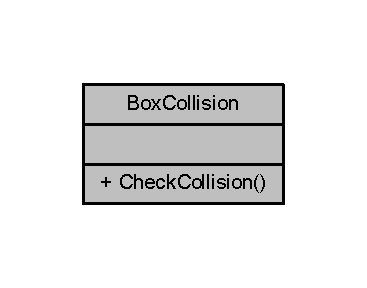
\includegraphics[width=176pt]{class_box_collision__coll__graph}
\end{center}
\end{figure}
\subsection*{Public Member Functions}
\begin{DoxyCompactItemize}
\item 
bool \mbox{\hyperlink{class_box_collision_a2cdd4303a969f89a37054bdc881ad095}{Check\+Collision}} (std\+::weak\+\_\+ptr$<$ \mbox{\hyperlink{class_entity}{Entity}} $>$ \+\_\+a, std\+::weak\+\_\+ptr$<$ \mbox{\hyperlink{class_entity}{Entity}} $>$ \+\_\+b)
\end{DoxyCompactItemize}


\subsection{Member Function Documentation}
\mbox{\Hypertarget{class_box_collision_a2cdd4303a969f89a37054bdc881ad095}\label{class_box_collision_a2cdd4303a969f89a37054bdc881ad095}} 
\index{Box\+Collision@{Box\+Collision}!Check\+Collision@{Check\+Collision}}
\index{Check\+Collision@{Check\+Collision}!Box\+Collision@{Box\+Collision}}
\subsubsection{\texorpdfstring{Check\+Collision()}{CheckCollision()}}
{\footnotesize\ttfamily bool Box\+Collision\+::\+Check\+Collision (\begin{DoxyParamCaption}\item[{std\+::weak\+\_\+ptr$<$ \mbox{\hyperlink{class_entity}{Entity}} $>$}]{\+\_\+a,  }\item[{std\+::weak\+\_\+ptr$<$ \mbox{\hyperlink{class_entity}{Entity}} $>$}]{\+\_\+b }\end{DoxyParamCaption})}



The documentation for this class was generated from the following files\+:\begin{DoxyCompactItemize}
\item 
\mbox{\hyperlink{_box_collision_8h}{Box\+Collision.\+h}}\item 
\mbox{\hyperlink{_box_collision_8cpp}{Box\+Collision.\+cpp}}\end{DoxyCompactItemize}

\hypertarget{class_button}{}\section{Button Class Reference}
\label{class_button}\index{Button@{Button}}


{\ttfamily \#include $<$Button.\+h$>$}



Inheritance diagram for Button\+:
\nopagebreak
\begin{figure}[H]
\begin{center}
\leavevmode
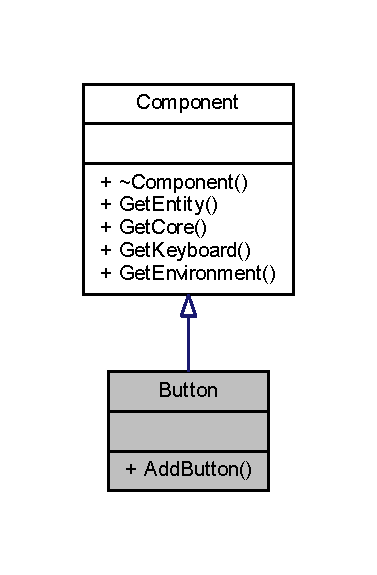
\includegraphics[width=181pt]{class_button__inherit__graph}
\end{center}
\end{figure}


Collaboration diagram for Button\+:
\nopagebreak
\begin{figure}[H]
\begin{center}
\leavevmode
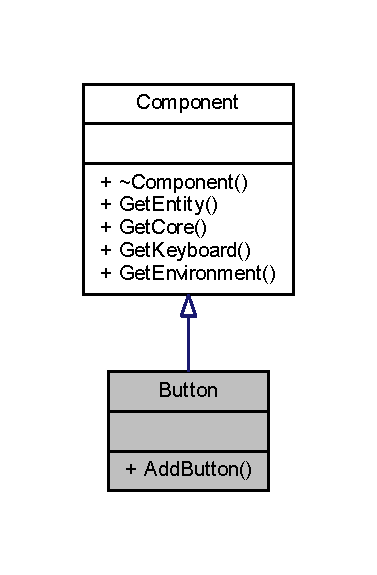
\includegraphics[width=181pt]{class_button__coll__graph}
\end{center}
\end{figure}
\subsection*{Public Member Functions}
\begin{DoxyCompactItemize}
\item 
void \mbox{\hyperlink{class_button_a02344644a142f432e211f2352e40aaa3}{Add\+Button}} (glm\+::vec3 \+\_\+position)
\end{DoxyCompactItemize}


\subsection{Member Function Documentation}
\mbox{\Hypertarget{class_button_a02344644a142f432e211f2352e40aaa3}\label{class_button_a02344644a142f432e211f2352e40aaa3}} 
\index{Button@{Button}!Add\+Button@{Add\+Button}}
\index{Add\+Button@{Add\+Button}!Button@{Button}}
\subsubsection{\texorpdfstring{Add\+Button()}{AddButton()}}
{\footnotesize\ttfamily void Button\+::\+Add\+Button (\begin{DoxyParamCaption}\item[{glm\+::vec3}]{\+\_\+position }\end{DoxyParamCaption})}



The documentation for this class was generated from the following files\+:\begin{DoxyCompactItemize}
\item 
\mbox{\hyperlink{_button_8h}{Button.\+h}}\item 
\mbox{\hyperlink{_button_8cpp}{Button.\+cpp}}\end{DoxyCompactItemize}

\hypertarget{class_camera}{}\section{Camera Class Reference}
\label{class_camera}\index{Camera@{Camera}}


{\ttfamily \#include $<$Camera.\+h$>$}



Inheritance diagram for Camera\+:
\nopagebreak
\begin{figure}[H]
\begin{center}
\leavevmode
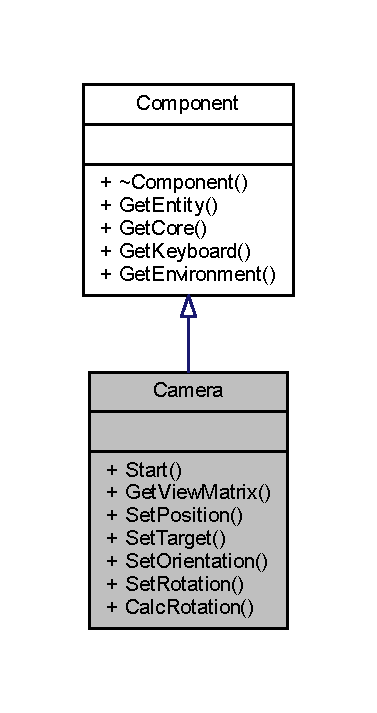
\includegraphics[width=181pt]{class_camera__inherit__graph}
\end{center}
\end{figure}


Collaboration diagram for Camera\+:
\nopagebreak
\begin{figure}[H]
\begin{center}
\leavevmode
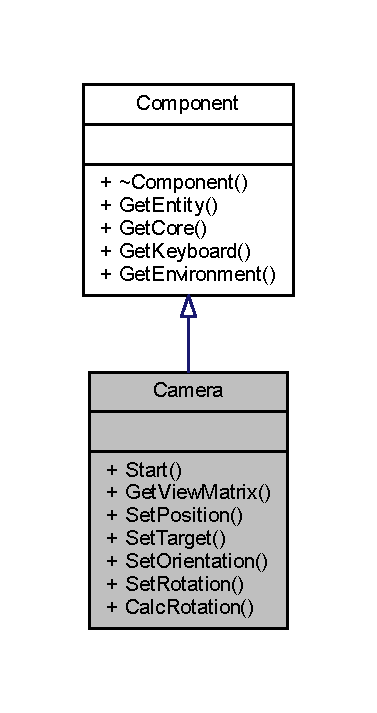
\includegraphics[width=181pt]{class_camera__coll__graph}
\end{center}
\end{figure}
\subsection*{Public Member Functions}
\begin{DoxyCompactItemize}
\item 
void \mbox{\hyperlink{class_camera_aaaf81f5649f2f9e003a922d4abd29c99}{Start}} (glm\+::vec3 \+\_\+position, glm\+::vec3 \+\_\+target, glm\+::vec3 \+\_\+orientation)
\item 
glm\+::mat4 \mbox{\hyperlink{class_camera_affa333055635aed96518c4c66be9a70c}{Get\+View\+Matrix}} ()
\item 
void \mbox{\hyperlink{class_camera_ab2c13ba0cd3d3b08feeab6a4f7d496bc}{Set\+Position}} (glm\+::vec3 \+\_\+position)
\item 
void \mbox{\hyperlink{class_camera_a9073f66c6522efed683d2867e197a6c8}{Set\+Target}} (glm\+::vec3 \+\_\+target)
\item 
void \mbox{\hyperlink{class_camera_a6518b723541de76a710e337a0ee364b0}{Set\+Orientation}} (glm\+::vec3 \+\_\+orientation)
\item 
void \mbox{\hyperlink{class_camera_ae054ebd0fdc18f36dfcd4a3c968ec471}{Set\+Rotation}} (float \+\_\+angle, glm\+::vec3 \+\_\+orientation)
\item 
void \mbox{\hyperlink{class_camera_a3d79803c1dc47d6c1065072a6c5cd8be}{Calc\+Rotation}} ()
\end{DoxyCompactItemize}


\subsection{Member Function Documentation}
\mbox{\Hypertarget{class_camera_a3d79803c1dc47d6c1065072a6c5cd8be}\label{class_camera_a3d79803c1dc47d6c1065072a6c5cd8be}} 
\index{Camera@{Camera}!Calc\+Rotation@{Calc\+Rotation}}
\index{Calc\+Rotation@{Calc\+Rotation}!Camera@{Camera}}
\subsubsection{\texorpdfstring{Calc\+Rotation()}{CalcRotation()}}
{\footnotesize\ttfamily void Camera\+::\+Calc\+Rotation (\begin{DoxyParamCaption}{ }\end{DoxyParamCaption})}

\mbox{\Hypertarget{class_camera_affa333055635aed96518c4c66be9a70c}\label{class_camera_affa333055635aed96518c4c66be9a70c}} 
\index{Camera@{Camera}!Get\+View\+Matrix@{Get\+View\+Matrix}}
\index{Get\+View\+Matrix@{Get\+View\+Matrix}!Camera@{Camera}}
\subsubsection{\texorpdfstring{Get\+View\+Matrix()}{GetViewMatrix()}}
{\footnotesize\ttfamily glm\+::mat4 Camera\+::\+Get\+View\+Matrix (\begin{DoxyParamCaption}{ }\end{DoxyParamCaption})}

\mbox{\Hypertarget{class_camera_a6518b723541de76a710e337a0ee364b0}\label{class_camera_a6518b723541de76a710e337a0ee364b0}} 
\index{Camera@{Camera}!Set\+Orientation@{Set\+Orientation}}
\index{Set\+Orientation@{Set\+Orientation}!Camera@{Camera}}
\subsubsection{\texorpdfstring{Set\+Orientation()}{SetOrientation()}}
{\footnotesize\ttfamily void Camera\+::\+Set\+Orientation (\begin{DoxyParamCaption}\item[{glm\+::vec3}]{\+\_\+orientation }\end{DoxyParamCaption})\hspace{0.3cm}{\ttfamily [inline]}}

\mbox{\Hypertarget{class_camera_ab2c13ba0cd3d3b08feeab6a4f7d496bc}\label{class_camera_ab2c13ba0cd3d3b08feeab6a4f7d496bc}} 
\index{Camera@{Camera}!Set\+Position@{Set\+Position}}
\index{Set\+Position@{Set\+Position}!Camera@{Camera}}
\subsubsection{\texorpdfstring{Set\+Position()}{SetPosition()}}
{\footnotesize\ttfamily void Camera\+::\+Set\+Position (\begin{DoxyParamCaption}\item[{glm\+::vec3}]{\+\_\+position }\end{DoxyParamCaption})}

Here is the call graph for this function\+:
\nopagebreak
\begin{figure}[H]
\begin{center}
\leavevmode
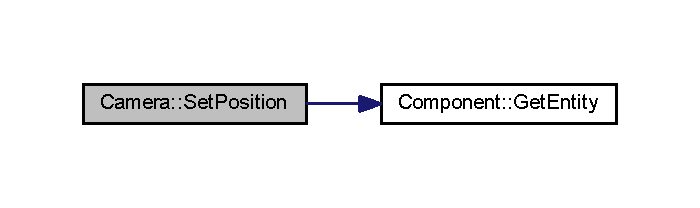
\includegraphics[width=336pt]{class_camera_ab2c13ba0cd3d3b08feeab6a4f7d496bc_cgraph}
\end{center}
\end{figure}
Here is the caller graph for this function\+:
\nopagebreak
\begin{figure}[H]
\begin{center}
\leavevmode
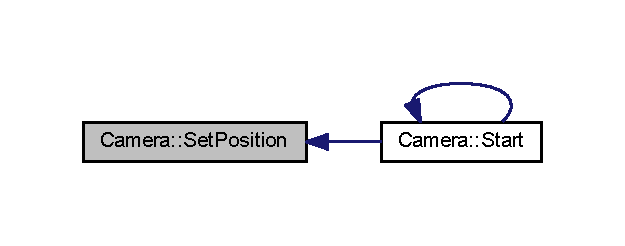
\includegraphics[width=300pt]{class_camera_ab2c13ba0cd3d3b08feeab6a4f7d496bc_icgraph}
\end{center}
\end{figure}
\mbox{\Hypertarget{class_camera_ae054ebd0fdc18f36dfcd4a3c968ec471}\label{class_camera_ae054ebd0fdc18f36dfcd4a3c968ec471}} 
\index{Camera@{Camera}!Set\+Rotation@{Set\+Rotation}}
\index{Set\+Rotation@{Set\+Rotation}!Camera@{Camera}}
\subsubsection{\texorpdfstring{Set\+Rotation()}{SetRotation()}}
{\footnotesize\ttfamily void Camera\+::\+Set\+Rotation (\begin{DoxyParamCaption}\item[{float}]{\+\_\+angle,  }\item[{glm\+::vec3}]{\+\_\+orientation }\end{DoxyParamCaption})}

\mbox{\Hypertarget{class_camera_a9073f66c6522efed683d2867e197a6c8}\label{class_camera_a9073f66c6522efed683d2867e197a6c8}} 
\index{Camera@{Camera}!Set\+Target@{Set\+Target}}
\index{Set\+Target@{Set\+Target}!Camera@{Camera}}
\subsubsection{\texorpdfstring{Set\+Target()}{SetTarget()}}
{\footnotesize\ttfamily void Camera\+::\+Set\+Target (\begin{DoxyParamCaption}\item[{glm\+::vec3}]{\+\_\+target }\end{DoxyParamCaption})\hspace{0.3cm}{\ttfamily [inline]}}

\mbox{\Hypertarget{class_camera_aaaf81f5649f2f9e003a922d4abd29c99}\label{class_camera_aaaf81f5649f2f9e003a922d4abd29c99}} 
\index{Camera@{Camera}!Start@{Start}}
\index{Start@{Start}!Camera@{Camera}}
\subsubsection{\texorpdfstring{Start()}{Start()}}
{\footnotesize\ttfamily void Camera\+::\+Start (\begin{DoxyParamCaption}\item[{glm\+::vec3}]{\+\_\+position,  }\item[{glm\+::vec3}]{\+\_\+target,  }\item[{glm\+::vec3}]{\+\_\+orientation }\end{DoxyParamCaption})}

Here is the call graph for this function\+:
\nopagebreak
\begin{figure}[H]
\begin{center}
\leavevmode
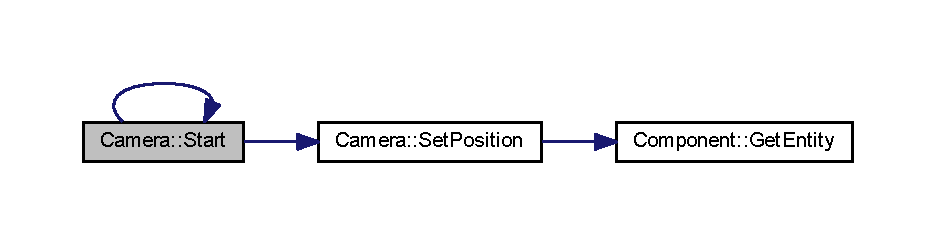
\includegraphics[width=350pt]{class_camera_aaaf81f5649f2f9e003a922d4abd29c99_cgraph}
\end{center}
\end{figure}
Here is the caller graph for this function\+:
\nopagebreak
\begin{figure}[H]
\begin{center}
\leavevmode
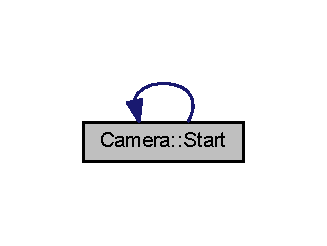
\includegraphics[width=157pt]{class_camera_aaaf81f5649f2f9e003a922d4abd29c99_icgraph}
\end{center}
\end{figure}


The documentation for this class was generated from the following files\+:\begin{DoxyCompactItemize}
\item 
\mbox{\hyperlink{_camera_8h}{Camera.\+h}}\item 
\mbox{\hyperlink{_camera_8cpp}{Camera.\+cpp}}\end{DoxyCompactItemize}

\hypertarget{class_component}{}\section{Component Class Reference}
\label{class_component}\index{Component@{Component}}


{\ttfamily \#include $<$Component.\+h$>$}



Inheritance diagram for Component\+:
\nopagebreak
\begin{figure}[H]
\begin{center}
\leavevmode
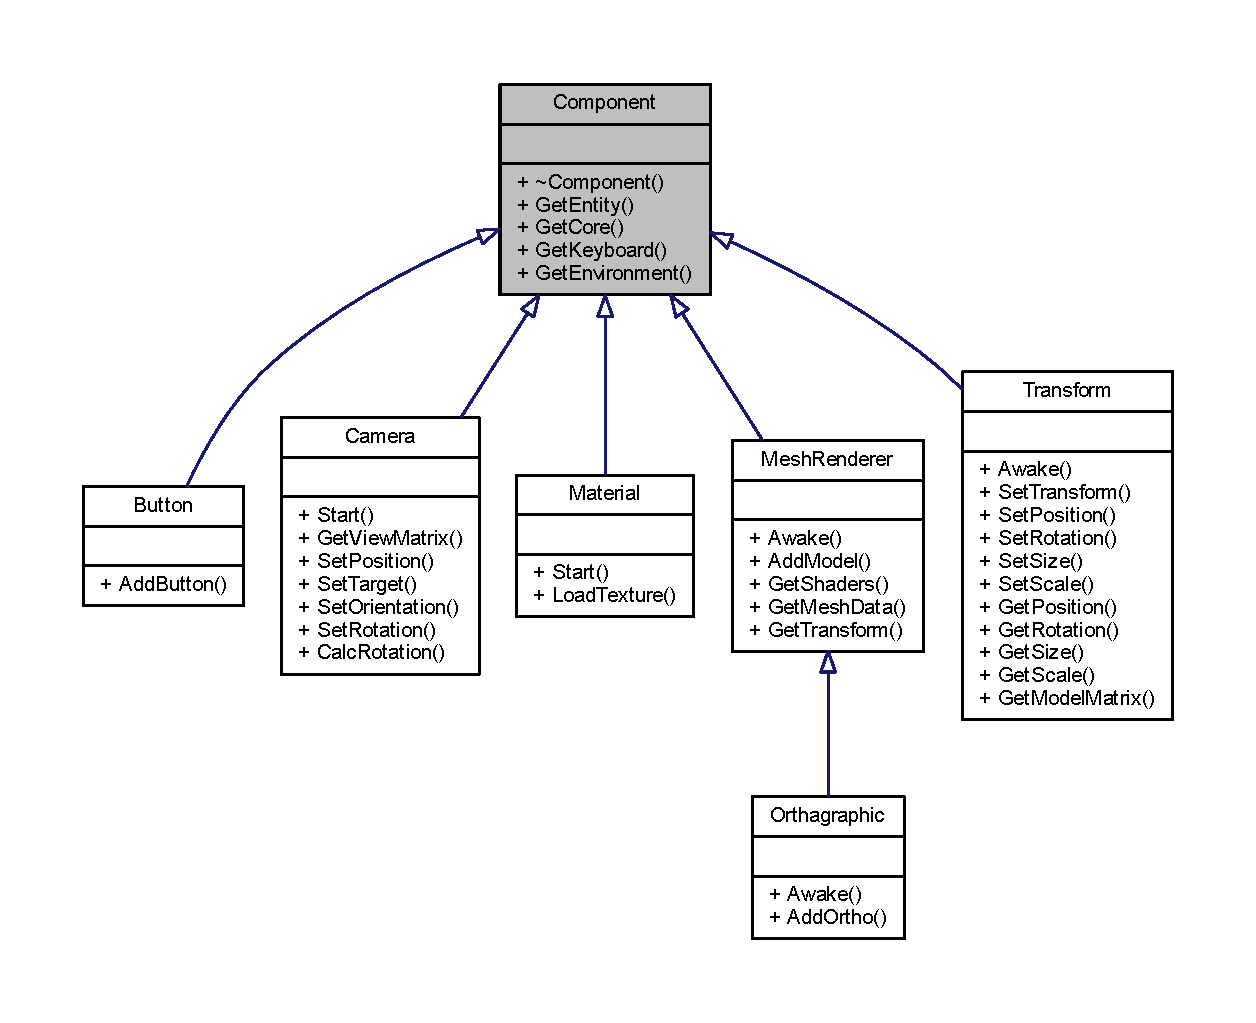
\includegraphics[width=350pt]{class_component__inherit__graph}
\end{center}
\end{figure}


Collaboration diagram for Component\+:
\nopagebreak
\begin{figure}[H]
\begin{center}
\leavevmode
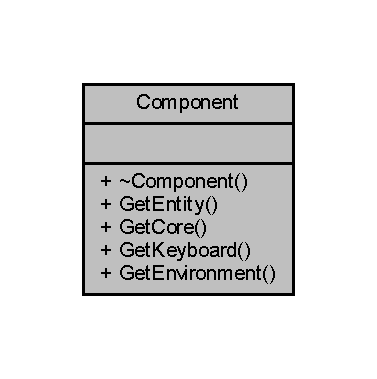
\includegraphics[width=181pt]{class_component__coll__graph}
\end{center}
\end{figure}
\subsection*{Public Member Functions}
\begin{DoxyCompactItemize}
\item 
virtual \mbox{\hyperlink{class_component_ab8378fa275af98e568a7e91d33d867af}{$\sim$\+Component}} ()
\item 
std\+::shared\+\_\+ptr$<$ \mbox{\hyperlink{class_entity}{Entity}} $>$ \mbox{\hyperlink{class_component_a746298ddfd39da5b191926aa8d8f6d95}{Get\+Entity}} ()
\item 
std\+::shared\+\_\+ptr$<$ \mbox{\hyperlink{class_core}{Core}} $>$ \mbox{\hyperlink{class_component_a601ec93559ca1dd75c2c1ea13510594d}{Get\+Core}} ()
\item 
std\+::shared\+\_\+ptr$<$ \mbox{\hyperlink{class_keyboard_handler}{Keyboard\+Handler}} $>$ \mbox{\hyperlink{class_component_a1639a645d23caae1be3b952b850a65c4}{Get\+Keyboard}} ()
\item 
std\+::shared\+\_\+ptr$<$ \mbox{\hyperlink{class_environment}{Environment}} $>$ \mbox{\hyperlink{class_component_acc728e71f991a200996b9215b4b4739a}{Get\+Environment}} ()
\end{DoxyCompactItemize}
\subsection*{Friends}
\begin{DoxyCompactItemize}
\item 
class \mbox{\hyperlink{class_component_a614439ccac0344926adc4c0165d64060}{Entity}}
\end{DoxyCompactItemize}


\subsection{Constructor \& Destructor Documentation}
\mbox{\Hypertarget{class_component_ab8378fa275af98e568a7e91d33d867af}\label{class_component_ab8378fa275af98e568a7e91d33d867af}} 
\index{Component@{Component}!````~Component@{$\sim$\+Component}}
\index{````~Component@{$\sim$\+Component}!Component@{Component}}
\subsubsection{\texorpdfstring{$\sim$\+Component()}{~Component()}}
{\footnotesize\ttfamily Component\+::$\sim$\+Component (\begin{DoxyParamCaption}{ }\end{DoxyParamCaption})\hspace{0.3cm}{\ttfamily [virtual]}}



\subsection{Member Function Documentation}
\mbox{\Hypertarget{class_component_a601ec93559ca1dd75c2c1ea13510594d}\label{class_component_a601ec93559ca1dd75c2c1ea13510594d}} 
\index{Component@{Component}!Get\+Core@{Get\+Core}}
\index{Get\+Core@{Get\+Core}!Component@{Component}}
\subsubsection{\texorpdfstring{Get\+Core()}{GetCore()}}
{\footnotesize\ttfamily std\+::shared\+\_\+ptr$<$ \mbox{\hyperlink{class_core}{Core}} $>$ Component\+::\+Get\+Core (\begin{DoxyParamCaption}{ }\end{DoxyParamCaption})}

Here is the call graph for this function\+:
\nopagebreak
\begin{figure}[H]
\begin{center}
\leavevmode
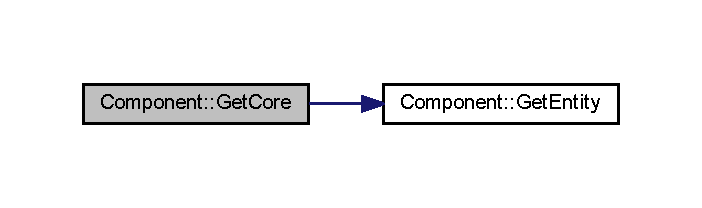
\includegraphics[width=337pt]{class_component_a601ec93559ca1dd75c2c1ea13510594d_cgraph}
\end{center}
\end{figure}
Here is the caller graph for this function\+:
\nopagebreak
\begin{figure}[H]
\begin{center}
\leavevmode
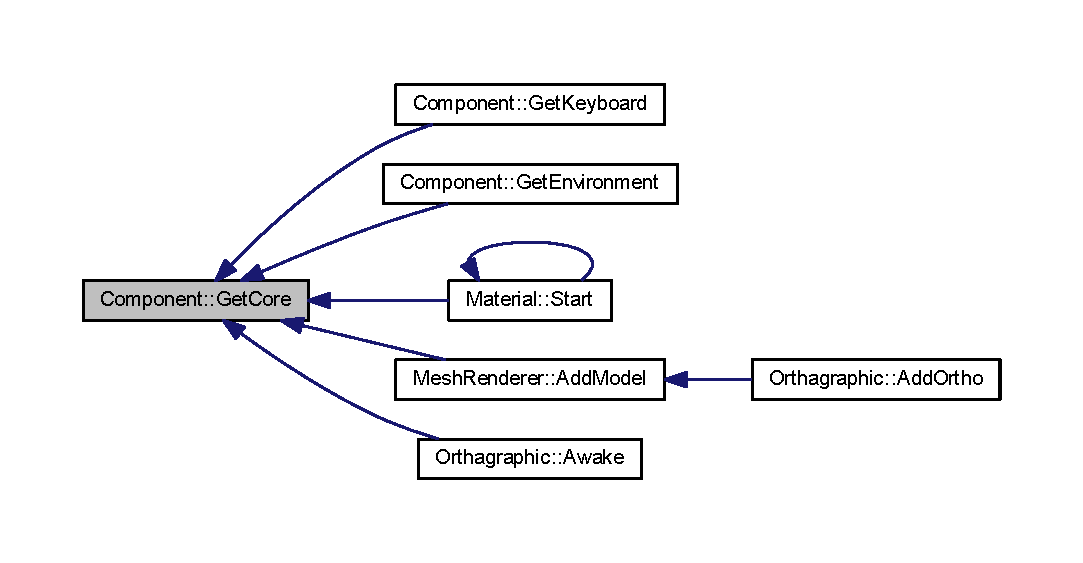
\includegraphics[width=350pt]{class_component_a601ec93559ca1dd75c2c1ea13510594d_icgraph}
\end{center}
\end{figure}
\mbox{\Hypertarget{class_component_a746298ddfd39da5b191926aa8d8f6d95}\label{class_component_a746298ddfd39da5b191926aa8d8f6d95}} 
\index{Component@{Component}!Get\+Entity@{Get\+Entity}}
\index{Get\+Entity@{Get\+Entity}!Component@{Component}}
\subsubsection{\texorpdfstring{Get\+Entity()}{GetEntity()}}
{\footnotesize\ttfamily std\+::shared\+\_\+ptr$<$ \mbox{\hyperlink{class_entity}{Entity}} $>$ Component\+::\+Get\+Entity (\begin{DoxyParamCaption}{ }\end{DoxyParamCaption})}

Here is the caller graph for this function\+:
\nopagebreak
\begin{figure}[H]
\begin{center}
\leavevmode
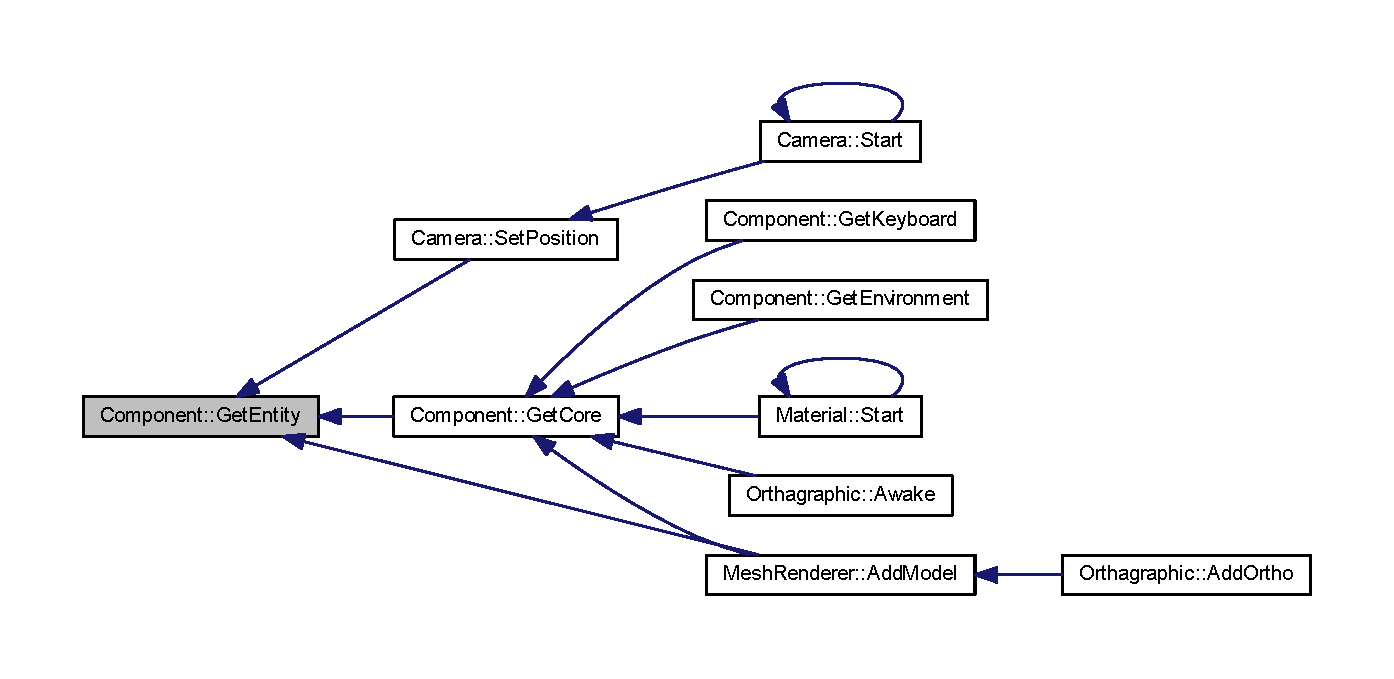
\includegraphics[width=350pt]{class_component_a746298ddfd39da5b191926aa8d8f6d95_icgraph}
\end{center}
\end{figure}
\mbox{\Hypertarget{class_component_acc728e71f991a200996b9215b4b4739a}\label{class_component_acc728e71f991a200996b9215b4b4739a}} 
\index{Component@{Component}!Get\+Environment@{Get\+Environment}}
\index{Get\+Environment@{Get\+Environment}!Component@{Component}}
\subsubsection{\texorpdfstring{Get\+Environment()}{GetEnvironment()}}
{\footnotesize\ttfamily std\+::shared\+\_\+ptr$<$ \mbox{\hyperlink{class_environment}{Environment}} $>$ Component\+::\+Get\+Environment (\begin{DoxyParamCaption}{ }\end{DoxyParamCaption})}

Here is the call graph for this function\+:
\nopagebreak
\begin{figure}[H]
\begin{center}
\leavevmode
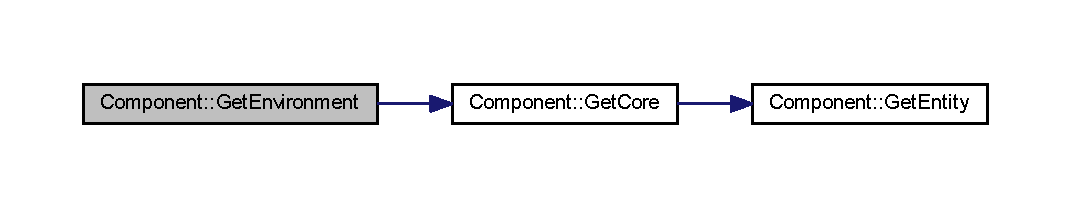
\includegraphics[width=350pt]{class_component_acc728e71f991a200996b9215b4b4739a_cgraph}
\end{center}
\end{figure}
\mbox{\Hypertarget{class_component_a1639a645d23caae1be3b952b850a65c4}\label{class_component_a1639a645d23caae1be3b952b850a65c4}} 
\index{Component@{Component}!Get\+Keyboard@{Get\+Keyboard}}
\index{Get\+Keyboard@{Get\+Keyboard}!Component@{Component}}
\subsubsection{\texorpdfstring{Get\+Keyboard()}{GetKeyboard()}}
{\footnotesize\ttfamily std\+::shared\+\_\+ptr$<$ \mbox{\hyperlink{class_keyboard_handler}{Keyboard\+Handler}} $>$ Component\+::\+Get\+Keyboard (\begin{DoxyParamCaption}{ }\end{DoxyParamCaption})}

Here is the call graph for this function\+:
\nopagebreak
\begin{figure}[H]
\begin{center}
\leavevmode
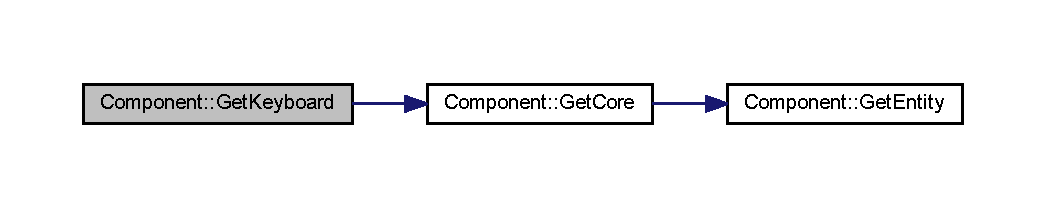
\includegraphics[width=350pt]{class_component_a1639a645d23caae1be3b952b850a65c4_cgraph}
\end{center}
\end{figure}


\subsection{Friends And Related Function Documentation}
\mbox{\Hypertarget{class_component_a614439ccac0344926adc4c0165d64060}\label{class_component_a614439ccac0344926adc4c0165d64060}} 
\index{Component@{Component}!Entity@{Entity}}
\index{Entity@{Entity}!Component@{Component}}
\subsubsection{\texorpdfstring{Entity}{Entity}}
{\footnotesize\ttfamily friend class \mbox{\hyperlink{class_entity}{Entity}}\hspace{0.3cm}{\ttfamily [friend]}}



The documentation for this class was generated from the following files\+:\begin{DoxyCompactItemize}
\item 
\mbox{\hyperlink{_component_8h}{Component.\+h}}\item 
\mbox{\hyperlink{_component_8cpp}{Component.\+cpp}}\end{DoxyCompactItemize}

\hypertarget{class_core}{}\section{Core Class Reference}
\label{class_core}\index{Core@{Core}}


{\ttfamily \#include $<$Core.\+h$>$}



Collaboration diagram for Core\+:
\nopagebreak
\begin{figure}[H]
\begin{center}
\leavevmode
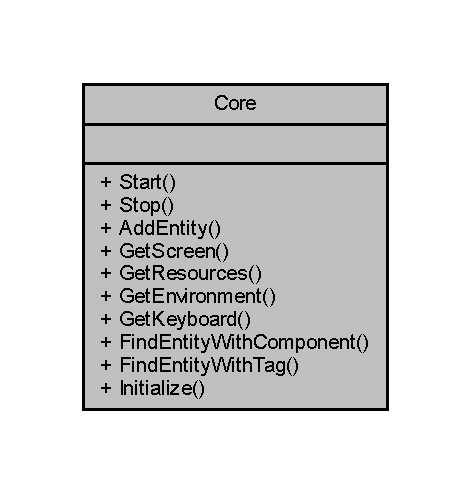
\includegraphics[width=226pt]{class_core__coll__graph}
\end{center}
\end{figure}
\subsection*{Public Member Functions}
\begin{DoxyCompactItemize}
\item 
void \mbox{\hyperlink{class_core_a44f0db8bca5b6fd85f3948250287bdbd}{Start}} ()
\item 
void \mbox{\hyperlink{class_core_acab57c44acf4231e8310d93310667990}{Stop}} ()
\item 
std\+::shared\+\_\+ptr$<$ \mbox{\hyperlink{class_entity}{Entity}} $>$ \mbox{\hyperlink{class_core_a6cd7b26cd56b4a42da9ae8826de0df17}{Add\+Entity}} ()
\item 
std\+::shared\+\_\+ptr$<$ \mbox{\hyperlink{class_screen}{Screen}} $>$ \mbox{\hyperlink{class_core_a76fb4db2f5c8214d1b021bc86b2c3b9c}{Get\+Screen}} ()
\item 
std\+::shared\+\_\+ptr$<$ \mbox{\hyperlink{class_resources}{Resources}} $>$ \mbox{\hyperlink{class_core_acb593d32db59735a95768084eb4f0b19}{Get\+Resources}} ()
\item 
std\+::shared\+\_\+ptr$<$ \mbox{\hyperlink{class_environment}{Environment}} $>$ \mbox{\hyperlink{class_core_a3a17d61ebebe3ebef9dc494f3112e3e7}{Get\+Environment}} ()
\item 
std\+::shared\+\_\+ptr$<$ \mbox{\hyperlink{class_keyboard_handler}{Keyboard\+Handler}} $>$ \mbox{\hyperlink{class_core_a24a4ef158caf9f6a718dd0931e000e6c}{Get\+Keyboard}} ()
\item 
{\footnotesize template$<$typename T $>$ }\\std\+::shared\+\_\+ptr$<$ \mbox{\hyperlink{class_entity}{Entity}} $>$ \mbox{\hyperlink{class_core_a29fd512c6fae721c491de2b1bfcd9ce1}{Find\+Entity\+With\+Component}} ()
\item 
std\+::shared\+\_\+ptr$<$ \mbox{\hyperlink{class_entity}{Entity}} $>$ \mbox{\hyperlink{class_core_a57ad2a53d1d291949c31a6c9ba493cdb}{Find\+Entity\+With\+Tag}} (std\+::string \+\_\+tag)
\end{DoxyCompactItemize}
\subsection*{Static Public Member Functions}
\begin{DoxyCompactItemize}
\item 
static std\+::shared\+\_\+ptr$<$ \mbox{\hyperlink{class_core}{Core}} $>$ \mbox{\hyperlink{class_core_ab62f686765accb870bbde07184b52bef}{Initialize}} ()
\end{DoxyCompactItemize}


\subsection{Member Function Documentation}
\mbox{\Hypertarget{class_core_a6cd7b26cd56b4a42da9ae8826de0df17}\label{class_core_a6cd7b26cd56b4a42da9ae8826de0df17}} 
\index{Core@{Core}!Add\+Entity@{Add\+Entity}}
\index{Add\+Entity@{Add\+Entity}!Core@{Core}}
\subsubsection{\texorpdfstring{Add\+Entity()}{AddEntity()}}
{\footnotesize\ttfamily std\+::shared\+\_\+ptr$<$ \mbox{\hyperlink{class_entity}{Entity}} $>$ Core\+::\+Add\+Entity (\begin{DoxyParamCaption}{ }\end{DoxyParamCaption})}

\mbox{\Hypertarget{class_core_a29fd512c6fae721c491de2b1bfcd9ce1}\label{class_core_a29fd512c6fae721c491de2b1bfcd9ce1}} 
\index{Core@{Core}!Find\+Entity\+With\+Component@{Find\+Entity\+With\+Component}}
\index{Find\+Entity\+With\+Component@{Find\+Entity\+With\+Component}!Core@{Core}}
\subsubsection{\texorpdfstring{Find\+Entity\+With\+Component()}{FindEntityWithComponent()}}
{\footnotesize\ttfamily template$<$typename T $>$ \\
std\+::shared\+\_\+ptr$<$\mbox{\hyperlink{class_entity}{Entity}}$>$ Core\+::\+Find\+Entity\+With\+Component (\begin{DoxyParamCaption}{ }\end{DoxyParamCaption})\hspace{0.3cm}{\ttfamily [inline]}}

\mbox{\Hypertarget{class_core_a57ad2a53d1d291949c31a6c9ba493cdb}\label{class_core_a57ad2a53d1d291949c31a6c9ba493cdb}} 
\index{Core@{Core}!Find\+Entity\+With\+Tag@{Find\+Entity\+With\+Tag}}
\index{Find\+Entity\+With\+Tag@{Find\+Entity\+With\+Tag}!Core@{Core}}
\subsubsection{\texorpdfstring{Find\+Entity\+With\+Tag()}{FindEntityWithTag()}}
{\footnotesize\ttfamily std\+::shared\+\_\+ptr$<$ \mbox{\hyperlink{class_entity}{Entity}} $>$ Core\+::\+Find\+Entity\+With\+Tag (\begin{DoxyParamCaption}\item[{std\+::string}]{\+\_\+tag }\end{DoxyParamCaption})}

\mbox{\Hypertarget{class_core_a3a17d61ebebe3ebef9dc494f3112e3e7}\label{class_core_a3a17d61ebebe3ebef9dc494f3112e3e7}} 
\index{Core@{Core}!Get\+Environment@{Get\+Environment}}
\index{Get\+Environment@{Get\+Environment}!Core@{Core}}
\subsubsection{\texorpdfstring{Get\+Environment()}{GetEnvironment()}}
{\footnotesize\ttfamily std\+::shared\+\_\+ptr$<$\mbox{\hyperlink{class_environment}{Environment}}$>$ Core\+::\+Get\+Environment (\begin{DoxyParamCaption}{ }\end{DoxyParamCaption})\hspace{0.3cm}{\ttfamily [inline]}}

\mbox{\Hypertarget{class_core_a24a4ef158caf9f6a718dd0931e000e6c}\label{class_core_a24a4ef158caf9f6a718dd0931e000e6c}} 
\index{Core@{Core}!Get\+Keyboard@{Get\+Keyboard}}
\index{Get\+Keyboard@{Get\+Keyboard}!Core@{Core}}
\subsubsection{\texorpdfstring{Get\+Keyboard()}{GetKeyboard()}}
{\footnotesize\ttfamily std\+::shared\+\_\+ptr$<$\mbox{\hyperlink{class_keyboard_handler}{Keyboard\+Handler}}$>$ Core\+::\+Get\+Keyboard (\begin{DoxyParamCaption}{ }\end{DoxyParamCaption})\hspace{0.3cm}{\ttfamily [inline]}}

\mbox{\Hypertarget{class_core_acb593d32db59735a95768084eb4f0b19}\label{class_core_acb593d32db59735a95768084eb4f0b19}} 
\index{Core@{Core}!Get\+Resources@{Get\+Resources}}
\index{Get\+Resources@{Get\+Resources}!Core@{Core}}
\subsubsection{\texorpdfstring{Get\+Resources()}{GetResources()}}
{\footnotesize\ttfamily std\+::shared\+\_\+ptr$<$\mbox{\hyperlink{class_resources}{Resources}}$>$ Core\+::\+Get\+Resources (\begin{DoxyParamCaption}{ }\end{DoxyParamCaption})\hspace{0.3cm}{\ttfamily [inline]}}

\mbox{\Hypertarget{class_core_a76fb4db2f5c8214d1b021bc86b2c3b9c}\label{class_core_a76fb4db2f5c8214d1b021bc86b2c3b9c}} 
\index{Core@{Core}!Get\+Screen@{Get\+Screen}}
\index{Get\+Screen@{Get\+Screen}!Core@{Core}}
\subsubsection{\texorpdfstring{Get\+Screen()}{GetScreen()}}
{\footnotesize\ttfamily std\+::shared\+\_\+ptr$<$\mbox{\hyperlink{class_screen}{Screen}}$>$ Core\+::\+Get\+Screen (\begin{DoxyParamCaption}{ }\end{DoxyParamCaption})\hspace{0.3cm}{\ttfamily [inline]}}

\mbox{\Hypertarget{class_core_ab62f686765accb870bbde07184b52bef}\label{class_core_ab62f686765accb870bbde07184b52bef}} 
\index{Core@{Core}!Initialize@{Initialize}}
\index{Initialize@{Initialize}!Core@{Core}}
\subsubsection{\texorpdfstring{Initialize()}{Initialize()}}
{\footnotesize\ttfamily std\+::shared\+\_\+ptr$<$ \mbox{\hyperlink{class_core}{Core}} $>$ Core\+::\+Initialize (\begin{DoxyParamCaption}{ }\end{DoxyParamCaption})\hspace{0.3cm}{\ttfamily [static]}}

\mbox{\Hypertarget{class_core_a44f0db8bca5b6fd85f3948250287bdbd}\label{class_core_a44f0db8bca5b6fd85f3948250287bdbd}} 
\index{Core@{Core}!Start@{Start}}
\index{Start@{Start}!Core@{Core}}
\subsubsection{\texorpdfstring{Start()}{Start()}}
{\footnotesize\ttfamily void Core\+::\+Start (\begin{DoxyParamCaption}{ }\end{DoxyParamCaption})}

\mbox{\Hypertarget{class_core_acab57c44acf4231e8310d93310667990}\label{class_core_acab57c44acf4231e8310d93310667990}} 
\index{Core@{Core}!Stop@{Stop}}
\index{Stop@{Stop}!Core@{Core}}
\subsubsection{\texorpdfstring{Stop()}{Stop()}}
{\footnotesize\ttfamily void Core\+::\+Stop (\begin{DoxyParamCaption}{ }\end{DoxyParamCaption})}



The documentation for this class was generated from the following files\+:\begin{DoxyCompactItemize}
\item 
\mbox{\hyperlink{_core_8h}{Core.\+h}}\item 
\mbox{\hyperlink{_core_8cpp}{Core.\+cpp}}\end{DoxyCompactItemize}

\hypertarget{class_entity}{}\section{Entity Class Reference}
\label{class_entity}\index{Entity@{Entity}}


{\ttfamily \#include $<$Entity.\+h$>$}



Collaboration diagram for Entity\+:
\nopagebreak
\begin{figure}[H]
\begin{center}
\leavevmode
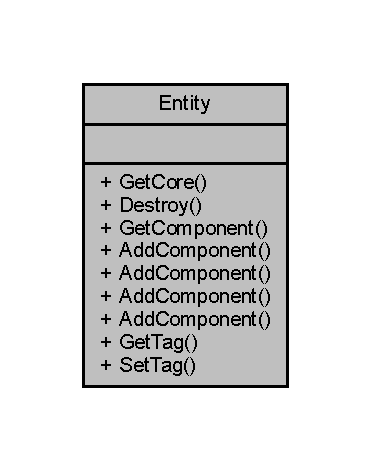
\includegraphics[width=178pt]{class_entity__coll__graph}
\end{center}
\end{figure}
\subsection*{Public Member Functions}
\begin{DoxyCompactItemize}
\item 
std\+::shared\+\_\+ptr$<$ \mbox{\hyperlink{class_core}{Core}} $>$ \mbox{\hyperlink{class_entity_aca8a5ff6e980db6f834d841a73dfbf89}{Get\+Core}} ()
\item 
void \mbox{\hyperlink{class_entity_aa75151fc607686b42d27f8c3ba73143d}{Destroy}} ()
\item 
{\footnotesize template$<$typename T $>$ }\\std\+::shared\+\_\+ptr$<$ T $>$ \mbox{\hyperlink{class_entity_ad5cf8774322cc838147e43866a475546}{Get\+Component}} ()
\item 
{\footnotesize template$<$typename T $>$ }\\std\+::shared\+\_\+ptr$<$ T $>$ \mbox{\hyperlink{class_entity_ad81bdf8285a9da23658d48dd5aaebb03}{Add\+Component}} ()
\item 
{\footnotesize template$<$typename T , typename A $>$ }\\std\+::shared\+\_\+ptr$<$ T $>$ \mbox{\hyperlink{class_entity_a9479c2ee06931b01c9b9012191de8dc7}{Add\+Component}} (A a)
\item 
{\footnotesize template$<$typename T , typename A , typename B $>$ }\\std\+::shared\+\_\+ptr$<$ T $>$ \mbox{\hyperlink{class_entity_aa07de6a1691dc07198feb401e273139e}{Add\+Component}} (A a, B b)
\item 
{\footnotesize template$<$typename T , typename A , typename B , typename C $>$ }\\std\+::shared\+\_\+ptr$<$ T $>$ \mbox{\hyperlink{class_entity_abe12552792daa14156ade47eb8db1933}{Add\+Component}} (A a, B b, C c)
\item 
std\+::string \mbox{\hyperlink{class_entity_a75b54507da9a1178db1f742cc49fcba1}{Get\+Tag}} ()
\item 
void \mbox{\hyperlink{class_entity_ac5da9f659ddd64da2c4c18ee6346d320}{Set\+Tag}} (std\+::string \+\_\+tag)
\end{DoxyCompactItemize}
\subsection*{Friends}
\begin{DoxyCompactItemize}
\item 
class \mbox{\hyperlink{class_entity_a4107254ac74f90d4f91e810d755b98c2}{Core}}
\end{DoxyCompactItemize}


\subsection{Member Function Documentation}
\mbox{\Hypertarget{class_entity_ad81bdf8285a9da23658d48dd5aaebb03}\label{class_entity_ad81bdf8285a9da23658d48dd5aaebb03}} 
\index{Entity@{Entity}!Add\+Component@{Add\+Component}}
\index{Add\+Component@{Add\+Component}!Entity@{Entity}}
\subsubsection{\texorpdfstring{Add\+Component()}{AddComponent()}\hspace{0.1cm}{\footnotesize\ttfamily [1/4]}}
{\footnotesize\ttfamily template$<$typename T $>$ \\
std\+::shared\+\_\+ptr$<$T$>$ Entity\+::\+Add\+Component (\begin{DoxyParamCaption}{ }\end{DoxyParamCaption})\hspace{0.3cm}{\ttfamily [inline]}}

\mbox{\Hypertarget{class_entity_a9479c2ee06931b01c9b9012191de8dc7}\label{class_entity_a9479c2ee06931b01c9b9012191de8dc7}} 
\index{Entity@{Entity}!Add\+Component@{Add\+Component}}
\index{Add\+Component@{Add\+Component}!Entity@{Entity}}
\subsubsection{\texorpdfstring{Add\+Component()}{AddComponent()}\hspace{0.1cm}{\footnotesize\ttfamily [2/4]}}
{\footnotesize\ttfamily template$<$typename T , typename A $>$ \\
std\+::shared\+\_\+ptr$<$T$>$ Entity\+::\+Add\+Component (\begin{DoxyParamCaption}\item[{A}]{a }\end{DoxyParamCaption})\hspace{0.3cm}{\ttfamily [inline]}}

\mbox{\Hypertarget{class_entity_aa07de6a1691dc07198feb401e273139e}\label{class_entity_aa07de6a1691dc07198feb401e273139e}} 
\index{Entity@{Entity}!Add\+Component@{Add\+Component}}
\index{Add\+Component@{Add\+Component}!Entity@{Entity}}
\subsubsection{\texorpdfstring{Add\+Component()}{AddComponent()}\hspace{0.1cm}{\footnotesize\ttfamily [3/4]}}
{\footnotesize\ttfamily template$<$typename T , typename A , typename B $>$ \\
std\+::shared\+\_\+ptr$<$T$>$ Entity\+::\+Add\+Component (\begin{DoxyParamCaption}\item[{A}]{a,  }\item[{B}]{b }\end{DoxyParamCaption})\hspace{0.3cm}{\ttfamily [inline]}}

\mbox{\Hypertarget{class_entity_abe12552792daa14156ade47eb8db1933}\label{class_entity_abe12552792daa14156ade47eb8db1933}} 
\index{Entity@{Entity}!Add\+Component@{Add\+Component}}
\index{Add\+Component@{Add\+Component}!Entity@{Entity}}
\subsubsection{\texorpdfstring{Add\+Component()}{AddComponent()}\hspace{0.1cm}{\footnotesize\ttfamily [4/4]}}
{\footnotesize\ttfamily template$<$typename T , typename A , typename B , typename C $>$ \\
std\+::shared\+\_\+ptr$<$T$>$ Entity\+::\+Add\+Component (\begin{DoxyParamCaption}\item[{A}]{a,  }\item[{B}]{b,  }\item[{C}]{c }\end{DoxyParamCaption})\hspace{0.3cm}{\ttfamily [inline]}}

\mbox{\Hypertarget{class_entity_aa75151fc607686b42d27f8c3ba73143d}\label{class_entity_aa75151fc607686b42d27f8c3ba73143d}} 
\index{Entity@{Entity}!Destroy@{Destroy}}
\index{Destroy@{Destroy}!Entity@{Entity}}
\subsubsection{\texorpdfstring{Destroy()}{Destroy()}}
{\footnotesize\ttfamily void Entity\+::\+Destroy (\begin{DoxyParamCaption}{ }\end{DoxyParamCaption})}

\mbox{\Hypertarget{class_entity_ad5cf8774322cc838147e43866a475546}\label{class_entity_ad5cf8774322cc838147e43866a475546}} 
\index{Entity@{Entity}!Get\+Component@{Get\+Component}}
\index{Get\+Component@{Get\+Component}!Entity@{Entity}}
\subsubsection{\texorpdfstring{Get\+Component()}{GetComponent()}}
{\footnotesize\ttfamily template$<$typename T $>$ \\
std\+::shared\+\_\+ptr$<$T$>$ Entity\+::\+Get\+Component (\begin{DoxyParamCaption}{ }\end{DoxyParamCaption})\hspace{0.3cm}{\ttfamily [inline]}}

\mbox{\Hypertarget{class_entity_aca8a5ff6e980db6f834d841a73dfbf89}\label{class_entity_aca8a5ff6e980db6f834d841a73dfbf89}} 
\index{Entity@{Entity}!Get\+Core@{Get\+Core}}
\index{Get\+Core@{Get\+Core}!Entity@{Entity}}
\subsubsection{\texorpdfstring{Get\+Core()}{GetCore()}}
{\footnotesize\ttfamily std\+::shared\+\_\+ptr$<$ \mbox{\hyperlink{class_core}{Core}} $>$ Entity\+::\+Get\+Core (\begin{DoxyParamCaption}{ }\end{DoxyParamCaption})}

\mbox{\Hypertarget{class_entity_a75b54507da9a1178db1f742cc49fcba1}\label{class_entity_a75b54507da9a1178db1f742cc49fcba1}} 
\index{Entity@{Entity}!Get\+Tag@{Get\+Tag}}
\index{Get\+Tag@{Get\+Tag}!Entity@{Entity}}
\subsubsection{\texorpdfstring{Get\+Tag()}{GetTag()}}
{\footnotesize\ttfamily std\+::string Entity\+::\+Get\+Tag (\begin{DoxyParamCaption}{ }\end{DoxyParamCaption})\hspace{0.3cm}{\ttfamily [inline]}}

\mbox{\Hypertarget{class_entity_ac5da9f659ddd64da2c4c18ee6346d320}\label{class_entity_ac5da9f659ddd64da2c4c18ee6346d320}} 
\index{Entity@{Entity}!Set\+Tag@{Set\+Tag}}
\index{Set\+Tag@{Set\+Tag}!Entity@{Entity}}
\subsubsection{\texorpdfstring{Set\+Tag()}{SetTag()}}
{\footnotesize\ttfamily void Entity\+::\+Set\+Tag (\begin{DoxyParamCaption}\item[{std\+::string}]{\+\_\+tag }\end{DoxyParamCaption})\hspace{0.3cm}{\ttfamily [inline]}}



\subsection{Friends And Related Function Documentation}
\mbox{\Hypertarget{class_entity_a4107254ac74f90d4f91e810d755b98c2}\label{class_entity_a4107254ac74f90d4f91e810d755b98c2}} 
\index{Entity@{Entity}!Core@{Core}}
\index{Core@{Core}!Entity@{Entity}}
\subsubsection{\texorpdfstring{Core}{Core}}
{\footnotesize\ttfamily friend class \mbox{\hyperlink{class_core}{Core}}\hspace{0.3cm}{\ttfamily [friend]}}



The documentation for this class was generated from the following files\+:\begin{DoxyCompactItemize}
\item 
\mbox{\hyperlink{_entity_8h}{Entity.\+h}}\item 
\mbox{\hyperlink{_entity_8cpp}{Entity.\+cpp}}\end{DoxyCompactItemize}

\hypertarget{class_environment}{}\section{Environment Class Reference}
\label{class_environment}\index{Environment@{Environment}}


{\ttfamily \#include $<$Environment.\+h$>$}



Collaboration diagram for Environment\+:
\nopagebreak
\begin{figure}[H]
\begin{center}
\leavevmode
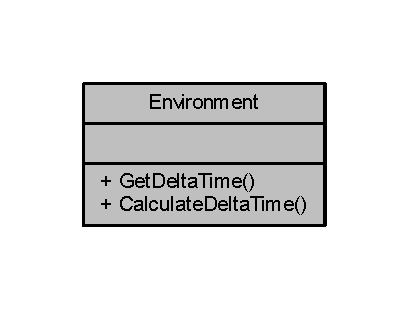
\includegraphics[width=196pt]{class_environment__coll__graph}
\end{center}
\end{figure}
\subsection*{Public Member Functions}
\begin{DoxyCompactItemize}
\item 
float \mbox{\hyperlink{class_environment_a4444c726d8d25a102ad12721385e3c3b}{Get\+Delta\+Time}} ()
\item 
void \mbox{\hyperlink{class_environment_a1820a270c6d400963e8c26efe075c26d}{Calculate\+Delta\+Time}} ()
\end{DoxyCompactItemize}


\subsection{Member Function Documentation}
\mbox{\Hypertarget{class_environment_a1820a270c6d400963e8c26efe075c26d}\label{class_environment_a1820a270c6d400963e8c26efe075c26d}} 
\index{Environment@{Environment}!Calculate\+Delta\+Time@{Calculate\+Delta\+Time}}
\index{Calculate\+Delta\+Time@{Calculate\+Delta\+Time}!Environment@{Environment}}
\subsubsection{\texorpdfstring{Calculate\+Delta\+Time()}{CalculateDeltaTime()}}
{\footnotesize\ttfamily void Environment\+::\+Calculate\+Delta\+Time (\begin{DoxyParamCaption}{ }\end{DoxyParamCaption})}

\mbox{\Hypertarget{class_environment_a4444c726d8d25a102ad12721385e3c3b}\label{class_environment_a4444c726d8d25a102ad12721385e3c3b}} 
\index{Environment@{Environment}!Get\+Delta\+Time@{Get\+Delta\+Time}}
\index{Get\+Delta\+Time@{Get\+Delta\+Time}!Environment@{Environment}}
\subsubsection{\texorpdfstring{Get\+Delta\+Time()}{GetDeltaTime()}}
{\footnotesize\ttfamily float Environment\+::\+Get\+Delta\+Time (\begin{DoxyParamCaption}{ }\end{DoxyParamCaption})\hspace{0.3cm}{\ttfamily [inline]}}



The documentation for this class was generated from the following files\+:\begin{DoxyCompactItemize}
\item 
\mbox{\hyperlink{_environment_8h}{Environment.\+h}}\item 
\mbox{\hyperlink{_environment_8cpp}{Environment.\+cpp}}\end{DoxyCompactItemize}

\hypertarget{class_exception}{}\section{Exception Class Reference}
\label{class_exception}\index{Exception@{Exception}}


{\ttfamily \#include $<$Exception.\+h$>$}



Inheritance diagram for Exception\+:
\nopagebreak
\begin{figure}[H]
\begin{center}
\leavevmode
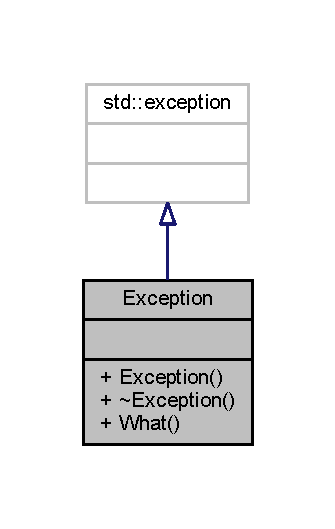
\includegraphics[width=161pt]{class_exception__inherit__graph}
\end{center}
\end{figure}


Collaboration diagram for Exception\+:
\nopagebreak
\begin{figure}[H]
\begin{center}
\leavevmode
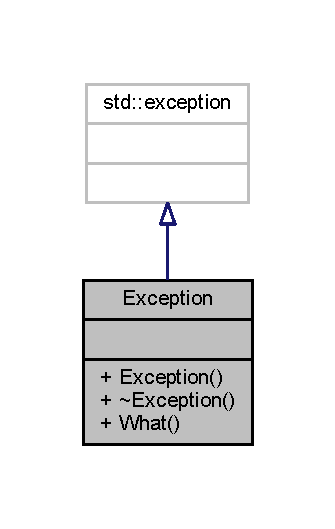
\includegraphics[width=161pt]{class_exception__coll__graph}
\end{center}
\end{figure}
\subsection*{Public Member Functions}
\begin{DoxyCompactItemize}
\item 
\mbox{\hyperlink{class_exception_ad17bdcd9d14fcb0fa63a2a78c8e8ce7f}{Exception}} (std\+::string \+\_\+message)
\item 
\mbox{\hyperlink{class_exception_a6b214cd8627d0968bdeebc1fbb9556b8}{$\sim$\+Exception}} ()  throw ()
\item 
const char $\ast$ \mbox{\hyperlink{class_exception_a074e6e0496fe2cd72a8677615e7d1f61}{What}} ()
\end{DoxyCompactItemize}


\subsection{Constructor \& Destructor Documentation}
\mbox{\Hypertarget{class_exception_ad17bdcd9d14fcb0fa63a2a78c8e8ce7f}\label{class_exception_ad17bdcd9d14fcb0fa63a2a78c8e8ce7f}} 
\index{Exception@{Exception}!Exception@{Exception}}
\index{Exception@{Exception}!Exception@{Exception}}
\subsubsection{\texorpdfstring{Exception()}{Exception()}}
{\footnotesize\ttfamily Exception\+::\+Exception (\begin{DoxyParamCaption}\item[{std\+::string}]{\+\_\+message }\end{DoxyParamCaption})}

\mbox{\Hypertarget{class_exception_a6b214cd8627d0968bdeebc1fbb9556b8}\label{class_exception_a6b214cd8627d0968bdeebc1fbb9556b8}} 
\index{Exception@{Exception}!````~Exception@{$\sim$\+Exception}}
\index{````~Exception@{$\sim$\+Exception}!Exception@{Exception}}
\subsubsection{\texorpdfstring{$\sim$\+Exception()}{~Exception()}}
{\footnotesize\ttfamily Exception\+::$\sim$\+Exception (\begin{DoxyParamCaption}{ }\end{DoxyParamCaption}) throw  ) }



\subsection{Member Function Documentation}
\mbox{\Hypertarget{class_exception_a074e6e0496fe2cd72a8677615e7d1f61}\label{class_exception_a074e6e0496fe2cd72a8677615e7d1f61}} 
\index{Exception@{Exception}!What@{What}}
\index{What@{What}!Exception@{Exception}}
\subsubsection{\texorpdfstring{What()}{What()}}
{\footnotesize\ttfamily const char$\ast$ Exception\+::\+What (\begin{DoxyParamCaption}{ }\end{DoxyParamCaption})}



The documentation for this class was generated from the following file\+:\begin{DoxyCompactItemize}
\item 
\mbox{\hyperlink{_exception_8h}{Exception.\+h}}\end{DoxyCompactItemize}

\hypertarget{class_game_object}{}\section{Game\+Object Class Reference}
\label{class_game_object}\index{Game\+Object@{Game\+Object}}


{\ttfamily \#include $<$Game\+Engine.\+h$>$}



Collaboration diagram for Game\+Object\+:
\nopagebreak
\begin{figure}[H]
\begin{center}
\leavevmode
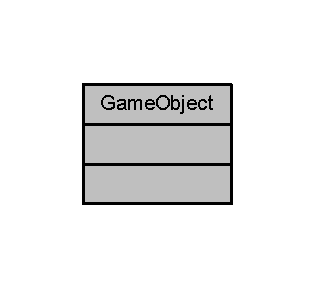
\includegraphics[width=151pt]{class_game_object__coll__graph}
\end{center}
\end{figure}


The documentation for this class was generated from the following file\+:\begin{DoxyCompactItemize}
\item 
\mbox{\hyperlink{_game_engine_8h}{Game\+Engine.\+h}}\end{DoxyCompactItemize}

\hypertarget{class_keyboard_handler}{}\section{Keyboard\+Handler Class Reference}
\label{class_keyboard_handler}\index{Keyboard\+Handler@{Keyboard\+Handler}}


{\ttfamily \#include $<$Keyboard\+Handler.\+h$>$}



Collaboration diagram for Keyboard\+Handler\+:
\nopagebreak
\begin{figure}[H]
\begin{center}
\leavevmode
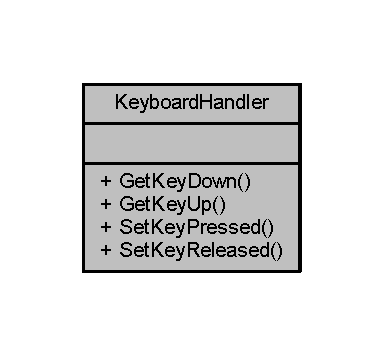
\includegraphics[width=184pt]{class_keyboard_handler__coll__graph}
\end{center}
\end{figure}
\subsection*{Public Member Functions}
\begin{DoxyCompactItemize}
\item 
bool \mbox{\hyperlink{class_keyboard_handler_accf4e35731010260a4f519c929d00a64}{Get\+Key\+Down}} (std\+::string \+\_\+key)
\item 
bool \mbox{\hyperlink{class_keyboard_handler_ad184d06a6bf5d2d1db362e79a8073d98}{Get\+Key\+Up}} (std\+::string \+\_\+key)
\item 
void \mbox{\hyperlink{class_keyboard_handler_a166c8d62ec7c01cb155e7ba47007501a}{Set\+Key\+Pressed}} (S\+D\+L\+\_\+\+Keycode \+\_\+key)
\item 
void \mbox{\hyperlink{class_keyboard_handler_a696a4ddd0a75c79f220c424bd4bd1889}{Set\+Key\+Released}} (S\+D\+L\+\_\+\+Keycode \+\_\+key)
\end{DoxyCompactItemize}


\subsection{Member Function Documentation}
\mbox{\Hypertarget{class_keyboard_handler_accf4e35731010260a4f519c929d00a64}\label{class_keyboard_handler_accf4e35731010260a4f519c929d00a64}} 
\index{Keyboard\+Handler@{Keyboard\+Handler}!Get\+Key\+Down@{Get\+Key\+Down}}
\index{Get\+Key\+Down@{Get\+Key\+Down}!Keyboard\+Handler@{Keyboard\+Handler}}
\subsubsection{\texorpdfstring{Get\+Key\+Down()}{GetKeyDown()}}
{\footnotesize\ttfamily bool Keyboard\+Handler\+::\+Get\+Key\+Down (\begin{DoxyParamCaption}\item[{std\+::string}]{\+\_\+key }\end{DoxyParamCaption})}

\mbox{\Hypertarget{class_keyboard_handler_ad184d06a6bf5d2d1db362e79a8073d98}\label{class_keyboard_handler_ad184d06a6bf5d2d1db362e79a8073d98}} 
\index{Keyboard\+Handler@{Keyboard\+Handler}!Get\+Key\+Up@{Get\+Key\+Up}}
\index{Get\+Key\+Up@{Get\+Key\+Up}!Keyboard\+Handler@{Keyboard\+Handler}}
\subsubsection{\texorpdfstring{Get\+Key\+Up()}{GetKeyUp()}}
{\footnotesize\ttfamily bool Keyboard\+Handler\+::\+Get\+Key\+Up (\begin{DoxyParamCaption}\item[{std\+::string}]{\+\_\+key }\end{DoxyParamCaption})}

\mbox{\Hypertarget{class_keyboard_handler_a166c8d62ec7c01cb155e7ba47007501a}\label{class_keyboard_handler_a166c8d62ec7c01cb155e7ba47007501a}} 
\index{Keyboard\+Handler@{Keyboard\+Handler}!Set\+Key\+Pressed@{Set\+Key\+Pressed}}
\index{Set\+Key\+Pressed@{Set\+Key\+Pressed}!Keyboard\+Handler@{Keyboard\+Handler}}
\subsubsection{\texorpdfstring{Set\+Key\+Pressed()}{SetKeyPressed()}}
{\footnotesize\ttfamily void Keyboard\+Handler\+::\+Set\+Key\+Pressed (\begin{DoxyParamCaption}\item[{S\+D\+L\+\_\+\+Keycode}]{\+\_\+key }\end{DoxyParamCaption})}

\mbox{\Hypertarget{class_keyboard_handler_a696a4ddd0a75c79f220c424bd4bd1889}\label{class_keyboard_handler_a696a4ddd0a75c79f220c424bd4bd1889}} 
\index{Keyboard\+Handler@{Keyboard\+Handler}!Set\+Key\+Released@{Set\+Key\+Released}}
\index{Set\+Key\+Released@{Set\+Key\+Released}!Keyboard\+Handler@{Keyboard\+Handler}}
\subsubsection{\texorpdfstring{Set\+Key\+Released()}{SetKeyReleased()}}
{\footnotesize\ttfamily void Keyboard\+Handler\+::\+Set\+Key\+Released (\begin{DoxyParamCaption}\item[{S\+D\+L\+\_\+\+Keycode}]{\+\_\+key }\end{DoxyParamCaption})}



The documentation for this class was generated from the following files\+:\begin{DoxyCompactItemize}
\item 
\mbox{\hyperlink{_keyboard_handler_8h}{Keyboard\+Handler.\+h}}\item 
\mbox{\hyperlink{_keyboard_handler_8cpp}{Keyboard\+Handler.\+cpp}}\end{DoxyCompactItemize}

\hypertarget{class_material}{}\section{Material Class Reference}
\label{class_material}\index{Material@{Material}}


{\ttfamily \#include $<$Material.\+h$>$}



Inheritance diagram for Material\+:
\nopagebreak
\begin{figure}[H]
\begin{center}
\leavevmode
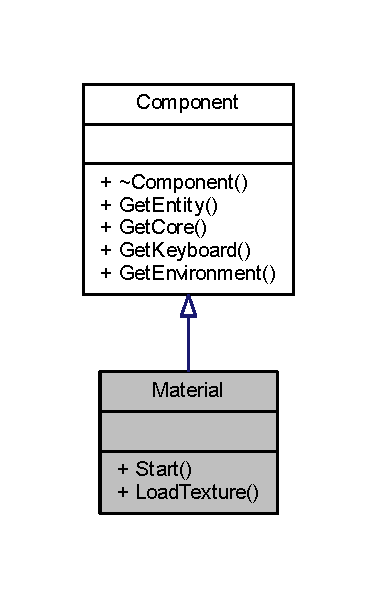
\includegraphics[width=181pt]{class_material__inherit__graph}
\end{center}
\end{figure}


Collaboration diagram for Material\+:
\nopagebreak
\begin{figure}[H]
\begin{center}
\leavevmode
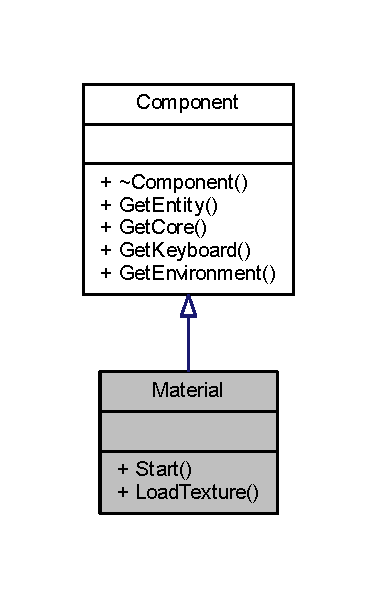
\includegraphics[width=181pt]{class_material__coll__graph}
\end{center}
\end{figure}
\subsection*{Public Member Functions}
\begin{DoxyCompactItemize}
\item 
void \mbox{\hyperlink{class_material_a8fcc1a8e83981ddd45c746c7ca98e46c}{Start}} (std\+::string \+\_\+image\+Path)
\item 
void \mbox{\hyperlink{class_material_ae9aac906f4d3d12b8c97908647405111}{Load\+Texture}} (std\+::string \+\_\+image\+Path)
\end{DoxyCompactItemize}


\subsection{Member Function Documentation}
\mbox{\Hypertarget{class_material_ae9aac906f4d3d12b8c97908647405111}\label{class_material_ae9aac906f4d3d12b8c97908647405111}} 
\index{Material@{Material}!Load\+Texture@{Load\+Texture}}
\index{Load\+Texture@{Load\+Texture}!Material@{Material}}
\subsubsection{\texorpdfstring{Load\+Texture()}{LoadTexture()}}
{\footnotesize\ttfamily void Material\+::\+Load\+Texture (\begin{DoxyParamCaption}\item[{std\+::string}]{\+\_\+image\+Path }\end{DoxyParamCaption})}

Here is the call graph for this function\+:
\nopagebreak
\begin{figure}[H]
\begin{center}
\leavevmode
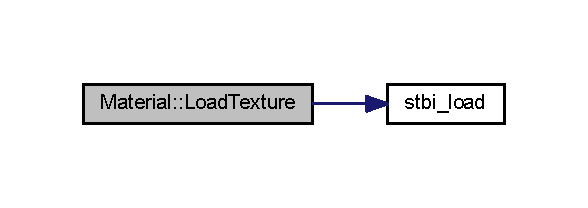
\includegraphics[width=282pt]{class_material_ae9aac906f4d3d12b8c97908647405111_cgraph}
\end{center}
\end{figure}
Here is the caller graph for this function\+:
\nopagebreak
\begin{figure}[H]
\begin{center}
\leavevmode
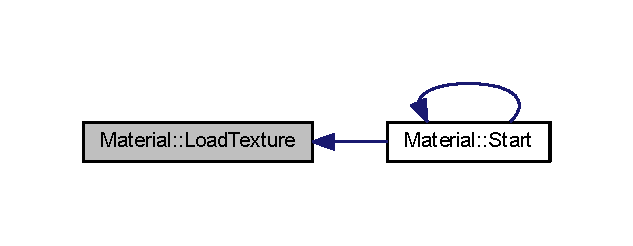
\includegraphics[width=304pt]{class_material_ae9aac906f4d3d12b8c97908647405111_icgraph}
\end{center}
\end{figure}
\mbox{\Hypertarget{class_material_a8fcc1a8e83981ddd45c746c7ca98e46c}\label{class_material_a8fcc1a8e83981ddd45c746c7ca98e46c}} 
\index{Material@{Material}!Start@{Start}}
\index{Start@{Start}!Material@{Material}}
\subsubsection{\texorpdfstring{Start()}{Start()}}
{\footnotesize\ttfamily void Material\+::\+Start (\begin{DoxyParamCaption}\item[{std\+::string}]{\+\_\+image\+Path }\end{DoxyParamCaption})}

Here is the call graph for this function\+:
\nopagebreak
\begin{figure}[H]
\begin{center}
\leavevmode
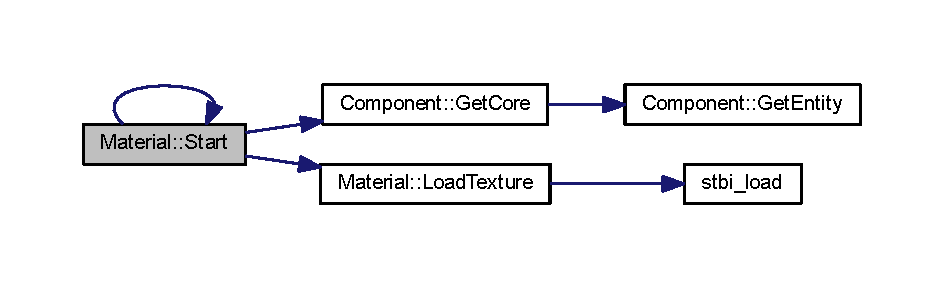
\includegraphics[width=350pt]{class_material_a8fcc1a8e83981ddd45c746c7ca98e46c_cgraph}
\end{center}
\end{figure}
Here is the caller graph for this function\+:
\nopagebreak
\begin{figure}[H]
\begin{center}
\leavevmode
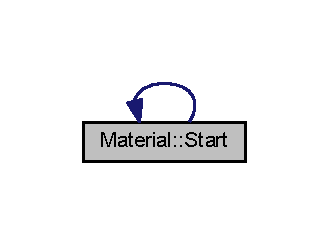
\includegraphics[width=158pt]{class_material_a8fcc1a8e83981ddd45c746c7ca98e46c_icgraph}
\end{center}
\end{figure}


The documentation for this class was generated from the following files\+:\begin{DoxyCompactItemize}
\item 
\mbox{\hyperlink{_material_8h}{Material.\+h}}\item 
\mbox{\hyperlink{_material_8cpp}{Material.\+cpp}}\end{DoxyCompactItemize}

\hypertarget{struct_mat_resource}{}\section{Mat\+Resource Struct Reference}
\label{struct_mat_resource}\index{Mat\+Resource@{Mat\+Resource}}


{\ttfamily \#include $<$Resources.\+h$>$}



Collaboration diagram for Mat\+Resource\+:
\nopagebreak
\begin{figure}[H]
\begin{center}
\leavevmode
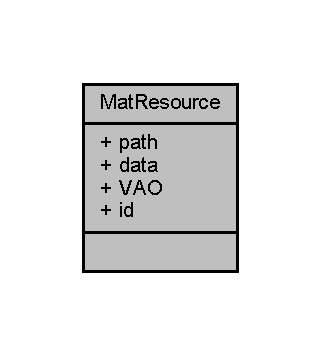
\includegraphics[width=154pt]{struct_mat_resource__coll__graph}
\end{center}
\end{figure}
\subsection*{Public Attributes}
\begin{DoxyCompactItemize}
\item 
std\+::string \mbox{\hyperlink{struct_mat_resource_ad4586d33efdbb0a46137f01eb22043f8}{path}}
\item 
unsigned char $\ast$ \mbox{\hyperlink{struct_mat_resource_ae258c8d165fa65017eb07be4787bb0ff}{data}}
\item 
std\+::shared\+\_\+ptr$<$ \mbox{\hyperlink{class_vertex_array}{Vertex\+Array}} $>$ \mbox{\hyperlink{struct_mat_resource_ab208f0b2bcb3478c64ee208ebceb1f18}{V\+AO}}
\item 
G\+Luint \mbox{\hyperlink{struct_mat_resource_ab05a8aa12860a2f550a9c4ff0fb1ce4e}{id}}
\end{DoxyCompactItemize}


\subsection{Member Data Documentation}
\mbox{\Hypertarget{struct_mat_resource_ae258c8d165fa65017eb07be4787bb0ff}\label{struct_mat_resource_ae258c8d165fa65017eb07be4787bb0ff}} 
\index{Mat\+Resource@{Mat\+Resource}!data@{data}}
\index{data@{data}!Mat\+Resource@{Mat\+Resource}}
\subsubsection{\texorpdfstring{data}{data}}
{\footnotesize\ttfamily unsigned char$\ast$ Mat\+Resource\+::data}

\mbox{\Hypertarget{struct_mat_resource_ab05a8aa12860a2f550a9c4ff0fb1ce4e}\label{struct_mat_resource_ab05a8aa12860a2f550a9c4ff0fb1ce4e}} 
\index{Mat\+Resource@{Mat\+Resource}!id@{id}}
\index{id@{id}!Mat\+Resource@{Mat\+Resource}}
\subsubsection{\texorpdfstring{id}{id}}
{\footnotesize\ttfamily G\+Luint Mat\+Resource\+::id}

\mbox{\Hypertarget{struct_mat_resource_ad4586d33efdbb0a46137f01eb22043f8}\label{struct_mat_resource_ad4586d33efdbb0a46137f01eb22043f8}} 
\index{Mat\+Resource@{Mat\+Resource}!path@{path}}
\index{path@{path}!Mat\+Resource@{Mat\+Resource}}
\subsubsection{\texorpdfstring{path}{path}}
{\footnotesize\ttfamily std\+::string Mat\+Resource\+::path}

\mbox{\Hypertarget{struct_mat_resource_ab208f0b2bcb3478c64ee208ebceb1f18}\label{struct_mat_resource_ab208f0b2bcb3478c64ee208ebceb1f18}} 
\index{Mat\+Resource@{Mat\+Resource}!V\+AO@{V\+AO}}
\index{V\+AO@{V\+AO}!Mat\+Resource@{Mat\+Resource}}
\subsubsection{\texorpdfstring{V\+AO}{VAO}}
{\footnotesize\ttfamily std\+::shared\+\_\+ptr$<$\mbox{\hyperlink{class_vertex_array}{Vertex\+Array}}$>$ Mat\+Resource\+::\+V\+AO}



The documentation for this struct was generated from the following file\+:\begin{DoxyCompactItemize}
\item 
\mbox{\hyperlink{_resources_8h}{Resources.\+h}}\end{DoxyCompactItemize}

\hypertarget{class_mesh_renderer}{}\section{Mesh\+Renderer Class Reference}
\label{class_mesh_renderer}\index{Mesh\+Renderer@{Mesh\+Renderer}}


{\ttfamily \#include $<$Mesh\+Renderer.\+h$>$}



Inheritance diagram for Mesh\+Renderer\+:
\nopagebreak
\begin{figure}[H]
\begin{center}
\leavevmode
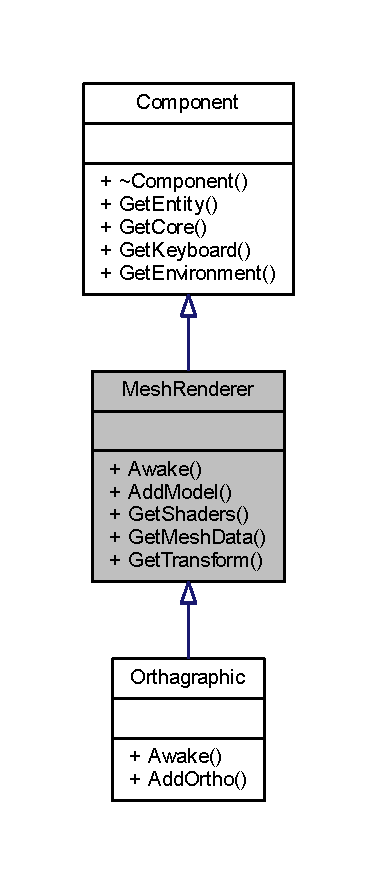
\includegraphics[width=181pt]{class_mesh_renderer__inherit__graph}
\end{center}
\end{figure}


Collaboration diagram for Mesh\+Renderer\+:
\nopagebreak
\begin{figure}[H]
\begin{center}
\leavevmode
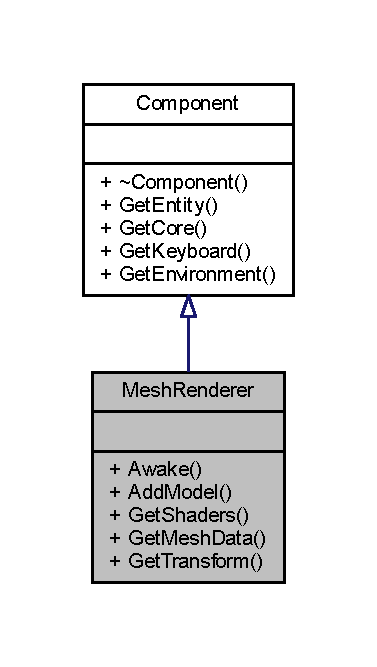
\includegraphics[width=181pt]{class_mesh_renderer__coll__graph}
\end{center}
\end{figure}
\subsection*{Public Member Functions}
\begin{DoxyCompactItemize}
\item 
void \mbox{\hyperlink{class_mesh_renderer_a3fc0e9658d3b9a53e3559cb9b939aeb9}{Awake}} ()
\item 
void \mbox{\hyperlink{class_mesh_renderer_a90798e723067ca8c721f0c96c1609972}{Add\+Model}} (std\+::string \+\_\+model\+Path, std\+::string \+\_\+vertex\+Path, std\+::string \+\_\+frag\+Path)
\item 
std\+::shared\+\_\+ptr$<$ \mbox{\hyperlink{class_shader_program}{Shader\+Program}} $>$ \mbox{\hyperlink{class_mesh_renderer_a07be90e4601d54e0870854cc91dc018c}{Get\+Shaders}} ()
\item 
std\+::shared\+\_\+ptr$<$ \mbox{\hyperlink{class_vertex_array}{Vertex\+Array}} $>$ \mbox{\hyperlink{class_mesh_renderer_a2924155f99c9276a2089ff618f9016c8}{Get\+Mesh\+Data}} ()
\item 
std\+::shared\+\_\+ptr$<$ \mbox{\hyperlink{class_transform}{Transform}} $>$ \mbox{\hyperlink{class_mesh_renderer_a89beac4cf0a91a275686c5f5507af465}{Get\+Transform}} ()
\end{DoxyCompactItemize}


\subsection{Member Function Documentation}
\mbox{\Hypertarget{class_mesh_renderer_a90798e723067ca8c721f0c96c1609972}\label{class_mesh_renderer_a90798e723067ca8c721f0c96c1609972}} 
\index{Mesh\+Renderer@{Mesh\+Renderer}!Add\+Model@{Add\+Model}}
\index{Add\+Model@{Add\+Model}!Mesh\+Renderer@{Mesh\+Renderer}}
\subsubsection{\texorpdfstring{Add\+Model()}{AddModel()}}
{\footnotesize\ttfamily void Mesh\+Renderer\+::\+Add\+Model (\begin{DoxyParamCaption}\item[{std\+::string}]{\+\_\+model\+Path,  }\item[{std\+::string}]{\+\_\+vertex\+Path,  }\item[{std\+::string}]{\+\_\+frag\+Path }\end{DoxyParamCaption})}

Here is the call graph for this function\+:
\nopagebreak
\begin{figure}[H]
\begin{center}
\leavevmode
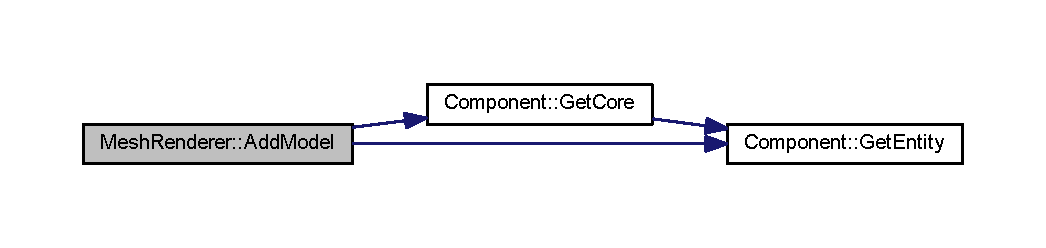
\includegraphics[width=350pt]{class_mesh_renderer_a90798e723067ca8c721f0c96c1609972_cgraph}
\end{center}
\end{figure}
Here is the caller graph for this function\+:
\nopagebreak
\begin{figure}[H]
\begin{center}
\leavevmode
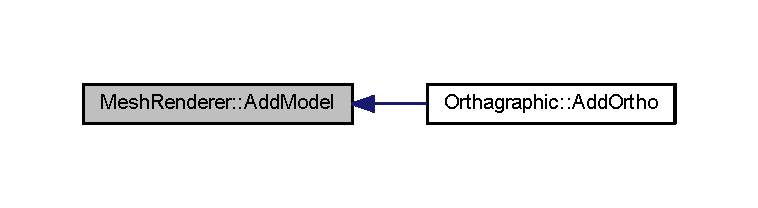
\includegraphics[width=350pt]{class_mesh_renderer_a90798e723067ca8c721f0c96c1609972_icgraph}
\end{center}
\end{figure}
\mbox{\Hypertarget{class_mesh_renderer_a3fc0e9658d3b9a53e3559cb9b939aeb9}\label{class_mesh_renderer_a3fc0e9658d3b9a53e3559cb9b939aeb9}} 
\index{Mesh\+Renderer@{Mesh\+Renderer}!Awake@{Awake}}
\index{Awake@{Awake}!Mesh\+Renderer@{Mesh\+Renderer}}
\subsubsection{\texorpdfstring{Awake()}{Awake()}}
{\footnotesize\ttfamily void Mesh\+Renderer\+::\+Awake (\begin{DoxyParamCaption}{ }\end{DoxyParamCaption})\hspace{0.3cm}{\ttfamily [virtual]}}



Reimplemented from \mbox{\hyperlink{class_component}{Component}}.



Reimplemented in \mbox{\hyperlink{class_orthagraphic_a62f9d1b5d54623252bc3d15eba1e7181}{Orthagraphic}}.

\mbox{\Hypertarget{class_mesh_renderer_a2924155f99c9276a2089ff618f9016c8}\label{class_mesh_renderer_a2924155f99c9276a2089ff618f9016c8}} 
\index{Mesh\+Renderer@{Mesh\+Renderer}!Get\+Mesh\+Data@{Get\+Mesh\+Data}}
\index{Get\+Mesh\+Data@{Get\+Mesh\+Data}!Mesh\+Renderer@{Mesh\+Renderer}}
\subsubsection{\texorpdfstring{Get\+Mesh\+Data()}{GetMeshData()}}
{\footnotesize\ttfamily std\+::shared\+\_\+ptr$<$\mbox{\hyperlink{class_vertex_array}{Vertex\+Array}}$>$ Mesh\+Renderer\+::\+Get\+Mesh\+Data (\begin{DoxyParamCaption}{ }\end{DoxyParamCaption})\hspace{0.3cm}{\ttfamily [inline]}}

\mbox{\Hypertarget{class_mesh_renderer_a07be90e4601d54e0870854cc91dc018c}\label{class_mesh_renderer_a07be90e4601d54e0870854cc91dc018c}} 
\index{Mesh\+Renderer@{Mesh\+Renderer}!Get\+Shaders@{Get\+Shaders}}
\index{Get\+Shaders@{Get\+Shaders}!Mesh\+Renderer@{Mesh\+Renderer}}
\subsubsection{\texorpdfstring{Get\+Shaders()}{GetShaders()}}
{\footnotesize\ttfamily std\+::shared\+\_\+ptr$<$\mbox{\hyperlink{class_shader_program}{Shader\+Program}}$>$ Mesh\+Renderer\+::\+Get\+Shaders (\begin{DoxyParamCaption}{ }\end{DoxyParamCaption})\hspace{0.3cm}{\ttfamily [inline]}}

Here is the caller graph for this function\+:
\nopagebreak
\begin{figure}[H]
\begin{center}
\leavevmode
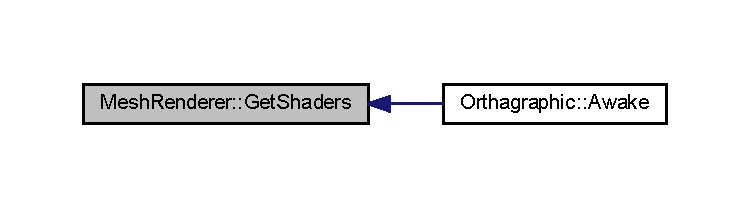
\includegraphics[width=350pt]{class_mesh_renderer_a07be90e4601d54e0870854cc91dc018c_icgraph}
\end{center}
\end{figure}
\mbox{\Hypertarget{class_mesh_renderer_a89beac4cf0a91a275686c5f5507af465}\label{class_mesh_renderer_a89beac4cf0a91a275686c5f5507af465}} 
\index{Mesh\+Renderer@{Mesh\+Renderer}!Get\+Transform@{Get\+Transform}}
\index{Get\+Transform@{Get\+Transform}!Mesh\+Renderer@{Mesh\+Renderer}}
\subsubsection{\texorpdfstring{Get\+Transform()}{GetTransform()}}
{\footnotesize\ttfamily std\+::shared\+\_\+ptr$<$\mbox{\hyperlink{class_transform}{Transform}}$>$ Mesh\+Renderer\+::\+Get\+Transform (\begin{DoxyParamCaption}{ }\end{DoxyParamCaption})\hspace{0.3cm}{\ttfamily [inline]}}



The documentation for this class was generated from the following files\+:\begin{DoxyCompactItemize}
\item 
\mbox{\hyperlink{_mesh_renderer_8h}{Mesh\+Renderer.\+h}}\item 
\mbox{\hyperlink{_mesh_renderer_8cpp}{Mesh\+Renderer.\+cpp}}\end{DoxyCompactItemize}

\hypertarget{struct_mesh_resource}{}\section{Mesh\+Resource Struct Reference}
\label{struct_mesh_resource}\index{Mesh\+Resource@{Mesh\+Resource}}


{\ttfamily \#include $<$Resources.\+h$>$}



Collaboration diagram for Mesh\+Resource\+:
\nopagebreak
\begin{figure}[H]
\begin{center}
\leavevmode
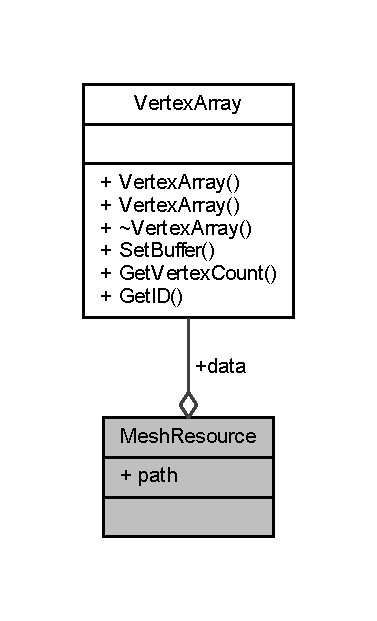
\includegraphics[width=181pt]{struct_mesh_resource__coll__graph}
\end{center}
\end{figure}
\subsection*{Public Attributes}
\begin{DoxyCompactItemize}
\item 
std\+::string \mbox{\hyperlink{struct_mesh_resource_a614a05a4784b5ab50bedbc676ff5b9a8}{path}}
\item 
\mbox{\hyperlink{class_vertex_array}{Vertex\+Array}} \mbox{\hyperlink{struct_mesh_resource_a755374f1f315a283e3bd1aa1d29d3a0a}{data}}
\end{DoxyCompactItemize}


\subsection{Member Data Documentation}
\mbox{\Hypertarget{struct_mesh_resource_a755374f1f315a283e3bd1aa1d29d3a0a}\label{struct_mesh_resource_a755374f1f315a283e3bd1aa1d29d3a0a}} 
\index{Mesh\+Resource@{Mesh\+Resource}!data@{data}}
\index{data@{data}!Mesh\+Resource@{Mesh\+Resource}}
\subsubsection{\texorpdfstring{data}{data}}
{\footnotesize\ttfamily \mbox{\hyperlink{class_vertex_array}{Vertex\+Array}} Mesh\+Resource\+::data}

\mbox{\Hypertarget{struct_mesh_resource_a614a05a4784b5ab50bedbc676ff5b9a8}\label{struct_mesh_resource_a614a05a4784b5ab50bedbc676ff5b9a8}} 
\index{Mesh\+Resource@{Mesh\+Resource}!path@{path}}
\index{path@{path}!Mesh\+Resource@{Mesh\+Resource}}
\subsubsection{\texorpdfstring{path}{path}}
{\footnotesize\ttfamily std\+::string Mesh\+Resource\+::path}



The documentation for this struct was generated from the following file\+:\begin{DoxyCompactItemize}
\item 
\mbox{\hyperlink{_resources_8h}{Resources.\+h}}\end{DoxyCompactItemize}

\hypertarget{class_mouse_handler}{}\section{Mouse\+Handler Class Reference}
\label{class_mouse_handler}\index{Mouse\+Handler@{Mouse\+Handler}}


{\ttfamily \#include $<$Mouse\+Handler.\+h$>$}



Collaboration diagram for Mouse\+Handler\+:
\nopagebreak
\begin{figure}[H]
\begin{center}
\leavevmode
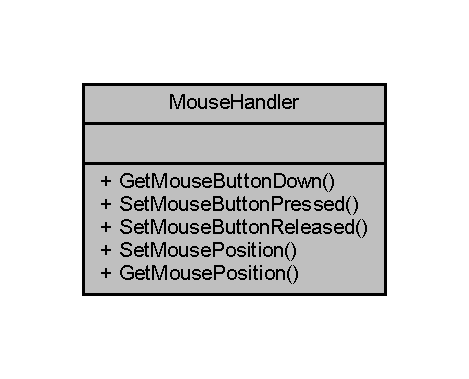
\includegraphics[width=225pt]{class_mouse_handler__coll__graph}
\end{center}
\end{figure}
\subsection*{Public Member Functions}
\begin{DoxyCompactItemize}
\item 
bool \mbox{\hyperlink{class_mouse_handler_a20fc955fca9c7a4b8c621b95270df0e7}{Get\+Mouse\+Button\+Down}} (int \+\_\+button)
\item 
void \mbox{\hyperlink{class_mouse_handler_a0572e9d8c3993813e4e91905cd64b6d3}{Set\+Mouse\+Button\+Pressed}} (S\+D\+L\+\_\+\+Mouse\+Button\+Event \+\_\+event)
\item 
void \mbox{\hyperlink{class_mouse_handler_a87c9624aabb7e7377dbf4c2eea544bee}{Set\+Mouse\+Button\+Released}} (S\+D\+L\+\_\+\+Mouse\+Button\+Event \+\_\+event)
\item 
void \mbox{\hyperlink{class_mouse_handler_a6b21ab3506b8bd90043f887ec43d93e2}{Set\+Mouse\+Position}} (int \+\_\+x, int \+\_\+y)
\item 
glm\+::vec2 \mbox{\hyperlink{class_mouse_handler_ad845f8049b6a4b22dc337943ba13726e}{Get\+Mouse\+Position}} ()
\end{DoxyCompactItemize}


\subsection{Member Function Documentation}
\mbox{\Hypertarget{class_mouse_handler_a20fc955fca9c7a4b8c621b95270df0e7}\label{class_mouse_handler_a20fc955fca9c7a4b8c621b95270df0e7}} 
\index{Mouse\+Handler@{Mouse\+Handler}!Get\+Mouse\+Button\+Down@{Get\+Mouse\+Button\+Down}}
\index{Get\+Mouse\+Button\+Down@{Get\+Mouse\+Button\+Down}!Mouse\+Handler@{Mouse\+Handler}}
\subsubsection{\texorpdfstring{Get\+Mouse\+Button\+Down()}{GetMouseButtonDown()}}
{\footnotesize\ttfamily bool Mouse\+Handler\+::\+Get\+Mouse\+Button\+Down (\begin{DoxyParamCaption}\item[{int}]{\+\_\+button }\end{DoxyParamCaption})}

\mbox{\Hypertarget{class_mouse_handler_ad845f8049b6a4b22dc337943ba13726e}\label{class_mouse_handler_ad845f8049b6a4b22dc337943ba13726e}} 
\index{Mouse\+Handler@{Mouse\+Handler}!Get\+Mouse\+Position@{Get\+Mouse\+Position}}
\index{Get\+Mouse\+Position@{Get\+Mouse\+Position}!Mouse\+Handler@{Mouse\+Handler}}
\subsubsection{\texorpdfstring{Get\+Mouse\+Position()}{GetMousePosition()}}
{\footnotesize\ttfamily glm\+::vec2 Mouse\+Handler\+::\+Get\+Mouse\+Position (\begin{DoxyParamCaption}{ }\end{DoxyParamCaption})\hspace{0.3cm}{\ttfamily [inline]}}

\mbox{\Hypertarget{class_mouse_handler_a0572e9d8c3993813e4e91905cd64b6d3}\label{class_mouse_handler_a0572e9d8c3993813e4e91905cd64b6d3}} 
\index{Mouse\+Handler@{Mouse\+Handler}!Set\+Mouse\+Button\+Pressed@{Set\+Mouse\+Button\+Pressed}}
\index{Set\+Mouse\+Button\+Pressed@{Set\+Mouse\+Button\+Pressed}!Mouse\+Handler@{Mouse\+Handler}}
\subsubsection{\texorpdfstring{Set\+Mouse\+Button\+Pressed()}{SetMouseButtonPressed()}}
{\footnotesize\ttfamily void Mouse\+Handler\+::\+Set\+Mouse\+Button\+Pressed (\begin{DoxyParamCaption}\item[{S\+D\+L\+\_\+\+Mouse\+Button\+Event}]{\+\_\+event }\end{DoxyParamCaption})}

\mbox{\Hypertarget{class_mouse_handler_a87c9624aabb7e7377dbf4c2eea544bee}\label{class_mouse_handler_a87c9624aabb7e7377dbf4c2eea544bee}} 
\index{Mouse\+Handler@{Mouse\+Handler}!Set\+Mouse\+Button\+Released@{Set\+Mouse\+Button\+Released}}
\index{Set\+Mouse\+Button\+Released@{Set\+Mouse\+Button\+Released}!Mouse\+Handler@{Mouse\+Handler}}
\subsubsection{\texorpdfstring{Set\+Mouse\+Button\+Released()}{SetMouseButtonReleased()}}
{\footnotesize\ttfamily void Mouse\+Handler\+::\+Set\+Mouse\+Button\+Released (\begin{DoxyParamCaption}\item[{S\+D\+L\+\_\+\+Mouse\+Button\+Event}]{\+\_\+event }\end{DoxyParamCaption})}

\mbox{\Hypertarget{class_mouse_handler_a6b21ab3506b8bd90043f887ec43d93e2}\label{class_mouse_handler_a6b21ab3506b8bd90043f887ec43d93e2}} 
\index{Mouse\+Handler@{Mouse\+Handler}!Set\+Mouse\+Position@{Set\+Mouse\+Position}}
\index{Set\+Mouse\+Position@{Set\+Mouse\+Position}!Mouse\+Handler@{Mouse\+Handler}}
\subsubsection{\texorpdfstring{Set\+Mouse\+Position()}{SetMousePosition()}}
{\footnotesize\ttfamily void Mouse\+Handler\+::\+Set\+Mouse\+Position (\begin{DoxyParamCaption}\item[{int}]{\+\_\+x,  }\item[{int}]{\+\_\+y }\end{DoxyParamCaption})}



The documentation for this class was generated from the following files\+:\begin{DoxyCompactItemize}
\item 
\mbox{\hyperlink{_mouse_handler_8h}{Mouse\+Handler.\+h}}\item 
\mbox{\hyperlink{_mouse_handler_8cpp}{Mouse\+Handler.\+cpp}}\end{DoxyCompactItemize}

\hypertarget{class_orthagraphic}{}\section{Orthagraphic Class Reference}
\label{class_orthagraphic}\index{Orthagraphic@{Orthagraphic}}


{\ttfamily \#include $<$Orthagraphic.\+h$>$}



Inheritance diagram for Orthagraphic\+:
\nopagebreak
\begin{figure}[H]
\begin{center}
\leavevmode
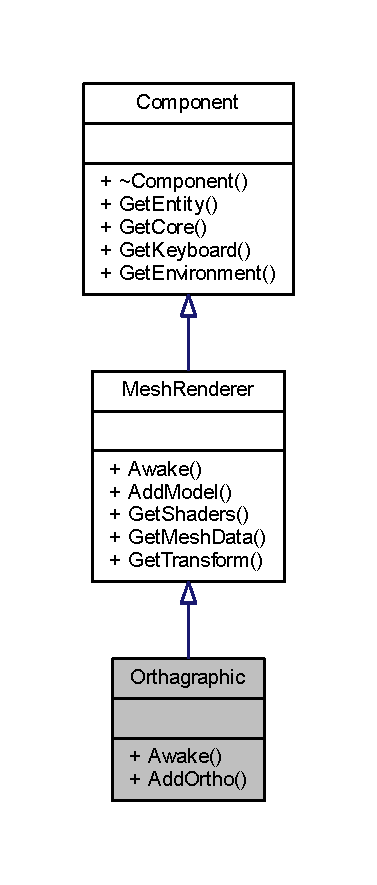
\includegraphics[width=181pt]{class_orthagraphic__inherit__graph}
\end{center}
\end{figure}


Collaboration diagram for Orthagraphic\+:
\nopagebreak
\begin{figure}[H]
\begin{center}
\leavevmode
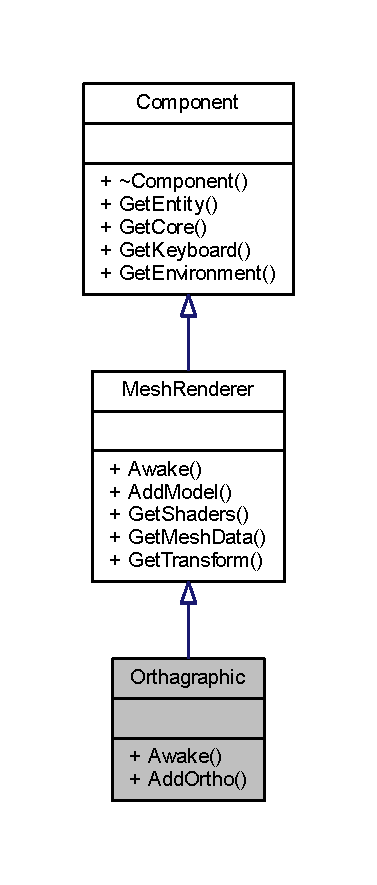
\includegraphics[width=181pt]{class_orthagraphic__coll__graph}
\end{center}
\end{figure}
\subsection*{Public Member Functions}
\begin{DoxyCompactItemize}
\item 
virtual void \mbox{\hyperlink{class_orthagraphic_a62f9d1b5d54623252bc3d15eba1e7181}{Awake}} ()
\item 
void \mbox{\hyperlink{class_orthagraphic_a7566bfec317c25a115d4d0b7debfb36c}{Add\+Ortho}} (std\+::string \+\_\+model\+Path, std\+::string \+\_\+vertex\+Path, std\+::string \+\_\+frag\+Path)
\end{DoxyCompactItemize}


\subsection{Member Function Documentation}
\mbox{\Hypertarget{class_orthagraphic_a7566bfec317c25a115d4d0b7debfb36c}\label{class_orthagraphic_a7566bfec317c25a115d4d0b7debfb36c}} 
\index{Orthagraphic@{Orthagraphic}!Add\+Ortho@{Add\+Ortho}}
\index{Add\+Ortho@{Add\+Ortho}!Orthagraphic@{Orthagraphic}}
\subsubsection{\texorpdfstring{Add\+Ortho()}{AddOrtho()}}
{\footnotesize\ttfamily void Orthagraphic\+::\+Add\+Ortho (\begin{DoxyParamCaption}\item[{std\+::string}]{\+\_\+model\+Path,  }\item[{std\+::string}]{\+\_\+vertex\+Path,  }\item[{std\+::string}]{\+\_\+frag\+Path }\end{DoxyParamCaption})}

Here is the call graph for this function\+:
\nopagebreak
\begin{figure}[H]
\begin{center}
\leavevmode
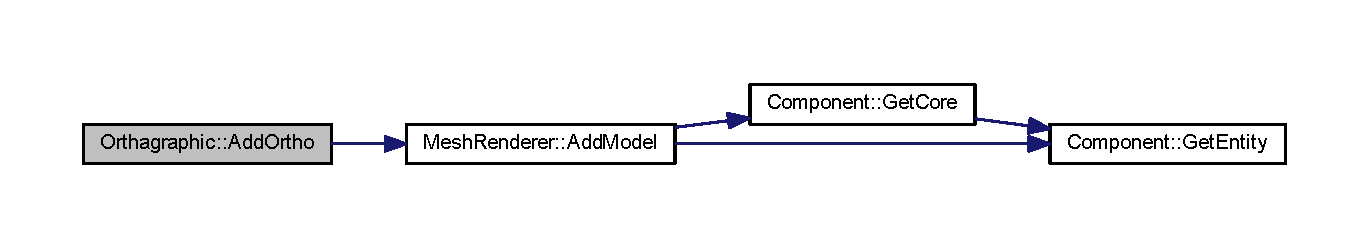
\includegraphics[width=350pt]{class_orthagraphic_a7566bfec317c25a115d4d0b7debfb36c_cgraph}
\end{center}
\end{figure}
\mbox{\Hypertarget{class_orthagraphic_a62f9d1b5d54623252bc3d15eba1e7181}\label{class_orthagraphic_a62f9d1b5d54623252bc3d15eba1e7181}} 
\index{Orthagraphic@{Orthagraphic}!Awake@{Awake}}
\index{Awake@{Awake}!Orthagraphic@{Orthagraphic}}
\subsubsection{\texorpdfstring{Awake()}{Awake()}}
{\footnotesize\ttfamily void Orthagraphic\+::\+Awake (\begin{DoxyParamCaption}{ }\end{DoxyParamCaption})\hspace{0.3cm}{\ttfamily [virtual]}}



Reimplemented from \mbox{\hyperlink{class_mesh_renderer_a3fc0e9658d3b9a53e3559cb9b939aeb9}{Mesh\+Renderer}}.

Here is the call graph for this function\+:
\nopagebreak
\begin{figure}[H]
\begin{center}
\leavevmode
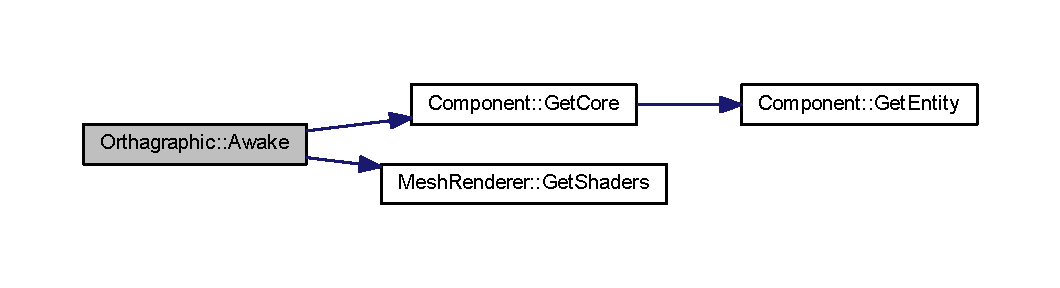
\includegraphics[width=350pt]{class_orthagraphic_a62f9d1b5d54623252bc3d15eba1e7181_cgraph}
\end{center}
\end{figure}


The documentation for this class was generated from the following files\+:\begin{DoxyCompactItemize}
\item 
\mbox{\hyperlink{_orthagraphic_8h}{Orthagraphic.\+h}}\item 
\mbox{\hyperlink{_orthagraphic_8cpp}{Orthagraphic.\+cpp}}\end{DoxyCompactItemize}

\hypertarget{class_resources}{}\section{Resources Class Reference}
\label{class_resources}\index{Resources@{Resources}}


{\ttfamily \#include $<$Resources.\+h$>$}



Collaboration diagram for Resources\+:
\nopagebreak
\begin{figure}[H]
\begin{center}
\leavevmode
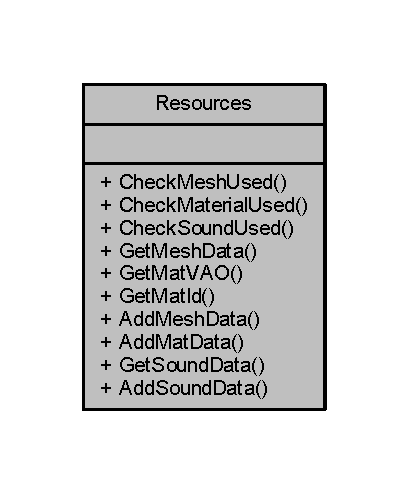
\includegraphics[width=196pt]{class_resources__coll__graph}
\end{center}
\end{figure}
\subsection*{Public Member Functions}
\begin{DoxyCompactItemize}
\item 
bool \mbox{\hyperlink{class_resources_a95b7267455d6a92af4b7525317e6fda2}{Check\+Mesh\+Used}} (std\+::string \+\_\+path)
\item 
bool \mbox{\hyperlink{class_resources_a7fa1d49c4fa656c355547235687f7cf2}{Check\+Material\+Used}} (std\+::string \+\_\+path)
\item 
bool \mbox{\hyperlink{class_resources_a7c9a86ab08c2e391771efec6570a55e3}{Check\+Sound\+Used}} (std\+::string \+\_\+path)
\item 
std\+::shared\+\_\+ptr$<$ \mbox{\hyperlink{class_vertex_array}{Vertex\+Array}} $>$ \mbox{\hyperlink{class_resources_adf647cccbff04491447ef4ccb262e2de}{Get\+Mesh\+Data}} (std\+::string \+\_\+path)
\item 
std\+::shared\+\_\+ptr$<$ \mbox{\hyperlink{class_vertex_array}{Vertex\+Array}} $>$ \mbox{\hyperlink{class_resources_a8225551fdeddbf2b6f34d44323f7333e}{Get\+Mat\+V\+AO}} (std\+::string \+\_\+path)
\item 
G\+Luint \mbox{\hyperlink{class_resources_a337663d0deaccb636135494a42400b52}{Get\+Mat\+Id}} (std\+::string \+\_\+path)
\item 
void \mbox{\hyperlink{class_resources_a44d04fc717db8de2e1e402e2927f99ff}{Add\+Mesh\+Data}} (std\+::shared\+\_\+ptr$<$ \mbox{\hyperlink{class_vertex_array}{Vertex\+Array}} $>$ \+\_\+data, std\+::string \+\_\+path)
\item 
void \mbox{\hyperlink{class_resources_a960db51890620adeb83f2a2c30b40af9}{Add\+Mat\+Data}} (std\+::string \+\_\+path, std\+::shared\+\_\+ptr$<$ \mbox{\hyperlink{class_vertex_array}{Vertex\+Array}} $>$ \+\_\+\+V\+AO, G\+Luint \+\_\+id)
\item 
std\+::shared\+\_\+ptr$<$ \mbox{\hyperlink{class_vertex_array}{Vertex\+Array}} $>$ \mbox{\hyperlink{class_resources_a163cbc0337f5262b19098766d85196a1}{Get\+Sound\+Data}} ()
\item 
void \mbox{\hyperlink{class_resources_a178691b808af645c7642b4bf4915ceba}{Add\+Sound\+Data}} (std\+::shared\+\_\+ptr$<$ \mbox{\hyperlink{class_vertex_array}{Vertex\+Array}} $>$ \+\_\+data, std\+::string \+\_\+path)
\end{DoxyCompactItemize}


\subsection{Member Function Documentation}
\mbox{\Hypertarget{class_resources_a960db51890620adeb83f2a2c30b40af9}\label{class_resources_a960db51890620adeb83f2a2c30b40af9}} 
\index{Resources@{Resources}!Add\+Mat\+Data@{Add\+Mat\+Data}}
\index{Add\+Mat\+Data@{Add\+Mat\+Data}!Resources@{Resources}}
\subsubsection{\texorpdfstring{Add\+Mat\+Data()}{AddMatData()}}
{\footnotesize\ttfamily void Resources\+::\+Add\+Mat\+Data (\begin{DoxyParamCaption}\item[{std\+::string}]{\+\_\+path,  }\item[{std\+::shared\+\_\+ptr$<$ \mbox{\hyperlink{class_vertex_array}{Vertex\+Array}} $>$}]{\+\_\+\+V\+AO,  }\item[{G\+Luint}]{\+\_\+id }\end{DoxyParamCaption})}

\mbox{\Hypertarget{class_resources_a44d04fc717db8de2e1e402e2927f99ff}\label{class_resources_a44d04fc717db8de2e1e402e2927f99ff}} 
\index{Resources@{Resources}!Add\+Mesh\+Data@{Add\+Mesh\+Data}}
\index{Add\+Mesh\+Data@{Add\+Mesh\+Data}!Resources@{Resources}}
\subsubsection{\texorpdfstring{Add\+Mesh\+Data()}{AddMeshData()}}
{\footnotesize\ttfamily void Resources\+::\+Add\+Mesh\+Data (\begin{DoxyParamCaption}\item[{std\+::shared\+\_\+ptr$<$ \mbox{\hyperlink{class_vertex_array}{Vertex\+Array}} $>$}]{\+\_\+data,  }\item[{std\+::string}]{\+\_\+path }\end{DoxyParamCaption})}

\mbox{\Hypertarget{class_resources_a178691b808af645c7642b4bf4915ceba}\label{class_resources_a178691b808af645c7642b4bf4915ceba}} 
\index{Resources@{Resources}!Add\+Sound\+Data@{Add\+Sound\+Data}}
\index{Add\+Sound\+Data@{Add\+Sound\+Data}!Resources@{Resources}}
\subsubsection{\texorpdfstring{Add\+Sound\+Data()}{AddSoundData()}}
{\footnotesize\ttfamily void Resources\+::\+Add\+Sound\+Data (\begin{DoxyParamCaption}\item[{std\+::shared\+\_\+ptr$<$ \mbox{\hyperlink{class_vertex_array}{Vertex\+Array}} $>$}]{\+\_\+data,  }\item[{std\+::string}]{\+\_\+path }\end{DoxyParamCaption})}

\mbox{\Hypertarget{class_resources_a7fa1d49c4fa656c355547235687f7cf2}\label{class_resources_a7fa1d49c4fa656c355547235687f7cf2}} 
\index{Resources@{Resources}!Check\+Material\+Used@{Check\+Material\+Used}}
\index{Check\+Material\+Used@{Check\+Material\+Used}!Resources@{Resources}}
\subsubsection{\texorpdfstring{Check\+Material\+Used()}{CheckMaterialUsed()}}
{\footnotesize\ttfamily bool Resources\+::\+Check\+Material\+Used (\begin{DoxyParamCaption}\item[{std\+::string}]{\+\_\+path }\end{DoxyParamCaption})}

\mbox{\Hypertarget{class_resources_a95b7267455d6a92af4b7525317e6fda2}\label{class_resources_a95b7267455d6a92af4b7525317e6fda2}} 
\index{Resources@{Resources}!Check\+Mesh\+Used@{Check\+Mesh\+Used}}
\index{Check\+Mesh\+Used@{Check\+Mesh\+Used}!Resources@{Resources}}
\subsubsection{\texorpdfstring{Check\+Mesh\+Used()}{CheckMeshUsed()}}
{\footnotesize\ttfamily bool Resources\+::\+Check\+Mesh\+Used (\begin{DoxyParamCaption}\item[{std\+::string}]{\+\_\+path }\end{DoxyParamCaption})}

\mbox{\Hypertarget{class_resources_a7c9a86ab08c2e391771efec6570a55e3}\label{class_resources_a7c9a86ab08c2e391771efec6570a55e3}} 
\index{Resources@{Resources}!Check\+Sound\+Used@{Check\+Sound\+Used}}
\index{Check\+Sound\+Used@{Check\+Sound\+Used}!Resources@{Resources}}
\subsubsection{\texorpdfstring{Check\+Sound\+Used()}{CheckSoundUsed()}}
{\footnotesize\ttfamily bool Resources\+::\+Check\+Sound\+Used (\begin{DoxyParamCaption}\item[{std\+::string}]{\+\_\+path }\end{DoxyParamCaption})}

\mbox{\Hypertarget{class_resources_a337663d0deaccb636135494a42400b52}\label{class_resources_a337663d0deaccb636135494a42400b52}} 
\index{Resources@{Resources}!Get\+Mat\+Id@{Get\+Mat\+Id}}
\index{Get\+Mat\+Id@{Get\+Mat\+Id}!Resources@{Resources}}
\subsubsection{\texorpdfstring{Get\+Mat\+Id()}{GetMatId()}}
{\footnotesize\ttfamily G\+Luint Resources\+::\+Get\+Mat\+Id (\begin{DoxyParamCaption}\item[{std\+::string}]{\+\_\+path }\end{DoxyParamCaption})}

\mbox{\Hypertarget{class_resources_a8225551fdeddbf2b6f34d44323f7333e}\label{class_resources_a8225551fdeddbf2b6f34d44323f7333e}} 
\index{Resources@{Resources}!Get\+Mat\+V\+AO@{Get\+Mat\+V\+AO}}
\index{Get\+Mat\+V\+AO@{Get\+Mat\+V\+AO}!Resources@{Resources}}
\subsubsection{\texorpdfstring{Get\+Mat\+V\+A\+O()}{GetMatVAO()}}
{\footnotesize\ttfamily std\+::shared\+\_\+ptr$<$ \mbox{\hyperlink{class_vertex_array}{Vertex\+Array}} $>$ Resources\+::\+Get\+Mat\+V\+AO (\begin{DoxyParamCaption}\item[{std\+::string}]{\+\_\+path }\end{DoxyParamCaption})}

\mbox{\Hypertarget{class_resources_adf647cccbff04491447ef4ccb262e2de}\label{class_resources_adf647cccbff04491447ef4ccb262e2de}} 
\index{Resources@{Resources}!Get\+Mesh\+Data@{Get\+Mesh\+Data}}
\index{Get\+Mesh\+Data@{Get\+Mesh\+Data}!Resources@{Resources}}
\subsubsection{\texorpdfstring{Get\+Mesh\+Data()}{GetMeshData()}}
{\footnotesize\ttfamily std\+::shared\+\_\+ptr$<$ \mbox{\hyperlink{class_vertex_array}{Vertex\+Array}} $>$ Resources\+::\+Get\+Mesh\+Data (\begin{DoxyParamCaption}\item[{std\+::string}]{\+\_\+path }\end{DoxyParamCaption})}

\mbox{\Hypertarget{class_resources_a163cbc0337f5262b19098766d85196a1}\label{class_resources_a163cbc0337f5262b19098766d85196a1}} 
\index{Resources@{Resources}!Get\+Sound\+Data@{Get\+Sound\+Data}}
\index{Get\+Sound\+Data@{Get\+Sound\+Data}!Resources@{Resources}}
\subsubsection{\texorpdfstring{Get\+Sound\+Data()}{GetSoundData()}}
{\footnotesize\ttfamily std\+::shared\+\_\+ptr$<$ \mbox{\hyperlink{class_vertex_array}{Vertex\+Array}} $>$ Resources\+::\+Get\+Sound\+Data (\begin{DoxyParamCaption}{ }\end{DoxyParamCaption})}



The documentation for this class was generated from the following files\+:\begin{DoxyCompactItemize}
\item 
\mbox{\hyperlink{_resources_8h}{Resources.\+h}}\item 
\mbox{\hyperlink{_resources_8cpp}{Resources.\+cpp}}\end{DoxyCompactItemize}

\hypertarget{class_screen}{}\section{Screen Class Reference}
\label{class_screen}\index{Screen@{Screen}}


{\ttfamily \#include $<$Screen.\+h$>$}



Collaboration diagram for Screen\+:
\nopagebreak
\begin{figure}[H]
\begin{center}
\leavevmode
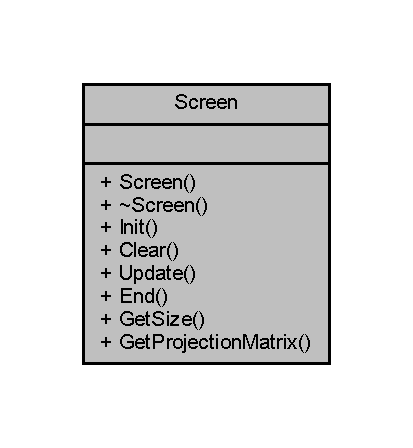
\includegraphics[width=198pt]{class_screen__coll__graph}
\end{center}
\end{figure}
\subsection*{Public Member Functions}
\begin{DoxyCompactItemize}
\item 
\mbox{\hyperlink{class_screen_ae7576476fc6e6a6eaa66389fdc41fe72}{Screen}} ()
\item 
\mbox{\hyperlink{class_screen_a4243bc17596af96415b09ac48205676d}{$\sim$\+Screen}} ()
\item 
void \mbox{\hyperlink{class_screen_a2da4b3a4b37151b4f0ac1e9d3c189d10}{Init}} ()
\item 
void \mbox{\hyperlink{class_screen_aef2c4e4e116cc5d1321392545cba6caa}{Clear}} ()
\item 
void \mbox{\hyperlink{class_screen_a022bd9b551faa54312ef867267865ec7}{Update}} ()
\item 
void \mbox{\hyperlink{class_screen_af1db8b519ceea7831567c8a1e59ff6f7}{End}} ()
\item 
glm\+::vec2 \mbox{\hyperlink{class_screen_a2b2783809f44b124f19b45fbd0c21241}{Get\+Size}} ()
\item 
glm\+::mat4 \mbox{\hyperlink{class_screen_ad43c28bb9ccca3ef351dfd4d9f347fb0}{Get\+Projection\+Matrix}} ()
\end{DoxyCompactItemize}


\subsection{Constructor \& Destructor Documentation}
\mbox{\Hypertarget{class_screen_ae7576476fc6e6a6eaa66389fdc41fe72}\label{class_screen_ae7576476fc6e6a6eaa66389fdc41fe72}} 
\index{Screen@{Screen}!Screen@{Screen}}
\index{Screen@{Screen}!Screen@{Screen}}
\subsubsection{\texorpdfstring{Screen()}{Screen()}}
{\footnotesize\ttfamily Screen\+::\+Screen (\begin{DoxyParamCaption}{ }\end{DoxyParamCaption})}

\mbox{\Hypertarget{class_screen_a4243bc17596af96415b09ac48205676d}\label{class_screen_a4243bc17596af96415b09ac48205676d}} 
\index{Screen@{Screen}!````~Screen@{$\sim$\+Screen}}
\index{````~Screen@{$\sim$\+Screen}!Screen@{Screen}}
\subsubsection{\texorpdfstring{$\sim$\+Screen()}{~Screen()}}
{\footnotesize\ttfamily Screen\+::$\sim$\+Screen (\begin{DoxyParamCaption}{ }\end{DoxyParamCaption})}



\subsection{Member Function Documentation}
\mbox{\Hypertarget{class_screen_aef2c4e4e116cc5d1321392545cba6caa}\label{class_screen_aef2c4e4e116cc5d1321392545cba6caa}} 
\index{Screen@{Screen}!Clear@{Clear}}
\index{Clear@{Clear}!Screen@{Screen}}
\subsubsection{\texorpdfstring{Clear()}{Clear()}}
{\footnotesize\ttfamily void Screen\+::\+Clear (\begin{DoxyParamCaption}{ }\end{DoxyParamCaption})}

\mbox{\Hypertarget{class_screen_af1db8b519ceea7831567c8a1e59ff6f7}\label{class_screen_af1db8b519ceea7831567c8a1e59ff6f7}} 
\index{Screen@{Screen}!End@{End}}
\index{End@{End}!Screen@{Screen}}
\subsubsection{\texorpdfstring{End()}{End()}}
{\footnotesize\ttfamily void Screen\+::\+End (\begin{DoxyParamCaption}{ }\end{DoxyParamCaption})}

\mbox{\Hypertarget{class_screen_ad43c28bb9ccca3ef351dfd4d9f347fb0}\label{class_screen_ad43c28bb9ccca3ef351dfd4d9f347fb0}} 
\index{Screen@{Screen}!Get\+Projection\+Matrix@{Get\+Projection\+Matrix}}
\index{Get\+Projection\+Matrix@{Get\+Projection\+Matrix}!Screen@{Screen}}
\subsubsection{\texorpdfstring{Get\+Projection\+Matrix()}{GetProjectionMatrix()}}
{\footnotesize\ttfamily glm\+::mat4 Screen\+::\+Get\+Projection\+Matrix (\begin{DoxyParamCaption}{ }\end{DoxyParamCaption})\hspace{0.3cm}{\ttfamily [inline]}}

\mbox{\Hypertarget{class_screen_a2b2783809f44b124f19b45fbd0c21241}\label{class_screen_a2b2783809f44b124f19b45fbd0c21241}} 
\index{Screen@{Screen}!Get\+Size@{Get\+Size}}
\index{Get\+Size@{Get\+Size}!Screen@{Screen}}
\subsubsection{\texorpdfstring{Get\+Size()}{GetSize()}}
{\footnotesize\ttfamily glm\+::vec2 Screen\+::\+Get\+Size (\begin{DoxyParamCaption}{ }\end{DoxyParamCaption})\hspace{0.3cm}{\ttfamily [inline]}}

\mbox{\Hypertarget{class_screen_a2da4b3a4b37151b4f0ac1e9d3c189d10}\label{class_screen_a2da4b3a4b37151b4f0ac1e9d3c189d10}} 
\index{Screen@{Screen}!Init@{Init}}
\index{Init@{Init}!Screen@{Screen}}
\subsubsection{\texorpdfstring{Init()}{Init()}}
{\footnotesize\ttfamily void Screen\+::\+Init (\begin{DoxyParamCaption}{ }\end{DoxyParamCaption})}

\mbox{\Hypertarget{class_screen_a022bd9b551faa54312ef867267865ec7}\label{class_screen_a022bd9b551faa54312ef867267865ec7}} 
\index{Screen@{Screen}!Update@{Update}}
\index{Update@{Update}!Screen@{Screen}}
\subsubsection{\texorpdfstring{Update()}{Update()}}
{\footnotesize\ttfamily void Screen\+::\+Update (\begin{DoxyParamCaption}{ }\end{DoxyParamCaption})}



The documentation for this class was generated from the following files\+:\begin{DoxyCompactItemize}
\item 
\mbox{\hyperlink{_screen_8h}{Screen.\+h}}\item 
\mbox{\hyperlink{_screen_8cpp}{Screen.\+cpp}}\end{DoxyCompactItemize}

\hypertarget{class_shader_program}{}\section{Shader\+Program Class Reference}
\label{class_shader_program}\index{Shader\+Program@{Shader\+Program}}


{\ttfamily \#include $<$Shader\+Program.\+h$>$}



Collaboration diagram for Shader\+Program\+:
\nopagebreak
\begin{figure}[H]
\begin{center}
\leavevmode
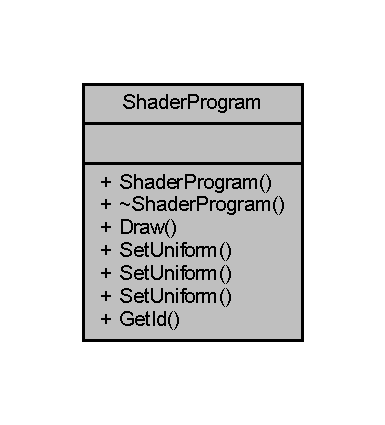
\includegraphics[width=185pt]{class_shader_program__coll__graph}
\end{center}
\end{figure}
\subsection*{Public Member Functions}
\begin{DoxyCompactItemize}
\item 
\mbox{\hyperlink{class_shader_program_a835418de83ffd318d244286f9b1786d1}{Shader\+Program}} (std\+::string \+\_\+vert, std\+::string \+\_\+frag)
\item 
\mbox{\hyperlink{class_shader_program_a2d2eadcfc48cc2e2ddb82aba70553a9f}{$\sim$\+Shader\+Program}} ()
\item 
void \mbox{\hyperlink{class_shader_program_aca655dd6fd3034c99d01b7627789087f}{Draw}} (\mbox{\hyperlink{class_vertex_array}{Vertex\+Array}} \&\+\_\+vertex\+Array)
\item 
void \mbox{\hyperlink{class_shader_program_a415d4a54caef8913771ebce26478291c}{Set\+Uniform}} (std\+::string \+\_\+uniform, glm\+::vec4 \+\_\+value)
\item 
void \mbox{\hyperlink{class_shader_program_a6b964df4ebf8b6258ee1989e463d9a9b}{Set\+Uniform}} (std\+::string \+\_\+uniform, float \+\_\+value)
\item 
void \mbox{\hyperlink{class_shader_program_acf22820261bc06136eee4ece975fb164}{Set\+Uniform}} (std\+::string \+\_\+uniform, glm\+::mat4 \+\_\+value)
\item 
G\+Luint \mbox{\hyperlink{class_shader_program_a5b2653f0b69e26a9b867b1a7a3aec2ef}{Get\+Id}} ()
\end{DoxyCompactItemize}


\subsection{Constructor \& Destructor Documentation}
\mbox{\Hypertarget{class_shader_program_a835418de83ffd318d244286f9b1786d1}\label{class_shader_program_a835418de83ffd318d244286f9b1786d1}} 
\index{Shader\+Program@{Shader\+Program}!Shader\+Program@{Shader\+Program}}
\index{Shader\+Program@{Shader\+Program}!Shader\+Program@{Shader\+Program}}
\subsubsection{\texorpdfstring{Shader\+Program()}{ShaderProgram()}}
{\footnotesize\ttfamily Shader\+Program\+::\+Shader\+Program (\begin{DoxyParamCaption}\item[{std\+::string}]{\+\_\+vert,  }\item[{std\+::string}]{\+\_\+frag }\end{DoxyParamCaption})}

\mbox{\Hypertarget{class_shader_program_a2d2eadcfc48cc2e2ddb82aba70553a9f}\label{class_shader_program_a2d2eadcfc48cc2e2ddb82aba70553a9f}} 
\index{Shader\+Program@{Shader\+Program}!````~Shader\+Program@{$\sim$\+Shader\+Program}}
\index{````~Shader\+Program@{$\sim$\+Shader\+Program}!Shader\+Program@{Shader\+Program}}
\subsubsection{\texorpdfstring{$\sim$\+Shader\+Program()}{~ShaderProgram()}}
{\footnotesize\ttfamily Shader\+Program\+::$\sim$\+Shader\+Program (\begin{DoxyParamCaption}{ }\end{DoxyParamCaption})}



\subsection{Member Function Documentation}
\mbox{\Hypertarget{class_shader_program_aca655dd6fd3034c99d01b7627789087f}\label{class_shader_program_aca655dd6fd3034c99d01b7627789087f}} 
\index{Shader\+Program@{Shader\+Program}!Draw@{Draw}}
\index{Draw@{Draw}!Shader\+Program@{Shader\+Program}}
\subsubsection{\texorpdfstring{Draw()}{Draw()}}
{\footnotesize\ttfamily void Shader\+Program\+::\+Draw (\begin{DoxyParamCaption}\item[{\mbox{\hyperlink{class_vertex_array}{Vertex\+Array}} \&}]{\+\_\+vertex\+Array }\end{DoxyParamCaption})}

Here is the call graph for this function\+:
\nopagebreak
\begin{figure}[H]
\begin{center}
\leavevmode
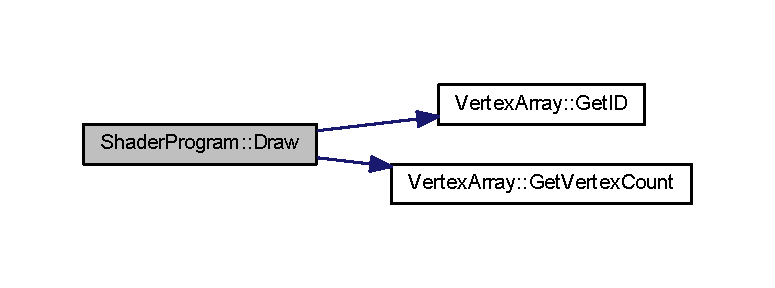
\includegraphics[width=350pt]{class_shader_program_aca655dd6fd3034c99d01b7627789087f_cgraph}
\end{center}
\end{figure}
\mbox{\Hypertarget{class_shader_program_a5b2653f0b69e26a9b867b1a7a3aec2ef}\label{class_shader_program_a5b2653f0b69e26a9b867b1a7a3aec2ef}} 
\index{Shader\+Program@{Shader\+Program}!Get\+Id@{Get\+Id}}
\index{Get\+Id@{Get\+Id}!Shader\+Program@{Shader\+Program}}
\subsubsection{\texorpdfstring{Get\+Id()}{GetId()}}
{\footnotesize\ttfamily G\+Luint Shader\+Program\+::\+Get\+Id (\begin{DoxyParamCaption}{ }\end{DoxyParamCaption})\hspace{0.3cm}{\ttfamily [inline]}}

\mbox{\Hypertarget{class_shader_program_a415d4a54caef8913771ebce26478291c}\label{class_shader_program_a415d4a54caef8913771ebce26478291c}} 
\index{Shader\+Program@{Shader\+Program}!Set\+Uniform@{Set\+Uniform}}
\index{Set\+Uniform@{Set\+Uniform}!Shader\+Program@{Shader\+Program}}
\subsubsection{\texorpdfstring{Set\+Uniform()}{SetUniform()}\hspace{0.1cm}{\footnotesize\ttfamily [1/3]}}
{\footnotesize\ttfamily void Shader\+Program\+::\+Set\+Uniform (\begin{DoxyParamCaption}\item[{std\+::string}]{\+\_\+uniform,  }\item[{glm\+::vec4}]{\+\_\+value }\end{DoxyParamCaption})}

\mbox{\Hypertarget{class_shader_program_a6b964df4ebf8b6258ee1989e463d9a9b}\label{class_shader_program_a6b964df4ebf8b6258ee1989e463d9a9b}} 
\index{Shader\+Program@{Shader\+Program}!Set\+Uniform@{Set\+Uniform}}
\index{Set\+Uniform@{Set\+Uniform}!Shader\+Program@{Shader\+Program}}
\subsubsection{\texorpdfstring{Set\+Uniform()}{SetUniform()}\hspace{0.1cm}{\footnotesize\ttfamily [2/3]}}
{\footnotesize\ttfamily void Shader\+Program\+::\+Set\+Uniform (\begin{DoxyParamCaption}\item[{std\+::string}]{\+\_\+uniform,  }\item[{float}]{\+\_\+value }\end{DoxyParamCaption})}

\mbox{\Hypertarget{class_shader_program_acf22820261bc06136eee4ece975fb164}\label{class_shader_program_acf22820261bc06136eee4ece975fb164}} 
\index{Shader\+Program@{Shader\+Program}!Set\+Uniform@{Set\+Uniform}}
\index{Set\+Uniform@{Set\+Uniform}!Shader\+Program@{Shader\+Program}}
\subsubsection{\texorpdfstring{Set\+Uniform()}{SetUniform()}\hspace{0.1cm}{\footnotesize\ttfamily [3/3]}}
{\footnotesize\ttfamily void Shader\+Program\+::\+Set\+Uniform (\begin{DoxyParamCaption}\item[{std\+::string}]{\+\_\+uniform,  }\item[{glm\+::mat4}]{\+\_\+value }\end{DoxyParamCaption})}



The documentation for this class was generated from the following files\+:\begin{DoxyCompactItemize}
\item 
\mbox{\hyperlink{_shader_program_8h}{Shader\+Program.\+h}}\item 
\mbox{\hyperlink{_shader_program_8cpp}{Shader\+Program.\+cpp}}\end{DoxyCompactItemize}

\hypertarget{class_sound}{}\section{Sound Class Reference}
\label{class_sound}\index{Sound@{Sound}}


{\ttfamily \#include $<$Sound.\+h$>$}



Collaboration diagram for Sound\+:
\nopagebreak
\begin{figure}[H]
\begin{center}
\leavevmode
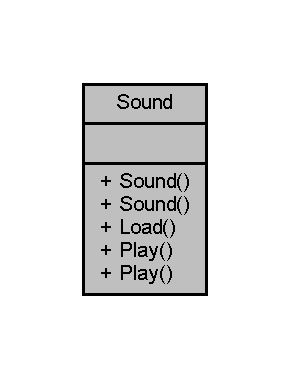
\includegraphics[width=139pt]{class_sound__coll__graph}
\end{center}
\end{figure}
\subsection*{Public Member Functions}
\begin{DoxyCompactItemize}
\item 
\mbox{\hyperlink{class_sound_a539c205cdf06fe2c621fd77c37bcfac9}{Sound}} ()
\item 
\mbox{\hyperlink{class_sound_ae588b8fb94e61912c7ecb5a3cea6f92d}{Sound}} (std\+::string \+\_\+file\+Path)
\item 
void \mbox{\hyperlink{class_sound_aa42f9f9625be20a1a84eeda8fac24cbb}{Load}} (std\+::string \+\_\+file\+Path)
\item 
void \mbox{\hyperlink{class_sound_a5ed28df22c2c96a5c40fa1d2444556d0}{Play}} (float \+\_\+volume, float \+\_\+var\+Min, float \+\_\+var\+Max)
\item 
void \mbox{\hyperlink{class_sound_a8106f65989f5cd4490c6cfe7032cf2b1}{Play}} ()
\end{DoxyCompactItemize}


\subsection{Constructor \& Destructor Documentation}
\mbox{\Hypertarget{class_sound_a539c205cdf06fe2c621fd77c37bcfac9}\label{class_sound_a539c205cdf06fe2c621fd77c37bcfac9}} 
\index{Sound@{Sound}!Sound@{Sound}}
\index{Sound@{Sound}!Sound@{Sound}}
\subsubsection{\texorpdfstring{Sound()}{Sound()}\hspace{0.1cm}{\footnotesize\ttfamily [1/2]}}
{\footnotesize\ttfamily Sound\+::\+Sound (\begin{DoxyParamCaption}{ }\end{DoxyParamCaption})}

\mbox{\Hypertarget{class_sound_ae588b8fb94e61912c7ecb5a3cea6f92d}\label{class_sound_ae588b8fb94e61912c7ecb5a3cea6f92d}} 
\index{Sound@{Sound}!Sound@{Sound}}
\index{Sound@{Sound}!Sound@{Sound}}
\subsubsection{\texorpdfstring{Sound()}{Sound()}\hspace{0.1cm}{\footnotesize\ttfamily [2/2]}}
{\footnotesize\ttfamily Sound\+::\+Sound (\begin{DoxyParamCaption}\item[{std\+::string}]{\+\_\+file\+Path }\end{DoxyParamCaption})}

Here is the call graph for this function\+:
\nopagebreak
\begin{figure}[H]
\begin{center}
\leavevmode
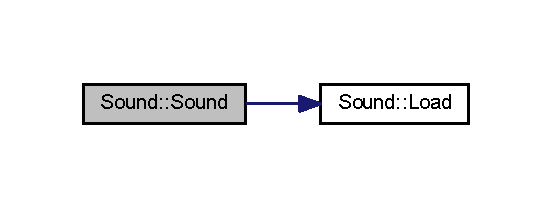
\includegraphics[width=265pt]{class_sound_ae588b8fb94e61912c7ecb5a3cea6f92d_cgraph}
\end{center}
\end{figure}


\subsection{Member Function Documentation}
\mbox{\Hypertarget{class_sound_aa42f9f9625be20a1a84eeda8fac24cbb}\label{class_sound_aa42f9f9625be20a1a84eeda8fac24cbb}} 
\index{Sound@{Sound}!Load@{Load}}
\index{Load@{Load}!Sound@{Sound}}
\subsubsection{\texorpdfstring{Load()}{Load()}}
{\footnotesize\ttfamily void Sound\+::\+Load (\begin{DoxyParamCaption}\item[{std\+::string}]{\+\_\+file\+Path }\end{DoxyParamCaption})}

Here is the caller graph for this function\+:
\nopagebreak
\begin{figure}[H]
\begin{center}
\leavevmode
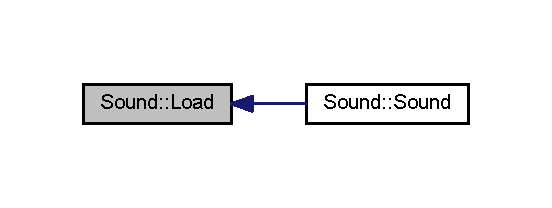
\includegraphics[width=265pt]{class_sound_aa42f9f9625be20a1a84eeda8fac24cbb_icgraph}
\end{center}
\end{figure}
\mbox{\Hypertarget{class_sound_a5ed28df22c2c96a5c40fa1d2444556d0}\label{class_sound_a5ed28df22c2c96a5c40fa1d2444556d0}} 
\index{Sound@{Sound}!Play@{Play}}
\index{Play@{Play}!Sound@{Sound}}
\subsubsection{\texorpdfstring{Play()}{Play()}\hspace{0.1cm}{\footnotesize\ttfamily [1/2]}}
{\footnotesize\ttfamily void Sound\+::\+Play (\begin{DoxyParamCaption}\item[{float}]{\+\_\+volume,  }\item[{float}]{\+\_\+var\+Min,  }\item[{float}]{\+\_\+var\+Max }\end{DoxyParamCaption})}

\mbox{\Hypertarget{class_sound_a8106f65989f5cd4490c6cfe7032cf2b1}\label{class_sound_a8106f65989f5cd4490c6cfe7032cf2b1}} 
\index{Sound@{Sound}!Play@{Play}}
\index{Play@{Play}!Sound@{Sound}}
\subsubsection{\texorpdfstring{Play()}{Play()}\hspace{0.1cm}{\footnotesize\ttfamily [2/2]}}
{\footnotesize\ttfamily void Sound\+::\+Play (\begin{DoxyParamCaption}{ }\end{DoxyParamCaption})}



The documentation for this class was generated from the following files\+:\begin{DoxyCompactItemize}
\item 
\mbox{\hyperlink{_sound_8h}{Sound.\+h}}\item 
\mbox{\hyperlink{_sound_8cpp}{Sound.\+cpp}}\end{DoxyCompactItemize}

\hypertarget{struct_sound_init}{}\section{Sound\+Init Struct Reference}
\label{struct_sound_init}\index{Sound\+Init@{Sound\+Init}}


Collaboration diagram for Sound\+Init\+:
\nopagebreak
\begin{figure}[H]
\begin{center}
\leavevmode
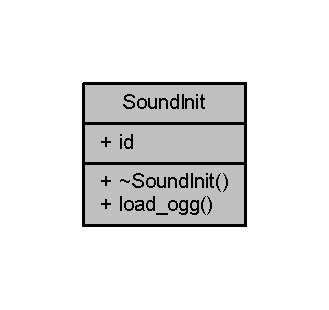
\includegraphics[width=158pt]{struct_sound_init__coll__graph}
\end{center}
\end{figure}
\subsection*{Public Member Functions}
\begin{DoxyCompactItemize}
\item 
\mbox{\hyperlink{struct_sound_init_a883a2ba69eda5faa5b405a383bab95ea}{$\sim$\+Sound\+Init}} ()
\item 
void \mbox{\hyperlink{struct_sound_init_adc9642cf26b528304eb9cd85bd178889}{load\+\_\+ogg}} (std\+::string \+\_\+file\+Path, std\+::vector$<$ char $>$ \&\+\_\+buffer, A\+Lenum \&\+\_\+format, A\+Lsizei \&\+\_\+freq)
\end{DoxyCompactItemize}
\subsection*{Public Attributes}
\begin{DoxyCompactItemize}
\item 
A\+Luint \mbox{\hyperlink{struct_sound_init_a1b59128bbf63c76a8bd40019b3090447}{id}}
\end{DoxyCompactItemize}


\subsection{Constructor \& Destructor Documentation}
\mbox{\Hypertarget{struct_sound_init_a883a2ba69eda5faa5b405a383bab95ea}\label{struct_sound_init_a883a2ba69eda5faa5b405a383bab95ea}} 
\index{Sound\+Init@{Sound\+Init}!````~Sound\+Init@{$\sim$\+Sound\+Init}}
\index{````~Sound\+Init@{$\sim$\+Sound\+Init}!Sound\+Init@{Sound\+Init}}
\subsubsection{\texorpdfstring{$\sim$\+Sound\+Init()}{~SoundInit()}}
{\footnotesize\ttfamily Sound\+Init\+::$\sim$\+Sound\+Init (\begin{DoxyParamCaption}{ }\end{DoxyParamCaption})\hspace{0.3cm}{\ttfamily [inline]}}



\subsection{Member Function Documentation}
\mbox{\Hypertarget{struct_sound_init_adc9642cf26b528304eb9cd85bd178889}\label{struct_sound_init_adc9642cf26b528304eb9cd85bd178889}} 
\index{Sound\+Init@{Sound\+Init}!load\+\_\+ogg@{load\+\_\+ogg}}
\index{load\+\_\+ogg@{load\+\_\+ogg}!Sound\+Init@{Sound\+Init}}
\subsubsection{\texorpdfstring{load\+\_\+ogg()}{load\_ogg()}}
{\footnotesize\ttfamily void Sound\+Init\+::load\+\_\+ogg (\begin{DoxyParamCaption}\item[{std\+::string}]{\+\_\+file\+Path,  }\item[{std\+::vector$<$ char $>$ \&}]{\+\_\+buffer,  }\item[{A\+Lenum \&}]{\+\_\+format,  }\item[{A\+Lsizei \&}]{\+\_\+freq }\end{DoxyParamCaption})\hspace{0.3cm}{\ttfamily [inline]}}



\subsection{Member Data Documentation}
\mbox{\Hypertarget{struct_sound_init_a1b59128bbf63c76a8bd40019b3090447}\label{struct_sound_init_a1b59128bbf63c76a8bd40019b3090447}} 
\index{Sound\+Init@{Sound\+Init}!id@{id}}
\index{id@{id}!Sound\+Init@{Sound\+Init}}
\subsubsection{\texorpdfstring{id}{id}}
{\footnotesize\ttfamily A\+Luint Sound\+Init\+::id}



The documentation for this struct was generated from the following file\+:\begin{DoxyCompactItemize}
\item 
\mbox{\hyperlink{_sound_8cpp}{Sound.\+cpp}}\end{DoxyCompactItemize}

\hypertarget{structstbi__io__callbacks}{}\section{stbi\+\_\+io\+\_\+callbacks Struct Reference}
\label{structstbi__io__callbacks}\index{stbi\+\_\+io\+\_\+callbacks@{stbi\+\_\+io\+\_\+callbacks}}


{\ttfamily \#include $<$stb\+\_\+image.\+h$>$}



Collaboration diagram for stbi\+\_\+io\+\_\+callbacks\+:
\nopagebreak
\begin{figure}[H]
\begin{center}
\leavevmode
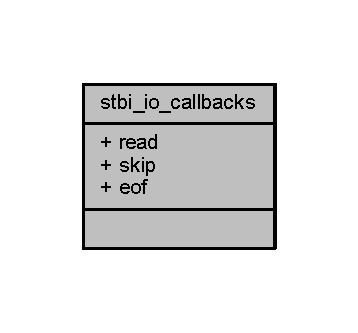
\includegraphics[width=172pt]{structstbi__io__callbacks__coll__graph}
\end{center}
\end{figure}
\subsection*{Public Attributes}
\begin{DoxyCompactItemize}
\item 
int($\ast$ \mbox{\hyperlink{structstbi__io__callbacks_a623e46b3a2a019611601409926283a88}{read}} )(void $\ast$user, char $\ast$data, int size)
\item 
void($\ast$ \mbox{\hyperlink{structstbi__io__callbacks_a257aac5480a90a6c4b8fbe86c1b01068}{skip}} )(void $\ast$user, int n)
\item 
int($\ast$ \mbox{\hyperlink{structstbi__io__callbacks_a319639db2f76e715eed7a7a974136832}{eof}} )(void $\ast$user)
\end{DoxyCompactItemize}


\subsection{Member Data Documentation}
\mbox{\Hypertarget{structstbi__io__callbacks_a319639db2f76e715eed7a7a974136832}\label{structstbi__io__callbacks_a319639db2f76e715eed7a7a974136832}} 
\index{stbi\+\_\+io\+\_\+callbacks@{stbi\+\_\+io\+\_\+callbacks}!eof@{eof}}
\index{eof@{eof}!stbi\+\_\+io\+\_\+callbacks@{stbi\+\_\+io\+\_\+callbacks}}
\subsubsection{\texorpdfstring{eof}{eof}}
{\footnotesize\ttfamily int($\ast$ stbi\+\_\+io\+\_\+callbacks\+::eof) (void $\ast$user)}

\mbox{\Hypertarget{structstbi__io__callbacks_a623e46b3a2a019611601409926283a88}\label{structstbi__io__callbacks_a623e46b3a2a019611601409926283a88}} 
\index{stbi\+\_\+io\+\_\+callbacks@{stbi\+\_\+io\+\_\+callbacks}!read@{read}}
\index{read@{read}!stbi\+\_\+io\+\_\+callbacks@{stbi\+\_\+io\+\_\+callbacks}}
\subsubsection{\texorpdfstring{read}{read}}
{\footnotesize\ttfamily int($\ast$ stbi\+\_\+io\+\_\+callbacks\+::read) (void $\ast$user, char $\ast$data, int size)}

\mbox{\Hypertarget{structstbi__io__callbacks_a257aac5480a90a6c4b8fbe86c1b01068}\label{structstbi__io__callbacks_a257aac5480a90a6c4b8fbe86c1b01068}} 
\index{stbi\+\_\+io\+\_\+callbacks@{stbi\+\_\+io\+\_\+callbacks}!skip@{skip}}
\index{skip@{skip}!stbi\+\_\+io\+\_\+callbacks@{stbi\+\_\+io\+\_\+callbacks}}
\subsubsection{\texorpdfstring{skip}{skip}}
{\footnotesize\ttfamily void($\ast$ stbi\+\_\+io\+\_\+callbacks\+::skip) (void $\ast$user, int n)}



The documentation for this struct was generated from the following file\+:\begin{DoxyCompactItemize}
\item 
\mbox{\hyperlink{stb__image_8h}{stb\+\_\+image.\+h}}\end{DoxyCompactItemize}

\hypertarget{class_transform}{}\section{Transform Class Reference}
\label{class_transform}\index{Transform@{Transform}}


{\ttfamily \#include $<$Transform.\+h$>$}



Inheritance diagram for Transform\+:
\nopagebreak
\begin{figure}[H]
\begin{center}
\leavevmode
\includegraphics[width=181pt]{class_transform__inherit__graph}
\end{center}
\end{figure}


Collaboration diagram for Transform\+:
\nopagebreak
\begin{figure}[H]
\begin{center}
\leavevmode
\includegraphics[width=181pt]{class_transform__coll__graph}
\end{center}
\end{figure}
\subsection*{Public Member Functions}
\begin{DoxyCompactItemize}
\item 
void \mbox{\hyperlink{class_transform_a82b79cb6c3af6ff717051144194d7e28}{Awake}} ()
\item 
void \mbox{\hyperlink{class_transform_af6c69e65b609a3d9e6028b4ffc7baada}{Set\+Transform}} (glm\+::vec3 \+\_\+position, float \+\_\+rotation, glm\+::vec3 \+\_\+scale)
\item 
void \mbox{\hyperlink{class_transform_ae6273120a938b99bbec52900770e6935}{Set\+Position}} (glm\+::vec3 \+\_\+position)
\item 
void \mbox{\hyperlink{class_transform_afee469d2dba032aab48471a0a0a42c5c}{Set\+Rotation}} (float \+\_\+rotation)
\item 
void \mbox{\hyperlink{class_transform_a8fb9524f56de0f31984d526156eec5cb}{Set\+Size}} (glm\+::vec2 \+\_\+size)
\item 
void \mbox{\hyperlink{class_transform_af741bc745e441e4c3175f9aff07c5d98}{Set\+Scale}} (glm\+::vec3 \+\_\+scale)
\item 
glm\+::vec3 \mbox{\hyperlink{class_transform_ab56d0806d3d2d67a0587c7ffebf0b2d0}{Get\+Position}} ()
\item 
float \mbox{\hyperlink{class_transform_aae910229b0e924b7bd2b7ead1a5ac1d3}{Get\+Rotation}} ()
\item 
glm\+::vec2 \mbox{\hyperlink{class_transform_a9042f2b38daaaf48b807b648e9adccbd}{Get\+Size}} ()
\item 
glm\+::vec3 \mbox{\hyperlink{class_transform_a28a37980813cba4e8bada11d5ee6d070}{Get\+Scale}} ()
\item 
glm\+::mat4 \mbox{\hyperlink{class_transform_aac5b8a016ec8ecb9eae51e636322a7dd}{Get\+Model\+Matrix}} ()
\end{DoxyCompactItemize}


\subsection{Member Function Documentation}
\mbox{\Hypertarget{class_transform_a82b79cb6c3af6ff717051144194d7e28}\label{class_transform_a82b79cb6c3af6ff717051144194d7e28}} 
\index{Transform@{Transform}!Awake@{Awake}}
\index{Awake@{Awake}!Transform@{Transform}}
\subsubsection{\texorpdfstring{Awake()}{Awake()}}
{\footnotesize\ttfamily void Transform\+::\+Awake (\begin{DoxyParamCaption}{ }\end{DoxyParamCaption})\hspace{0.3cm}{\ttfamily [virtual]}}



Reimplemented from \mbox{\hyperlink{class_component}{Component}}.

\mbox{\Hypertarget{class_transform_aac5b8a016ec8ecb9eae51e636322a7dd}\label{class_transform_aac5b8a016ec8ecb9eae51e636322a7dd}} 
\index{Transform@{Transform}!Get\+Model\+Matrix@{Get\+Model\+Matrix}}
\index{Get\+Model\+Matrix@{Get\+Model\+Matrix}!Transform@{Transform}}
\subsubsection{\texorpdfstring{Get\+Model\+Matrix()}{GetModelMatrix()}}
{\footnotesize\ttfamily glm\+::mat4 Transform\+::\+Get\+Model\+Matrix (\begin{DoxyParamCaption}{ }\end{DoxyParamCaption})}

\mbox{\Hypertarget{class_transform_ab56d0806d3d2d67a0587c7ffebf0b2d0}\label{class_transform_ab56d0806d3d2d67a0587c7ffebf0b2d0}} 
\index{Transform@{Transform}!Get\+Position@{Get\+Position}}
\index{Get\+Position@{Get\+Position}!Transform@{Transform}}
\subsubsection{\texorpdfstring{Get\+Position()}{GetPosition()}}
{\footnotesize\ttfamily glm\+::vec3 Transform\+::\+Get\+Position (\begin{DoxyParamCaption}{ }\end{DoxyParamCaption})\hspace{0.3cm}{\ttfamily [inline]}}

\mbox{\Hypertarget{class_transform_aae910229b0e924b7bd2b7ead1a5ac1d3}\label{class_transform_aae910229b0e924b7bd2b7ead1a5ac1d3}} 
\index{Transform@{Transform}!Get\+Rotation@{Get\+Rotation}}
\index{Get\+Rotation@{Get\+Rotation}!Transform@{Transform}}
\subsubsection{\texorpdfstring{Get\+Rotation()}{GetRotation()}}
{\footnotesize\ttfamily float Transform\+::\+Get\+Rotation (\begin{DoxyParamCaption}{ }\end{DoxyParamCaption})\hspace{0.3cm}{\ttfamily [inline]}}

\mbox{\Hypertarget{class_transform_a28a37980813cba4e8bada11d5ee6d070}\label{class_transform_a28a37980813cba4e8bada11d5ee6d070}} 
\index{Transform@{Transform}!Get\+Scale@{Get\+Scale}}
\index{Get\+Scale@{Get\+Scale}!Transform@{Transform}}
\subsubsection{\texorpdfstring{Get\+Scale()}{GetScale()}}
{\footnotesize\ttfamily glm\+::vec3 Transform\+::\+Get\+Scale (\begin{DoxyParamCaption}{ }\end{DoxyParamCaption})\hspace{0.3cm}{\ttfamily [inline]}}

\mbox{\Hypertarget{class_transform_a9042f2b38daaaf48b807b648e9adccbd}\label{class_transform_a9042f2b38daaaf48b807b648e9adccbd}} 
\index{Transform@{Transform}!Get\+Size@{Get\+Size}}
\index{Get\+Size@{Get\+Size}!Transform@{Transform}}
\subsubsection{\texorpdfstring{Get\+Size()}{GetSize()}}
{\footnotesize\ttfamily glm\+::vec2 Transform\+::\+Get\+Size (\begin{DoxyParamCaption}{ }\end{DoxyParamCaption})\hspace{0.3cm}{\ttfamily [inline]}}

\mbox{\Hypertarget{class_transform_ae6273120a938b99bbec52900770e6935}\label{class_transform_ae6273120a938b99bbec52900770e6935}} 
\index{Transform@{Transform}!Set\+Position@{Set\+Position}}
\index{Set\+Position@{Set\+Position}!Transform@{Transform}}
\subsubsection{\texorpdfstring{Set\+Position()}{SetPosition()}}
{\footnotesize\ttfamily void Transform\+::\+Set\+Position (\begin{DoxyParamCaption}\item[{glm\+::vec3}]{\+\_\+position }\end{DoxyParamCaption})}

\mbox{\Hypertarget{class_transform_afee469d2dba032aab48471a0a0a42c5c}\label{class_transform_afee469d2dba032aab48471a0a0a42c5c}} 
\index{Transform@{Transform}!Set\+Rotation@{Set\+Rotation}}
\index{Set\+Rotation@{Set\+Rotation}!Transform@{Transform}}
\subsubsection{\texorpdfstring{Set\+Rotation()}{SetRotation()}}
{\footnotesize\ttfamily void Transform\+::\+Set\+Rotation (\begin{DoxyParamCaption}\item[{float}]{\+\_\+rotation }\end{DoxyParamCaption})}

\mbox{\Hypertarget{class_transform_af741bc745e441e4c3175f9aff07c5d98}\label{class_transform_af741bc745e441e4c3175f9aff07c5d98}} 
\index{Transform@{Transform}!Set\+Scale@{Set\+Scale}}
\index{Set\+Scale@{Set\+Scale}!Transform@{Transform}}
\subsubsection{\texorpdfstring{Set\+Scale()}{SetScale()}}
{\footnotesize\ttfamily void Transform\+::\+Set\+Scale (\begin{DoxyParamCaption}\item[{glm\+::vec3}]{\+\_\+scale }\end{DoxyParamCaption})}

\mbox{\Hypertarget{class_transform_a8fb9524f56de0f31984d526156eec5cb}\label{class_transform_a8fb9524f56de0f31984d526156eec5cb}} 
\index{Transform@{Transform}!Set\+Size@{Set\+Size}}
\index{Set\+Size@{Set\+Size}!Transform@{Transform}}
\subsubsection{\texorpdfstring{Set\+Size()}{SetSize()}}
{\footnotesize\ttfamily void Transform\+::\+Set\+Size (\begin{DoxyParamCaption}\item[{glm\+::vec2}]{\+\_\+size }\end{DoxyParamCaption})}

\mbox{\Hypertarget{class_transform_af6c69e65b609a3d9e6028b4ffc7baada}\label{class_transform_af6c69e65b609a3d9e6028b4ffc7baada}} 
\index{Transform@{Transform}!Set\+Transform@{Set\+Transform}}
\index{Set\+Transform@{Set\+Transform}!Transform@{Transform}}
\subsubsection{\texorpdfstring{Set\+Transform()}{SetTransform()}}
{\footnotesize\ttfamily void Transform\+::\+Set\+Transform (\begin{DoxyParamCaption}\item[{glm\+::vec3}]{\+\_\+position,  }\item[{float}]{\+\_\+rotation,  }\item[{glm\+::vec3}]{\+\_\+scale }\end{DoxyParamCaption})}



The documentation for this class was generated from the following files\+:\begin{DoxyCompactItemize}
\item 
\mbox{\hyperlink{_transform_8h}{Transform.\+h}}\item 
\mbox{\hyperlink{_transform_8cpp}{Transform.\+cpp}}\end{DoxyCompactItemize}

\hypertarget{class_vertex_array}{}\section{Vertex\+Array Class Reference}
\label{class_vertex_array}\index{Vertex\+Array@{Vertex\+Array}}


{\ttfamily \#include $<$Vertex\+Array.\+h$>$}



Collaboration diagram for Vertex\+Array\+:
\nopagebreak
\begin{figure}[H]
\begin{center}
\leavevmode
\includegraphics[width=181pt]{class_vertex_array__coll__graph}
\end{center}
\end{figure}
\subsection*{Public Member Functions}
\begin{DoxyCompactItemize}
\item 
\mbox{\hyperlink{class_vertex_array_ab8a2dcce9698f96dac5f9a19c6979d03}{Vertex\+Array}} ()
\item 
\mbox{\hyperlink{class_vertex_array_acaa825f36ff34944a77d27717c243fab}{Vertex\+Array}} (std\+::string \+\_\+model\+Path)
\item 
\mbox{\hyperlink{class_vertex_array_a82597eb9daba5ad66dd3cf898e159a95}{$\sim$\+Vertex\+Array}} ()
\item 
void \mbox{\hyperlink{class_vertex_array_a35c33c02c2dfd594e36a2a96154b4f89}{Set\+Buffer}} (std\+::string \+\_\+attribute, std\+::weak\+\_\+ptr$<$ \mbox{\hyperlink{class_vertex_buffer}{Vertex\+Buffer}} $>$ \+\_\+buffer)
\item 
int \mbox{\hyperlink{class_vertex_array_a94f9ebffa24c5721783099fef186f9a0}{Get\+Vertex\+Count}} ()
\item 
G\+Luint \mbox{\hyperlink{class_vertex_array_ab5d3887c2b7ab5fa779cda481f776c98}{Get\+ID}} ()
\end{DoxyCompactItemize}


\subsection{Constructor \& Destructor Documentation}
\mbox{\Hypertarget{class_vertex_array_ab8a2dcce9698f96dac5f9a19c6979d03}\label{class_vertex_array_ab8a2dcce9698f96dac5f9a19c6979d03}} 
\index{Vertex\+Array@{Vertex\+Array}!Vertex\+Array@{Vertex\+Array}}
\index{Vertex\+Array@{Vertex\+Array}!Vertex\+Array@{Vertex\+Array}}
\subsubsection{\texorpdfstring{Vertex\+Array()}{VertexArray()}\hspace{0.1cm}{\footnotesize\ttfamily [1/2]}}
{\footnotesize\ttfamily Vertex\+Array\+::\+Vertex\+Array (\begin{DoxyParamCaption}{ }\end{DoxyParamCaption})}

\mbox{\Hypertarget{class_vertex_array_acaa825f36ff34944a77d27717c243fab}\label{class_vertex_array_acaa825f36ff34944a77d27717c243fab}} 
\index{Vertex\+Array@{Vertex\+Array}!Vertex\+Array@{Vertex\+Array}}
\index{Vertex\+Array@{Vertex\+Array}!Vertex\+Array@{Vertex\+Array}}
\subsubsection{\texorpdfstring{Vertex\+Array()}{VertexArray()}\hspace{0.1cm}{\footnotesize\ttfamily [2/2]}}
{\footnotesize\ttfamily Vertex\+Array\+::\+Vertex\+Array (\begin{DoxyParamCaption}\item[{std\+::string}]{\+\_\+model\+Path }\end{DoxyParamCaption})}

Here is the call graph for this function\+:
\nopagebreak
\begin{figure}[H]
\begin{center}
\leavevmode
\includegraphics[width=350pt]{class_vertex_array_acaa825f36ff34944a77d27717c243fab_cgraph}
\end{center}
\end{figure}
\mbox{\Hypertarget{class_vertex_array_a82597eb9daba5ad66dd3cf898e159a95}\label{class_vertex_array_a82597eb9daba5ad66dd3cf898e159a95}} 
\index{Vertex\+Array@{Vertex\+Array}!````~Vertex\+Array@{$\sim$\+Vertex\+Array}}
\index{````~Vertex\+Array@{$\sim$\+Vertex\+Array}!Vertex\+Array@{Vertex\+Array}}
\subsubsection{\texorpdfstring{$\sim$\+Vertex\+Array()}{~VertexArray()}}
{\footnotesize\ttfamily Vertex\+Array\+::$\sim$\+Vertex\+Array (\begin{DoxyParamCaption}{ }\end{DoxyParamCaption})}



\subsection{Member Function Documentation}
\mbox{\Hypertarget{class_vertex_array_ab5d3887c2b7ab5fa779cda481f776c98}\label{class_vertex_array_ab5d3887c2b7ab5fa779cda481f776c98}} 
\index{Vertex\+Array@{Vertex\+Array}!Get\+ID@{Get\+ID}}
\index{Get\+ID@{Get\+ID}!Vertex\+Array@{Vertex\+Array}}
\subsubsection{\texorpdfstring{Get\+I\+D()}{GetID()}}
{\footnotesize\ttfamily G\+Luint Vertex\+Array\+::\+Get\+ID (\begin{DoxyParamCaption}{ }\end{DoxyParamCaption})}

Here is the caller graph for this function\+:
\nopagebreak
\begin{figure}[H]
\begin{center}
\leavevmode
\includegraphics[width=327pt]{class_vertex_array_ab5d3887c2b7ab5fa779cda481f776c98_icgraph}
\end{center}
\end{figure}
\mbox{\Hypertarget{class_vertex_array_a94f9ebffa24c5721783099fef186f9a0}\label{class_vertex_array_a94f9ebffa24c5721783099fef186f9a0}} 
\index{Vertex\+Array@{Vertex\+Array}!Get\+Vertex\+Count@{Get\+Vertex\+Count}}
\index{Get\+Vertex\+Count@{Get\+Vertex\+Count}!Vertex\+Array@{Vertex\+Array}}
\subsubsection{\texorpdfstring{Get\+Vertex\+Count()}{GetVertexCount()}}
{\footnotesize\ttfamily int Vertex\+Array\+::\+Get\+Vertex\+Count (\begin{DoxyParamCaption}{ }\end{DoxyParamCaption})}

Here is the caller graph for this function\+:
\nopagebreak
\begin{figure}[H]
\begin{center}
\leavevmode
\includegraphics[width=350pt]{class_vertex_array_a94f9ebffa24c5721783099fef186f9a0_icgraph}
\end{center}
\end{figure}
\mbox{\Hypertarget{class_vertex_array_a35c33c02c2dfd594e36a2a96154b4f89}\label{class_vertex_array_a35c33c02c2dfd594e36a2a96154b4f89}} 
\index{Vertex\+Array@{Vertex\+Array}!Set\+Buffer@{Set\+Buffer}}
\index{Set\+Buffer@{Set\+Buffer}!Vertex\+Array@{Vertex\+Array}}
\subsubsection{\texorpdfstring{Set\+Buffer()}{SetBuffer()}}
{\footnotesize\ttfamily void Vertex\+Array\+::\+Set\+Buffer (\begin{DoxyParamCaption}\item[{std\+::string}]{\+\_\+attribute,  }\item[{std\+::weak\+\_\+ptr$<$ \mbox{\hyperlink{class_vertex_buffer}{Vertex\+Buffer}} $>$}]{\+\_\+buffer }\end{DoxyParamCaption})}

Here is the caller graph for this function\+:
\nopagebreak
\begin{figure}[H]
\begin{center}
\leavevmode
\includegraphics[width=350pt]{class_vertex_array_a35c33c02c2dfd594e36a2a96154b4f89_icgraph}
\end{center}
\end{figure}


The documentation for this class was generated from the following files\+:\begin{DoxyCompactItemize}
\item 
\mbox{\hyperlink{_vertex_array_8h}{Vertex\+Array.\+h}}\item 
\mbox{\hyperlink{_vertex_array_8cpp}{Vertex\+Array.\+cpp}}\end{DoxyCompactItemize}

\hypertarget{class_vertex_buffer}{}\section{Vertex\+Buffer Class Reference}
\label{class_vertex_buffer}\index{Vertex\+Buffer@{Vertex\+Buffer}}


{\ttfamily \#include $<$Vertex\+Buffer.\+h$>$}



Collaboration diagram for Vertex\+Buffer\+:
\nopagebreak
\begin{figure}[H]
\begin{center}
\leavevmode
\includegraphics[width=182pt]{class_vertex_buffer__coll__graph}
\end{center}
\end{figure}
\subsection*{Public Member Functions}
\begin{DoxyCompactItemize}
\item 
\mbox{\hyperlink{class_vertex_buffer_adb25d82a47ad82d5b69a75ac111401b8}{Vertex\+Buffer}} ()
\item 
\mbox{\hyperlink{class_vertex_buffer_a5216726fdd43b2ae8e1439e347717fdd}{$\sim$\+Vertex\+Buffer}} ()
\item 
void \mbox{\hyperlink{class_vertex_buffer_ac184944124f0496e2df432d09529cfb8}{Add}} (glm\+::vec2 \+\_\+value)
\item 
void \mbox{\hyperlink{class_vertex_buffer_a4e777f9d6b55c794e2c325ac78e65260}{Add}} (glm\+::vec3 \+\_\+value)
\item 
void \mbox{\hyperlink{class_vertex_buffer_ae5e3477013c5077ef79e5a61b990f0a0}{Add}} (glm\+::vec4 \+\_\+value)
\item 
int \mbox{\hyperlink{class_vertex_buffer_a214c873c9266454c86ecff510fa0625a}{Get\+Components}} ()
\item 
int \mbox{\hyperlink{class_vertex_buffer_a5fce06eb2e00088163f3217b139cc460}{Get\+Data\+Size}} ()
\item 
G\+Luint \mbox{\hyperlink{class_vertex_buffer_a1f73043d77c8680af3eb9ddf8250ec35}{Get\+ID}} ()
\end{DoxyCompactItemize}


\subsection{Constructor \& Destructor Documentation}
\mbox{\Hypertarget{class_vertex_buffer_adb25d82a47ad82d5b69a75ac111401b8}\label{class_vertex_buffer_adb25d82a47ad82d5b69a75ac111401b8}} 
\index{Vertex\+Buffer@{Vertex\+Buffer}!Vertex\+Buffer@{Vertex\+Buffer}}
\index{Vertex\+Buffer@{Vertex\+Buffer}!Vertex\+Buffer@{Vertex\+Buffer}}
\subsubsection{\texorpdfstring{Vertex\+Buffer()}{VertexBuffer()}}
{\footnotesize\ttfamily Vertex\+Buffer\+::\+Vertex\+Buffer (\begin{DoxyParamCaption}{ }\end{DoxyParamCaption})}

\mbox{\Hypertarget{class_vertex_buffer_a5216726fdd43b2ae8e1439e347717fdd}\label{class_vertex_buffer_a5216726fdd43b2ae8e1439e347717fdd}} 
\index{Vertex\+Buffer@{Vertex\+Buffer}!````~Vertex\+Buffer@{$\sim$\+Vertex\+Buffer}}
\index{````~Vertex\+Buffer@{$\sim$\+Vertex\+Buffer}!Vertex\+Buffer@{Vertex\+Buffer}}
\subsubsection{\texorpdfstring{$\sim$\+Vertex\+Buffer()}{~VertexBuffer()}}
{\footnotesize\ttfamily Vertex\+Buffer\+::$\sim$\+Vertex\+Buffer (\begin{DoxyParamCaption}{ }\end{DoxyParamCaption})}



\subsection{Member Function Documentation}
\mbox{\Hypertarget{class_vertex_buffer_ac184944124f0496e2df432d09529cfb8}\label{class_vertex_buffer_ac184944124f0496e2df432d09529cfb8}} 
\index{Vertex\+Buffer@{Vertex\+Buffer}!Add@{Add}}
\index{Add@{Add}!Vertex\+Buffer@{Vertex\+Buffer}}
\subsubsection{\texorpdfstring{Add()}{Add()}\hspace{0.1cm}{\footnotesize\ttfamily [1/3]}}
{\footnotesize\ttfamily void Vertex\+Buffer\+::\+Add (\begin{DoxyParamCaption}\item[{glm\+::vec2}]{\+\_\+value }\end{DoxyParamCaption})}

\mbox{\Hypertarget{class_vertex_buffer_a4e777f9d6b55c794e2c325ac78e65260}\label{class_vertex_buffer_a4e777f9d6b55c794e2c325ac78e65260}} 
\index{Vertex\+Buffer@{Vertex\+Buffer}!Add@{Add}}
\index{Add@{Add}!Vertex\+Buffer@{Vertex\+Buffer}}
\subsubsection{\texorpdfstring{Add()}{Add()}\hspace{0.1cm}{\footnotesize\ttfamily [2/3]}}
{\footnotesize\ttfamily void Vertex\+Buffer\+::\+Add (\begin{DoxyParamCaption}\item[{glm\+::vec3}]{\+\_\+value }\end{DoxyParamCaption})}

\mbox{\Hypertarget{class_vertex_buffer_ae5e3477013c5077ef79e5a61b990f0a0}\label{class_vertex_buffer_ae5e3477013c5077ef79e5a61b990f0a0}} 
\index{Vertex\+Buffer@{Vertex\+Buffer}!Add@{Add}}
\index{Add@{Add}!Vertex\+Buffer@{Vertex\+Buffer}}
\subsubsection{\texorpdfstring{Add()}{Add()}\hspace{0.1cm}{\footnotesize\ttfamily [3/3]}}
{\footnotesize\ttfamily void Vertex\+Buffer\+::\+Add (\begin{DoxyParamCaption}\item[{glm\+::vec4}]{\+\_\+value }\end{DoxyParamCaption})}

\mbox{\Hypertarget{class_vertex_buffer_a214c873c9266454c86ecff510fa0625a}\label{class_vertex_buffer_a214c873c9266454c86ecff510fa0625a}} 
\index{Vertex\+Buffer@{Vertex\+Buffer}!Get\+Components@{Get\+Components}}
\index{Get\+Components@{Get\+Components}!Vertex\+Buffer@{Vertex\+Buffer}}
\subsubsection{\texorpdfstring{Get\+Components()}{GetComponents()}}
{\footnotesize\ttfamily int Vertex\+Buffer\+::\+Get\+Components (\begin{DoxyParamCaption}{ }\end{DoxyParamCaption})}

\mbox{\Hypertarget{class_vertex_buffer_a5fce06eb2e00088163f3217b139cc460}\label{class_vertex_buffer_a5fce06eb2e00088163f3217b139cc460}} 
\index{Vertex\+Buffer@{Vertex\+Buffer}!Get\+Data\+Size@{Get\+Data\+Size}}
\index{Get\+Data\+Size@{Get\+Data\+Size}!Vertex\+Buffer@{Vertex\+Buffer}}
\subsubsection{\texorpdfstring{Get\+Data\+Size()}{GetDataSize()}}
{\footnotesize\ttfamily int Vertex\+Buffer\+::\+Get\+Data\+Size (\begin{DoxyParamCaption}{ }\end{DoxyParamCaption})}

\mbox{\Hypertarget{class_vertex_buffer_a1f73043d77c8680af3eb9ddf8250ec35}\label{class_vertex_buffer_a1f73043d77c8680af3eb9ddf8250ec35}} 
\index{Vertex\+Buffer@{Vertex\+Buffer}!Get\+ID@{Get\+ID}}
\index{Get\+ID@{Get\+ID}!Vertex\+Buffer@{Vertex\+Buffer}}
\subsubsection{\texorpdfstring{Get\+I\+D()}{GetID()}}
{\footnotesize\ttfamily G\+Luint Vertex\+Buffer\+::\+Get\+ID (\begin{DoxyParamCaption}{ }\end{DoxyParamCaption})}



The documentation for this class was generated from the following files\+:\begin{DoxyCompactItemize}
\item 
\mbox{\hyperlink{_vertex_buffer_8h}{Vertex\+Buffer.\+h}}\item 
\mbox{\hyperlink{_vertex_buffer_8cpp}{Vertex\+Buffer.\+cpp}}\end{DoxyCompactItemize}

\chapter{File Documentation}
\hypertarget{_box_collision_8cpp}{}\section{Box\+Collision.\+cpp File Reference}
\label{_box_collision_8cpp}\index{Box\+Collision.\+cpp@{Box\+Collision.\+cpp}}
{\ttfamily \#include \char`\"{}Box\+Collision.\+h\char`\"{}}\newline
{\ttfamily \#include \char`\"{}Entity.\+h\char`\"{}}\newline
{\ttfamily \#include \char`\"{}Transform.\+h\char`\"{}}\newline
Include dependency graph for Box\+Collision.\+cpp\+:
\nopagebreak
\begin{figure}[H]
\begin{center}
\leavevmode
\includegraphics[width=350pt]{_box_collision_8cpp__incl}
\end{center}
\end{figure}

\hypertarget{_box_collision_8h}{}\section{Box\+Collision.\+h File Reference}
\label{_box_collision_8h}\index{Box\+Collision.\+h@{Box\+Collision.\+h}}
{\ttfamily \#include $<$memory$>$}\newline
Include dependency graph for Box\+Collision.\+h\+:
\nopagebreak
\begin{figure}[H]
\begin{center}
\leavevmode
\includegraphics[width=159pt]{_box_collision_8h__incl}
\end{center}
\end{figure}
This graph shows which files directly or indirectly include this file\+:
\nopagebreak
\begin{figure}[H]
\begin{center}
\leavevmode
\includegraphics[width=268pt]{_box_collision_8h__dep__incl}
\end{center}
\end{figure}
\subsection*{Classes}
\begin{DoxyCompactItemize}
\item 
class \mbox{\hyperlink{class_box_collision}{Box\+Collision}}
\end{DoxyCompactItemize}
\subsection*{Macros}
\begin{DoxyCompactItemize}
\item 
\#define \mbox{\hyperlink{_box_collision_8h_a56fb0553549b8950d6118dd65117a6a0}{B\+O\+X\+C\+O\+L\+L\+I\+S\+I\+O\+N\+\_\+H}}
\end{DoxyCompactItemize}


\subsection{Macro Definition Documentation}
\mbox{\Hypertarget{_box_collision_8h_a56fb0553549b8950d6118dd65117a6a0}\label{_box_collision_8h_a56fb0553549b8950d6118dd65117a6a0}} 
\index{Box\+Collision.\+h@{Box\+Collision.\+h}!B\+O\+X\+C\+O\+L\+L\+I\+S\+I\+O\+N\+\_\+H@{B\+O\+X\+C\+O\+L\+L\+I\+S\+I\+O\+N\+\_\+H}}
\index{B\+O\+X\+C\+O\+L\+L\+I\+S\+I\+O\+N\+\_\+H@{B\+O\+X\+C\+O\+L\+L\+I\+S\+I\+O\+N\+\_\+H}!Box\+Collision.\+h@{Box\+Collision.\+h}}
\subsubsection{\texorpdfstring{B\+O\+X\+C\+O\+L\+L\+I\+S\+I\+O\+N\+\_\+H}{BOXCOLLISION\_H}}
{\footnotesize\ttfamily \#define B\+O\+X\+C\+O\+L\+L\+I\+S\+I\+O\+N\+\_\+H}


\hypertarget{_button_8cpp}{}\section{Button.\+cpp File Reference}
\label{_button_8cpp}\index{Button.\+cpp@{Button.\+cpp}}
{\ttfamily \#include \char`\"{}Button.\+h\char`\"{}}\newline
Include dependency graph for Button.\+cpp\+:
\nopagebreak
\begin{figure}[H]
\begin{center}
\leavevmode
\includegraphics[width=224pt]{_button_8cpp__incl}
\end{center}
\end{figure}

\hypertarget{_button_8h}{}\section{Button.\+h File Reference}
\label{_button_8h}\index{Button.\+h@{Button.\+h}}
{\ttfamily \#include $<$glm.\+hpp$>$}\newline
{\ttfamily \#include \char`\"{}Component.\+h\char`\"{}}\newline
Include dependency graph for Button.\+h\+:
\nopagebreak
\begin{figure}[H]
\begin{center}
\leavevmode
\includegraphics[width=224pt]{_button_8h__incl}
\end{center}
\end{figure}
This graph shows which files directly or indirectly include this file\+:
\nopagebreak
\begin{figure}[H]
\begin{center}
\leavevmode
\includegraphics[width=144pt]{_button_8h__dep__incl}
\end{center}
\end{figure}
\subsection*{Classes}
\begin{DoxyCompactItemize}
\item 
class \mbox{\hyperlink{class_button}{Button}}
\end{DoxyCompactItemize}
\subsection*{Macros}
\begin{DoxyCompactItemize}
\item 
\#define \mbox{\hyperlink{_button_8h_ae2c42977e6e31dcbd1688b6cc65373d6}{B\+U\+T\+T\+O\+N\+\_\+H}}
\end{DoxyCompactItemize}


\subsection{Macro Definition Documentation}
\mbox{\Hypertarget{_button_8h_ae2c42977e6e31dcbd1688b6cc65373d6}\label{_button_8h_ae2c42977e6e31dcbd1688b6cc65373d6}} 
\index{Button.\+h@{Button.\+h}!B\+U\+T\+T\+O\+N\+\_\+H@{B\+U\+T\+T\+O\+N\+\_\+H}}
\index{B\+U\+T\+T\+O\+N\+\_\+H@{B\+U\+T\+T\+O\+N\+\_\+H}!Button.\+h@{Button.\+h}}
\subsubsection{\texorpdfstring{B\+U\+T\+T\+O\+N\+\_\+H}{BUTTON\_H}}
{\footnotesize\ttfamily \#define B\+U\+T\+T\+O\+N\+\_\+H}


\hypertarget{_camera_8cpp}{}\section{Camera.\+cpp File Reference}
\label{_camera_8cpp}\index{Camera.\+cpp@{Camera.\+cpp}}
{\ttfamily \#include \char`\"{}Camera.\+h\char`\"{}}\newline
{\ttfamily \#include \char`\"{}Entity.\+h\char`\"{}}\newline
{\ttfamily \#include \char`\"{}Transform.\+h\char`\"{}}\newline
{\ttfamily \#include $<$gtc\textbackslash{}matrix\+\_\+transform.\+hpp$>$}\newline
Include dependency graph for Camera.\+cpp\+:
\nopagebreak
\begin{figure}[H]
\begin{center}
\leavevmode
\includegraphics[width=350pt]{_camera_8cpp__incl}
\end{center}
\end{figure}

\hypertarget{_camera_8h}{}\section{Camera.\+h File Reference}
\label{_camera_8h}\index{Camera.\+h@{Camera.\+h}}
{\ttfamily \#include $<$glm.\+hpp$>$}\newline
{\ttfamily \#include \char`\"{}Component.\+h\char`\"{}}\newline
Include dependency graph for Camera.\+h\+:
\nopagebreak
\begin{figure}[H]
\begin{center}
\leavevmode
\includegraphics[width=224pt]{_camera_8h__incl}
\end{center}
\end{figure}
This graph shows which files directly or indirectly include this file\+:
\nopagebreak
\begin{figure}[H]
\begin{center}
\leavevmode
\includegraphics[width=350pt]{_camera_8h__dep__incl}
\end{center}
\end{figure}
\subsection*{Classes}
\begin{DoxyCompactItemize}
\item 
class \mbox{\hyperlink{class_camera}{Camera}}
\end{DoxyCompactItemize}

\hypertarget{_component_8cpp}{}\section{Component.\+cpp File Reference}
\label{_component_8cpp}\index{Component.\+cpp@{Component.\+cpp}}
{\ttfamily \#include \char`\"{}Component.\+h\char`\"{}}\newline
{\ttfamily \#include \char`\"{}Entity.\+h\char`\"{}}\newline
{\ttfamily \#include \char`\"{}Core.\+h\char`\"{}}\newline
{\ttfamily \#include \char`\"{}Keyboard\+Handler.\+h\char`\"{}}\newline
Include dependency graph for Component.\+cpp\+:
\nopagebreak
\begin{figure}[H]
\begin{center}
\leavevmode
\includegraphics[width=350pt]{_component_8cpp__incl}
\end{center}
\end{figure}

\hypertarget{_component_8h}{}\section{Component.\+h File Reference}
\label{_component_8h}\index{Component.\+h@{Component.\+h}}
{\ttfamily \#include $<$memory$>$}\newline
Include dependency graph for Component.\+h\+:
\nopagebreak
\begin{figure}[H]
\begin{center}
\leavevmode
\includegraphics[width=154pt]{_component_8h__incl}
\end{center}
\end{figure}
This graph shows which files directly or indirectly include this file\+:
\nopagebreak
\begin{figure}[H]
\begin{center}
\leavevmode
\includegraphics[width=350pt]{_component_8h__dep__incl}
\end{center}
\end{figure}
\subsection*{Classes}
\begin{DoxyCompactItemize}
\item 
class \mbox{\hyperlink{class_component}{Component}}
\end{DoxyCompactItemize}
\subsection*{Macros}
\begin{DoxyCompactItemize}
\item 
\#define \mbox{\hyperlink{_component_8h_aa092f3676dd741f67537c92b15a839ae}{C\+O\+M\+P\+O\+N\+E\+M\+T\+\_\+H}}
\end{DoxyCompactItemize}


\subsection{Macro Definition Documentation}
\mbox{\Hypertarget{_component_8h_aa092f3676dd741f67537c92b15a839ae}\label{_component_8h_aa092f3676dd741f67537c92b15a839ae}} 
\index{Component.\+h@{Component.\+h}!C\+O\+M\+P\+O\+N\+E\+M\+T\+\_\+H@{C\+O\+M\+P\+O\+N\+E\+M\+T\+\_\+H}}
\index{C\+O\+M\+P\+O\+N\+E\+M\+T\+\_\+H@{C\+O\+M\+P\+O\+N\+E\+M\+T\+\_\+H}!Component.\+h@{Component.\+h}}
\subsubsection{\texorpdfstring{C\+O\+M\+P\+O\+N\+E\+M\+T\+\_\+H}{COMPONEMT\_H}}
{\footnotesize\ttfamily \#define C\+O\+M\+P\+O\+N\+E\+M\+T\+\_\+H}


\hypertarget{_core_8cpp}{}\section{Core.\+cpp File Reference}
\label{_core_8cpp}\index{Core.\+cpp@{Core.\+cpp}}
{\ttfamily \#include \char`\"{}Core.\+h\char`\"{}}\newline
{\ttfamily \#include \char`\"{}Entity.\+h\char`\"{}}\newline
{\ttfamily \#include \char`\"{}Screen.\+h\char`\"{}}\newline
{\ttfamily \#include \char`\"{}Transform.\+h\char`\"{}}\newline
{\ttfamily \#include \char`\"{}Component.\+h\char`\"{}}\newline
{\ttfamily \#include \char`\"{}Resources.\+h\char`\"{}}\newline
{\ttfamily \#include \char`\"{}Environment.\+h\char`\"{}}\newline
{\ttfamily \#include \char`\"{}Keyboard\+Handler.\+h\char`\"{}}\newline
{\ttfamily \#include \char`\"{}Mouse\+Handler.\+h\char`\"{}}\newline
{\ttfamily \#include $<$iostream$>$}\newline
Include dependency graph for Core.\+cpp\+:
\nopagebreak
\begin{figure}[H]
\begin{center}
\leavevmode
\includegraphics[width=350pt]{_core_8cpp__incl}
\end{center}
\end{figure}

\hypertarget{_core_8h}{}\section{Core.\+h File Reference}
\label{_core_8h}\index{Core.\+h@{Core.\+h}}
{\ttfamily \#include $<$vector$>$}\newline
{\ttfamily \#include $<$memory$>$}\newline
{\ttfamily \#include $<$iostream$>$}\newline
{\ttfamily \#include $<$A\+L/al.\+h$>$}\newline
{\ttfamily \#include $<$A\+L/alc.\+h$>$}\newline
Include dependency graph for Core.\+h\+:
\nopagebreak
\begin{figure}[H]
\begin{center}
\leavevmode
\includegraphics[width=350pt]{_core_8h__incl}
\end{center}
\end{figure}
This graph shows which files directly or indirectly include this file\+:
\nopagebreak
\begin{figure}[H]
\begin{center}
\leavevmode
\includegraphics[width=350pt]{_core_8h__dep__incl}
\end{center}
\end{figure}
\subsection*{Classes}
\begin{DoxyCompactItemize}
\item 
class \mbox{\hyperlink{class_core}{Core}}
\end{DoxyCompactItemize}
\subsection*{Macros}
\begin{DoxyCompactItemize}
\item 
\#define \mbox{\hyperlink{_core_8h_ae6acd7c0dd22c3e817d22221b2c84d7b}{C\+O\+R\+E\+\_\+H}}
\end{DoxyCompactItemize}


\subsection{Macro Definition Documentation}
\mbox{\Hypertarget{_core_8h_ae6acd7c0dd22c3e817d22221b2c84d7b}\label{_core_8h_ae6acd7c0dd22c3e817d22221b2c84d7b}} 
\index{Core.\+h@{Core.\+h}!C\+O\+R\+E\+\_\+H@{C\+O\+R\+E\+\_\+H}}
\index{C\+O\+R\+E\+\_\+H@{C\+O\+R\+E\+\_\+H}!Core.\+h@{Core.\+h}}
\subsubsection{\texorpdfstring{C\+O\+R\+E\+\_\+H}{CORE\_H}}
{\footnotesize\ttfamily \#define C\+O\+R\+E\+\_\+H}


\hypertarget{_entity_8cpp}{}\section{Entity.\+cpp File Reference}
\label{_entity_8cpp}\index{Entity.\+cpp@{Entity.\+cpp}}
{\ttfamily \#include \char`\"{}Entity.\+h\char`\"{}}\newline
{\ttfamily \#include $<$iostream$>$}\newline
Include dependency graph for Entity.\+cpp\+:
\nopagebreak
\begin{figure}[H]
\begin{center}
\leavevmode
\includegraphics[width=312pt]{_entity_8cpp__incl}
\end{center}
\end{figure}

\hypertarget{_entity_8h}{}\section{Entity.\+h File Reference}
\label{_entity_8h}\index{Entity.\+h@{Entity.\+h}}
{\ttfamily \#include \char`\"{}Component.\+h\char`\"{}}\newline
{\ttfamily \#include $<$vector$>$}\newline
{\ttfamily \#include $<$memory$>$}\newline
{\ttfamily \#include $<$string$>$}\newline
Include dependency graph for Entity.\+h\+:
\nopagebreak
\begin{figure}[H]
\begin{center}
\leavevmode
\includegraphics[width=312pt]{_entity_8h__incl}
\end{center}
\end{figure}
This graph shows which files directly or indirectly include this file\+:
\nopagebreak
\begin{figure}[H]
\begin{center}
\leavevmode
\includegraphics[width=350pt]{_entity_8h__dep__incl}
\end{center}
\end{figure}
\subsection*{Classes}
\begin{DoxyCompactItemize}
\item 
class \mbox{\hyperlink{class_entity}{Entity}}
\end{DoxyCompactItemize}
\subsection*{Macros}
\begin{DoxyCompactItemize}
\item 
\#define \mbox{\hyperlink{_entity_8h_a6869d9f71eebbab486a7839b37bfc3c6}{A\+D\+D\+C\+O\+M\+P\+O\+N\+E\+NT}}
\end{DoxyCompactItemize}


\subsection{Macro Definition Documentation}
\mbox{\Hypertarget{_entity_8h_a6869d9f71eebbab486a7839b37bfc3c6}\label{_entity_8h_a6869d9f71eebbab486a7839b37bfc3c6}} 
\index{Entity.\+h@{Entity.\+h}!A\+D\+D\+C\+O\+M\+P\+O\+N\+E\+NT@{A\+D\+D\+C\+O\+M\+P\+O\+N\+E\+NT}}
\index{A\+D\+D\+C\+O\+M\+P\+O\+N\+E\+NT@{A\+D\+D\+C\+O\+M\+P\+O\+N\+E\+NT}!Entity.\+h@{Entity.\+h}}
\subsubsection{\texorpdfstring{A\+D\+D\+C\+O\+M\+P\+O\+N\+E\+NT}{ADDCOMPONENT}}
{\footnotesize\ttfamily \#define A\+D\+D\+C\+O\+M\+P\+O\+N\+E\+NT}

{\bfseries Value\+:}
\begin{DoxyCode}
std::shared\_ptr<T> rtn = std::make\_shared<T>();\(\backslash\)
    rtn->entity = \textcolor{keyword}{self}; \(\backslash\)
    rtn->ranOnce = \textcolor{keyword}{false}; \(\backslash\)
    components.push\_back(rtn);
\end{DoxyCode}

\hypertarget{_environment_8cpp}{}\section{Environment.\+cpp File Reference}
\label{_environment_8cpp}\index{Environment.\+cpp@{Environment.\+cpp}}
{\ttfamily \#include \char`\"{}Environment.\+h\char`\"{}}\newline
{\ttfamily \#include $<$S\+D\+L2\textbackslash{}\+S\+D\+L.\+h$>$}\newline
{\ttfamily \#include $<$iostream$>$}\newline
Include dependency graph for Environment.\+cpp\+:
\nopagebreak
\begin{figure}[H]
\begin{center}
\leavevmode
\includegraphics[width=320pt]{_environment_8cpp__incl}
\end{center}
\end{figure}

\hypertarget{_environment_8h}{}\section{Environment.\+h File Reference}
\label{_environment_8h}\index{Environment.\+h@{Environment.\+h}}
This graph shows which files directly or indirectly include this file\+:
\nopagebreak
\begin{figure}[H]
\begin{center}
\leavevmode
\includegraphics[width=343pt]{_environment_8h__dep__incl}
\end{center}
\end{figure}
\subsection*{Classes}
\begin{DoxyCompactItemize}
\item 
class \mbox{\hyperlink{class_environment}{Environment}}
\end{DoxyCompactItemize}
\subsection*{Macros}
\begin{DoxyCompactItemize}
\item 
\#define \mbox{\hyperlink{_environment_8h_a977f7189f7c349fabe4e51dc9bd4fc6f}{E\+N\+V\+I\+R\+O\+N\+M\+E\+N\+T\+\_\+H}}
\end{DoxyCompactItemize}


\subsection{Macro Definition Documentation}
\mbox{\Hypertarget{_environment_8h_a977f7189f7c349fabe4e51dc9bd4fc6f}\label{_environment_8h_a977f7189f7c349fabe4e51dc9bd4fc6f}} 
\index{Environment.\+h@{Environment.\+h}!E\+N\+V\+I\+R\+O\+N\+M\+E\+N\+T\+\_\+H@{E\+N\+V\+I\+R\+O\+N\+M\+E\+N\+T\+\_\+H}}
\index{E\+N\+V\+I\+R\+O\+N\+M\+E\+N\+T\+\_\+H@{E\+N\+V\+I\+R\+O\+N\+M\+E\+N\+T\+\_\+H}!Environment.\+h@{Environment.\+h}}
\subsubsection{\texorpdfstring{E\+N\+V\+I\+R\+O\+N\+M\+E\+N\+T\+\_\+H}{ENVIRONMENT\_H}}
{\footnotesize\ttfamily \#define E\+N\+V\+I\+R\+O\+N\+M\+E\+N\+T\+\_\+H}


\hypertarget{_exception_8cpp}{}\section{Exception.\+cpp File Reference}
\label{_exception_8cpp}\index{Exception.\+cpp@{Exception.\+cpp}}

\hypertarget{_exception_8h}{}\section{Exception.\+h File Reference}
\label{_exception_8h}\index{Exception.\+h@{Exception.\+h}}
{\ttfamily \#include $<$exception$>$}\newline
{\ttfamily \#include $<$string$>$}\newline
Include dependency graph for Exception.\+h\+:
\nopagebreak
\begin{figure}[H]
\begin{center}
\leavevmode
\includegraphics[width=198pt]{_exception_8h__incl}
\end{center}
\end{figure}
\subsection*{Classes}
\begin{DoxyCompactItemize}
\item 
class \mbox{\hyperlink{class_exception}{Exception}}
\end{DoxyCompactItemize}
\subsection*{Macros}
\begin{DoxyCompactItemize}
\item 
\#define \mbox{\hyperlink{_exception_8h_a9a39073dd01cdee4f9018874ffea46f0}{E\+X\+C\+E\+P\+T\+I\+O\+N\+\_\+H}}
\end{DoxyCompactItemize}


\subsection{Macro Definition Documentation}
\mbox{\Hypertarget{_exception_8h_a9a39073dd01cdee4f9018874ffea46f0}\label{_exception_8h_a9a39073dd01cdee4f9018874ffea46f0}} 
\index{Exception.\+h@{Exception.\+h}!E\+X\+C\+E\+P\+T\+I\+O\+N\+\_\+H@{E\+X\+C\+E\+P\+T\+I\+O\+N\+\_\+H}}
\index{E\+X\+C\+E\+P\+T\+I\+O\+N\+\_\+H@{E\+X\+C\+E\+P\+T\+I\+O\+N\+\_\+H}!Exception.\+h@{Exception.\+h}}
\subsubsection{\texorpdfstring{E\+X\+C\+E\+P\+T\+I\+O\+N\+\_\+H}{EXCEPTION\_H}}
{\footnotesize\ttfamily \#define E\+X\+C\+E\+P\+T\+I\+O\+N\+\_\+H}


\hypertarget{_game_engine_8cpp}{}\section{Game\+Engine.\+cpp File Reference}
\label{_game_engine_8cpp}\index{Game\+Engine.\+cpp@{Game\+Engine.\+cpp}}

\hypertarget{_game_engine_8h}{}\section{Game\+Engine.\+h File Reference}
\label{_game_engine_8h}\index{Game\+Engine.\+h@{Game\+Engine.\+h}}
{\ttfamily \#include \char`\"{}Component.\+h\char`\"{}}\newline
{\ttfamily \#include \char`\"{}Core.\+h\char`\"{}}\newline
{\ttfamily \#include \char`\"{}Entity.\+h\char`\"{}}\newline
{\ttfamily \#include \char`\"{}Environment.\+h\char`\"{}}\newline
{\ttfamily \#include \char`\"{}Keyboard\+Handler.\+h\char`\"{}}\newline
{\ttfamily \#include \char`\"{}Screen.\+h\char`\"{}}\newline
{\ttfamily \#include \char`\"{}Shader\+Program.\+h\char`\"{}}\newline
{\ttfamily \#include \char`\"{}Vertex\+Array.\+h\char`\"{}}\newline
{\ttfamily \#include \char`\"{}Vertex\+Buffer.\+h\char`\"{}}\newline
{\ttfamily \#include \char`\"{}Mesh\+Renderer.\+h\char`\"{}}\newline
{\ttfamily \#include \char`\"{}Material.\+h\char`\"{}}\newline
{\ttfamily \#include \char`\"{}Sound.\+h\char`\"{}}\newline
{\ttfamily \#include \char`\"{}Camera.\+h\char`\"{}}\newline
{\ttfamily \#include \char`\"{}Transform.\+h\char`\"{}}\newline
{\ttfamily \#include \char`\"{}Mouse\+Handler.\+h\char`\"{}}\newline
{\ttfamily \#include \char`\"{}Orthagraphic.\+h\char`\"{}}\newline
{\ttfamily \#include \char`\"{}Box\+Collision.\+h\char`\"{}}\newline
Include dependency graph for Game\+Engine.\+h\+:
\nopagebreak
\begin{figure}[H]
\begin{center}
\leavevmode
\includegraphics[width=350pt]{_game_engine_8h__incl}
\end{center}
\end{figure}
\subsection*{Classes}
\begin{DoxyCompactItemize}
\item 
class \mbox{\hyperlink{class_game_object}{Game\+Object}}
\end{DoxyCompactItemize}
\subsection*{Macros}
\begin{DoxyCompactItemize}
\item 
\#define \mbox{\hyperlink{_game_engine_8h_a461bcbf5254bec635dc72fb666a4bc20}{G\+A\+M\+E\+E\+N\+G\+I\+N\+G\+\_\+H}}
\end{DoxyCompactItemize}


\subsection{Macro Definition Documentation}
\mbox{\Hypertarget{_game_engine_8h_a461bcbf5254bec635dc72fb666a4bc20}\label{_game_engine_8h_a461bcbf5254bec635dc72fb666a4bc20}} 
\index{Game\+Engine.\+h@{Game\+Engine.\+h}!G\+A\+M\+E\+E\+N\+G\+I\+N\+G\+\_\+H@{G\+A\+M\+E\+E\+N\+G\+I\+N\+G\+\_\+H}}
\index{G\+A\+M\+E\+E\+N\+G\+I\+N\+G\+\_\+H@{G\+A\+M\+E\+E\+N\+G\+I\+N\+G\+\_\+H}!Game\+Engine.\+h@{Game\+Engine.\+h}}
\subsubsection{\texorpdfstring{G\+A\+M\+E\+E\+N\+G\+I\+N\+G\+\_\+H}{GAMEENGING\_H}}
{\footnotesize\ttfamily \#define G\+A\+M\+E\+E\+N\+G\+I\+N\+G\+\_\+H}


\hypertarget{_keyboard_handler_8cpp}{}\section{Keyboard\+Handler.\+cpp File Reference}
\label{_keyboard_handler_8cpp}\index{Keyboard\+Handler.\+cpp@{Keyboard\+Handler.\+cpp}}
{\ttfamily \#include \char`\"{}Keyboard\+Handler.\+h\char`\"{}}\newline
Include dependency graph for Keyboard\+Handler.\+cpp\+:
\nopagebreak
\begin{figure}[H]
\begin{center}
\leavevmode
\includegraphics[width=271pt]{_keyboard_handler_8cpp__incl}
\end{center}
\end{figure}

\hypertarget{_keyboard_handler_8h}{}\section{Keyboard\+Handler.\+h File Reference}
\label{_keyboard_handler_8h}\index{Keyboard\+Handler.\+h@{Keyboard\+Handler.\+h}}
{\ttfamily \#include $<$vector$>$}\newline
{\ttfamily \#include $<$S\+D\+L2\textbackslash{}\+S\+D\+L.\+h$>$}\newline
{\ttfamily \#include $<$string$>$}\newline
Include dependency graph for Keyboard\+Handler.\+h\+:
\nopagebreak
\begin{figure}[H]
\begin{center}
\leavevmode
\includegraphics[width=271pt]{_keyboard_handler_8h__incl}
\end{center}
\end{figure}
This graph shows which files directly or indirectly include this file\+:
\nopagebreak
\begin{figure}[H]
\begin{center}
\leavevmode
\includegraphics[width=350pt]{_keyboard_handler_8h__dep__incl}
\end{center}
\end{figure}
\subsection*{Classes}
\begin{DoxyCompactItemize}
\item 
class \mbox{\hyperlink{class_keyboard_handler}{Keyboard\+Handler}}
\end{DoxyCompactItemize}

\hypertarget{_material_8cpp}{}\section{Material.\+cpp File Reference}
\label{_material_8cpp}\index{Material.\+cpp@{Material.\+cpp}}
{\ttfamily \#include \char`\"{}Material.\+h\char`\"{}}\newline
{\ttfamily \#include \char`\"{}Vertex\+Array.\+h\char`\"{}}\newline
{\ttfamily \#include \char`\"{}Resources.\+h\char`\"{}}\newline
{\ttfamily \#include \char`\"{}Core.\+h\char`\"{}}\newline
{\ttfamily \#include \char`\"{}stb\+\_\+image.\+h\char`\"{}}\newline
{\ttfamily \#include $<$iostream$>$}\newline
Include dependency graph for Material.\+cpp\+:
\nopagebreak
\begin{figure}[H]
\begin{center}
\leavevmode
\includegraphics[width=350pt]{_material_8cpp__incl}
\end{center}
\end{figure}

\hypertarget{_material_8h}{}\section{Material.\+h File Reference}
\label{_material_8h}\index{Material.\+h@{Material.\+h}}
{\ttfamily \#include $<$fstream$>$}\newline
{\ttfamily \#include $<$G\+L\textbackslash{}glew.\+h$>$}\newline
{\ttfamily \#include \char`\"{}Component.\+h\char`\"{}}\newline
Include dependency graph for Material.\+h\+:
\nopagebreak
\begin{figure}[H]
\begin{center}
\leavevmode
\includegraphics[width=300pt]{_material_8h__incl}
\end{center}
\end{figure}
This graph shows which files directly or indirectly include this file\+:
\nopagebreak
\begin{figure}[H]
\begin{center}
\leavevmode
\includegraphics[width=250pt]{_material_8h__dep__incl}
\end{center}
\end{figure}
\subsection*{Classes}
\begin{DoxyCompactItemize}
\item 
class \mbox{\hyperlink{class_material}{Material}}
\end{DoxyCompactItemize}
\subsection*{Macros}
\begin{DoxyCompactItemize}
\item 
\#define \mbox{\hyperlink{_material_8h_a0b033bfd2f483374c8188676ea0de398}{M\+A\+T\+E\+R\+I\+A\+L\+\_\+H}}
\end{DoxyCompactItemize}


\subsection{Macro Definition Documentation}
\mbox{\Hypertarget{_material_8h_a0b033bfd2f483374c8188676ea0de398}\label{_material_8h_a0b033bfd2f483374c8188676ea0de398}} 
\index{Material.\+h@{Material.\+h}!M\+A\+T\+E\+R\+I\+A\+L\+\_\+H@{M\+A\+T\+E\+R\+I\+A\+L\+\_\+H}}
\index{M\+A\+T\+E\+R\+I\+A\+L\+\_\+H@{M\+A\+T\+E\+R\+I\+A\+L\+\_\+H}!Material.\+h@{Material.\+h}}
\subsubsection{\texorpdfstring{M\+A\+T\+E\+R\+I\+A\+L\+\_\+H}{MATERIAL\_H}}
{\footnotesize\ttfamily \#define M\+A\+T\+E\+R\+I\+A\+L\+\_\+H}


\hypertarget{_mesh_renderer_8cpp}{}\section{Mesh\+Renderer.\+cpp File Reference}
\label{_mesh_renderer_8cpp}\index{Mesh\+Renderer.\+cpp@{Mesh\+Renderer.\+cpp}}
{\ttfamily \#include \char`\"{}Mesh\+Renderer.\+h\char`\"{}}\newline
{\ttfamily \#include \char`\"{}Vertex\+Array.\+h\char`\"{}}\newline
{\ttfamily \#include \char`\"{}Vertex\+Buffer.\+h\char`\"{}}\newline
{\ttfamily \#include \char`\"{}Shader\+Program.\+h\char`\"{}}\newline
{\ttfamily \#include \char`\"{}Transform.\+h\char`\"{}}\newline
{\ttfamily \#include \char`\"{}Screen.\+h\char`\"{}}\newline
{\ttfamily \#include \char`\"{}Core.\+h\char`\"{}}\newline
{\ttfamily \#include \char`\"{}Entity.\+h\char`\"{}}\newline
{\ttfamily \#include \char`\"{}Camera.\+h\char`\"{}}\newline
{\ttfamily \#include \char`\"{}Resources.\+h\char`\"{}}\newline
{\ttfamily \#include $<$gtc\textbackslash{}matrix\+\_\+transform.\+hpp$>$}\newline
{\ttfamily \#include $<$iostream$>$}\newline
Include dependency graph for Mesh\+Renderer.\+cpp\+:
\nopagebreak
\begin{figure}[H]
\begin{center}
\leavevmode
\includegraphics[width=350pt]{_mesh_renderer_8cpp__incl}
\end{center}
\end{figure}

\hypertarget{_mesh_renderer_8h}{}\section{Mesh\+Renderer.\+h File Reference}
\label{_mesh_renderer_8h}\index{Mesh\+Renderer.\+h@{Mesh\+Renderer.\+h}}
{\ttfamily \#include \char`\"{}Component.\+h\char`\"{}}\newline
{\ttfamily \#include $<$memory$>$}\newline
{\ttfamily \#include $<$string$>$}\newline
Include dependency graph for Mesh\+Renderer.\+h\+:
\nopagebreak
\begin{figure}[H]
\begin{center}
\leavevmode
\includegraphics[width=252pt]{_mesh_renderer_8h__incl}
\end{center}
\end{figure}
This graph shows which files directly or indirectly include this file\+:
\nopagebreak
\begin{figure}[H]
\begin{center}
\leavevmode
\includegraphics[width=345pt]{_mesh_renderer_8h__dep__incl}
\end{center}
\end{figure}
\subsection*{Classes}
\begin{DoxyCompactItemize}
\item 
class \mbox{\hyperlink{class_mesh_renderer}{Mesh\+Renderer}}
\end{DoxyCompactItemize}
\subsection*{Macros}
\begin{DoxyCompactItemize}
\item 
\#define \mbox{\hyperlink{_mesh_renderer_8h_a01e1d21b4dd75974c694dc188092b8c8}{M\+E\+S\+H\+R\+E\+N\+D\+E\+R\+E\+R\+\_\+H}}
\end{DoxyCompactItemize}


\subsection{Macro Definition Documentation}
\mbox{\Hypertarget{_mesh_renderer_8h_a01e1d21b4dd75974c694dc188092b8c8}\label{_mesh_renderer_8h_a01e1d21b4dd75974c694dc188092b8c8}} 
\index{Mesh\+Renderer.\+h@{Mesh\+Renderer.\+h}!M\+E\+S\+H\+R\+E\+N\+D\+E\+R\+E\+R\+\_\+H@{M\+E\+S\+H\+R\+E\+N\+D\+E\+R\+E\+R\+\_\+H}}
\index{M\+E\+S\+H\+R\+E\+N\+D\+E\+R\+E\+R\+\_\+H@{M\+E\+S\+H\+R\+E\+N\+D\+E\+R\+E\+R\+\_\+H}!Mesh\+Renderer.\+h@{Mesh\+Renderer.\+h}}
\subsubsection{\texorpdfstring{M\+E\+S\+H\+R\+E\+N\+D\+E\+R\+E\+R\+\_\+H}{MESHRENDERER\_H}}
{\footnotesize\ttfamily \#define M\+E\+S\+H\+R\+E\+N\+D\+E\+R\+E\+R\+\_\+H}


\hypertarget{_mouse_handler_8cpp}{}\section{Mouse\+Handler.\+cpp File Reference}
\label{_mouse_handler_8cpp}\index{Mouse\+Handler.\+cpp@{Mouse\+Handler.\+cpp}}
{\ttfamily \#include \char`\"{}Mouse\+Handler.\+h\char`\"{}}\newline
Include dependency graph for Mouse\+Handler.\+cpp\+:
\nopagebreak
\begin{figure}[H]
\begin{center}
\leavevmode
\includegraphics[width=281pt]{_mouse_handler_8cpp__incl}
\end{center}
\end{figure}
\subsection*{Macros}
\begin{DoxyCompactItemize}
\item 
\#define \mbox{\hyperlink{_mouse_handler_8cpp_a05cdf5ab63d7c03c0b4b023e35dc79ef}{Mouse\+Button\+Remove}}
\end{DoxyCompactItemize}


\subsection{Macro Definition Documentation}
\mbox{\Hypertarget{_mouse_handler_8cpp_a05cdf5ab63d7c03c0b4b023e35dc79ef}\label{_mouse_handler_8cpp_a05cdf5ab63d7c03c0b4b023e35dc79ef}} 
\index{Mouse\+Handler.\+cpp@{Mouse\+Handler.\+cpp}!Mouse\+Button\+Remove@{Mouse\+Button\+Remove}}
\index{Mouse\+Button\+Remove@{Mouse\+Button\+Remove}!Mouse\+Handler.\+cpp@{Mouse\+Handler.\+cpp}}
\subsubsection{\texorpdfstring{Mouse\+Button\+Remove}{MouseButtonRemove}}
{\footnotesize\ttfamily \#define Mouse\+Button\+Remove}

{\bfseries Value\+:}
\begin{DoxyCode}
mouseButtonDown.erase(mouseButtonDown.begin() + i); \(\backslash\)
    i++;
\end{DoxyCode}

\hypertarget{_mouse_handler_8h}{}\section{Mouse\+Handler.\+h File Reference}
\label{_mouse_handler_8h}\index{Mouse\+Handler.\+h@{Mouse\+Handler.\+h}}
{\ttfamily \#include $<$vector$>$}\newline
{\ttfamily \#include $<$S\+D\+L2\textbackslash{}\+S\+D\+L.\+h$>$}\newline
{\ttfamily \#include $<$glm.\+hpp$>$}\newline
Include dependency graph for Mouse\+Handler.\+h\+:
\nopagebreak
\begin{figure}[H]
\begin{center}
\leavevmode
\includegraphics[width=281pt]{_mouse_handler_8h__incl}
\end{center}
\end{figure}
This graph shows which files directly or indirectly include this file\+:
\nopagebreak
\begin{figure}[H]
\begin{center}
\leavevmode
\includegraphics[width=350pt]{_mouse_handler_8h__dep__incl}
\end{center}
\end{figure}
\subsection*{Classes}
\begin{DoxyCompactItemize}
\item 
class \mbox{\hyperlink{class_mouse_handler}{Mouse\+Handler}}
\end{DoxyCompactItemize}
\subsection*{Macros}
\begin{DoxyCompactItemize}
\item 
\#define \mbox{\hyperlink{_mouse_handler_8h_a54e18376ff0dfde7be9ea8869d5b6465}{M\+O\+U\+S\+E\+H\+A\+N\+D\+L\+E\+R\+\_\+H}}
\end{DoxyCompactItemize}


\subsection{Macro Definition Documentation}
\mbox{\Hypertarget{_mouse_handler_8h_a54e18376ff0dfde7be9ea8869d5b6465}\label{_mouse_handler_8h_a54e18376ff0dfde7be9ea8869d5b6465}} 
\index{Mouse\+Handler.\+h@{Mouse\+Handler.\+h}!M\+O\+U\+S\+E\+H\+A\+N\+D\+L\+E\+R\+\_\+H@{M\+O\+U\+S\+E\+H\+A\+N\+D\+L\+E\+R\+\_\+H}}
\index{M\+O\+U\+S\+E\+H\+A\+N\+D\+L\+E\+R\+\_\+H@{M\+O\+U\+S\+E\+H\+A\+N\+D\+L\+E\+R\+\_\+H}!Mouse\+Handler.\+h@{Mouse\+Handler.\+h}}
\subsubsection{\texorpdfstring{M\+O\+U\+S\+E\+H\+A\+N\+D\+L\+E\+R\+\_\+H}{MOUSEHANDLER\_H}}
{\footnotesize\ttfamily \#define M\+O\+U\+S\+E\+H\+A\+N\+D\+L\+E\+R\+\_\+H}


\hypertarget{_orthagraphic_8cpp}{}\section{Orthagraphic.\+cpp File Reference}
\label{_orthagraphic_8cpp}\index{Orthagraphic.\+cpp@{Orthagraphic.\+cpp}}
{\ttfamily \#include \char`\"{}Orthagraphic.\+h\char`\"{}}\newline
{\ttfamily \#include \char`\"{}Core.\+h\char`\"{}}\newline
{\ttfamily \#include \char`\"{}Screen.\+h\char`\"{}}\newline
{\ttfamily \#include \char`\"{}Shader\+Program.\+h\char`\"{}}\newline
{\ttfamily \#include \char`\"{}Entity.\+h\char`\"{}}\newline
{\ttfamily \#include \char`\"{}Camera.\+h\char`\"{}}\newline
{\ttfamily \#include \char`\"{}Vertex\+Array.\+h\char`\"{}}\newline
{\ttfamily \#include \char`\"{}Transform.\+h\char`\"{}}\newline
{\ttfamily \#include $<$gtc\textbackslash{}matrix\+\_\+transform.\+hpp$>$}\newline
Include dependency graph for Orthagraphic.\+cpp\+:
\nopagebreak
\begin{figure}[H]
\begin{center}
\leavevmode
\includegraphics[width=350pt]{_orthagraphic_8cpp__incl}
\end{center}
\end{figure}

\hypertarget{_orthagraphic_8h}{}\section{Orthagraphic.\+h File Reference}
\label{_orthagraphic_8h}\index{Orthagraphic.\+h@{Orthagraphic.\+h}}
{\ttfamily \#include $<$glm.\+hpp$>$}\newline
{\ttfamily \#include \char`\"{}Mesh\+Renderer.\+h\char`\"{}}\newline
Include dependency graph for Orthagraphic.\+h\+:
\nopagebreak
\begin{figure}[H]
\begin{center}
\leavevmode
\includegraphics[width=263pt]{_orthagraphic_8h__incl}
\end{center}
\end{figure}
This graph shows which files directly or indirectly include this file\+:
\nopagebreak
\begin{figure}[H]
\begin{center}
\leavevmode
\includegraphics[width=270pt]{_orthagraphic_8h__dep__incl}
\end{center}
\end{figure}
\subsection*{Classes}
\begin{DoxyCompactItemize}
\item 
class \mbox{\hyperlink{class_orthagraphic}{Orthagraphic}}
\end{DoxyCompactItemize}
\subsection*{Macros}
\begin{DoxyCompactItemize}
\item 
\#define \mbox{\hyperlink{_orthagraphic_8h_a792b38a7edaf9fdbf061f7f9bf9df09a}{O\+R\+T\+H\+A\+G\+R\+A\+P\+H\+I\+C\+\_\+H}}
\end{DoxyCompactItemize}


\subsection{Macro Definition Documentation}
\mbox{\Hypertarget{_orthagraphic_8h_a792b38a7edaf9fdbf061f7f9bf9df09a}\label{_orthagraphic_8h_a792b38a7edaf9fdbf061f7f9bf9df09a}} 
\index{Orthagraphic.\+h@{Orthagraphic.\+h}!O\+R\+T\+H\+A\+G\+R\+A\+P\+H\+I\+C\+\_\+H@{O\+R\+T\+H\+A\+G\+R\+A\+P\+H\+I\+C\+\_\+H}}
\index{O\+R\+T\+H\+A\+G\+R\+A\+P\+H\+I\+C\+\_\+H@{O\+R\+T\+H\+A\+G\+R\+A\+P\+H\+I\+C\+\_\+H}!Orthagraphic.\+h@{Orthagraphic.\+h}}
\subsubsection{\texorpdfstring{O\+R\+T\+H\+A\+G\+R\+A\+P\+H\+I\+C\+\_\+H}{ORTHAGRAPHIC\_H}}
{\footnotesize\ttfamily \#define O\+R\+T\+H\+A\+G\+R\+A\+P\+H\+I\+C\+\_\+H}


\hypertarget{_resources_8cpp}{}\section{Resources.\+cpp File Reference}
\label{_resources_8cpp}\index{Resources.\+cpp@{Resources.\+cpp}}
{\ttfamily \#include \char`\"{}Resources.\+h\char`\"{}}\newline
{\ttfamily \#include \char`\"{}Vertex\+Array.\+h\char`\"{}}\newline
{\ttfamily \#include $<$iostream$>$}\newline
Include dependency graph for Resources.\+cpp\+:
\nopagebreak
\begin{figure}[H]
\begin{center}
\leavevmode
\includegraphics[width=350pt]{_resources_8cpp__incl}
\end{center}
\end{figure}

\hypertarget{_resources_8h}{}\section{Resources.\+h File Reference}
\label{_resources_8h}\index{Resources.\+h@{Resources.\+h}}
{\ttfamily \#include $<$vector$>$}\newline
{\ttfamily \#include $<$string$>$}\newline
{\ttfamily \#include $<$memory$>$}\newline
{\ttfamily \#include \char`\"{}Vertex\+Array.\+h\char`\"{}}\newline
Include dependency graph for Resources.\+h\+:
\nopagebreak
\begin{figure}[H]
\begin{center}
\leavevmode
\includegraphics[width=350pt]{_resources_8h__incl}
\end{center}
\end{figure}
This graph shows which files directly or indirectly include this file\+:
\nopagebreak
\begin{figure}[H]
\begin{center}
\leavevmode
\includegraphics[width=350pt]{_resources_8h__dep__incl}
\end{center}
\end{figure}
\subsection*{Classes}
\begin{DoxyCompactItemize}
\item 
struct \mbox{\hyperlink{struct_mat_resource}{Mat\+Resource}}
\item 
struct \mbox{\hyperlink{struct_mesh_resource}{Mesh\+Resource}}
\item 
class \mbox{\hyperlink{class_resources}{Resources}}
\end{DoxyCompactItemize}
\subsection*{Macros}
\begin{DoxyCompactItemize}
\item 
\#define \mbox{\hyperlink{_resources_8h_a5617de9b41b2fa7ae2241cee884d2163}{R\+E\+S\+O\+U\+R\+C\+E\+S\+\_\+H}}
\end{DoxyCompactItemize}


\subsection{Macro Definition Documentation}
\mbox{\Hypertarget{_resources_8h_a5617de9b41b2fa7ae2241cee884d2163}\label{_resources_8h_a5617de9b41b2fa7ae2241cee884d2163}} 
\index{Resources.\+h@{Resources.\+h}!R\+E\+S\+O\+U\+R\+C\+E\+S\+\_\+H@{R\+E\+S\+O\+U\+R\+C\+E\+S\+\_\+H}}
\index{R\+E\+S\+O\+U\+R\+C\+E\+S\+\_\+H@{R\+E\+S\+O\+U\+R\+C\+E\+S\+\_\+H}!Resources.\+h@{Resources.\+h}}
\subsubsection{\texorpdfstring{R\+E\+S\+O\+U\+R\+C\+E\+S\+\_\+H}{RESOURCES\_H}}
{\footnotesize\ttfamily \#define R\+E\+S\+O\+U\+R\+C\+E\+S\+\_\+H}


\hypertarget{_screen_8cpp}{}\section{Screen.\+cpp File Reference}
\label{_screen_8cpp}\index{Screen.\+cpp@{Screen.\+cpp}}
{\ttfamily \#include \char`\"{}Screen.\+h\char`\"{}}\newline
{\ttfamily \#include $<$iostream$>$}\newline
{\ttfamily \#include $<$gtx/transform.\+hpp$>$}\newline
Include dependency graph for Screen.\+cpp\+:
\nopagebreak
\begin{figure}[H]
\begin{center}
\leavevmode
\includegraphics[width=350pt]{_screen_8cpp__incl}
\end{center}
\end{figure}
\subsection*{Macros}
\begin{DoxyCompactItemize}
\item 
\#define \mbox{\hyperlink{_screen_8cpp_a498d9f026138406895e9a34b504ac6a6}{W\+I\+N\+D\+O\+W\+\_\+\+W\+I\+D\+TH}}~640
\item 
\#define \mbox{\hyperlink{_screen_8cpp_a5473cf64fa979b48335079c99532e243}{W\+I\+N\+D\+O\+W\+\_\+\+H\+E\+I\+G\+HT}}~480
\end{DoxyCompactItemize}


\subsection{Macro Definition Documentation}
\mbox{\Hypertarget{_screen_8cpp_a5473cf64fa979b48335079c99532e243}\label{_screen_8cpp_a5473cf64fa979b48335079c99532e243}} 
\index{Screen.\+cpp@{Screen.\+cpp}!W\+I\+N\+D\+O\+W\+\_\+\+H\+E\+I\+G\+HT@{W\+I\+N\+D\+O\+W\+\_\+\+H\+E\+I\+G\+HT}}
\index{W\+I\+N\+D\+O\+W\+\_\+\+H\+E\+I\+G\+HT@{W\+I\+N\+D\+O\+W\+\_\+\+H\+E\+I\+G\+HT}!Screen.\+cpp@{Screen.\+cpp}}
\subsubsection{\texorpdfstring{W\+I\+N\+D\+O\+W\+\_\+\+H\+E\+I\+G\+HT}{WINDOW\_HEIGHT}}
{\footnotesize\ttfamily \#define W\+I\+N\+D\+O\+W\+\_\+\+H\+E\+I\+G\+HT~480}

\mbox{\Hypertarget{_screen_8cpp_a498d9f026138406895e9a34b504ac6a6}\label{_screen_8cpp_a498d9f026138406895e9a34b504ac6a6}} 
\index{Screen.\+cpp@{Screen.\+cpp}!W\+I\+N\+D\+O\+W\+\_\+\+W\+I\+D\+TH@{W\+I\+N\+D\+O\+W\+\_\+\+W\+I\+D\+TH}}
\index{W\+I\+N\+D\+O\+W\+\_\+\+W\+I\+D\+TH@{W\+I\+N\+D\+O\+W\+\_\+\+W\+I\+D\+TH}!Screen.\+cpp@{Screen.\+cpp}}
\subsubsection{\texorpdfstring{W\+I\+N\+D\+O\+W\+\_\+\+W\+I\+D\+TH}{WINDOW\_WIDTH}}
{\footnotesize\ttfamily \#define W\+I\+N\+D\+O\+W\+\_\+\+W\+I\+D\+TH~640}


\hypertarget{_screen_8h}{}\section{Screen.\+h File Reference}
\label{_screen_8h}\index{Screen.\+h@{Screen.\+h}}
{\ttfamily \#include $<$glm.\+hpp$>$}\newline
{\ttfamily \#include $<$G\+L/glew.\+h$>$}\newline
{\ttfamily \#include $<$S\+D\+L2\textbackslash{}\+S\+D\+L.\+h$>$}\newline
{\ttfamily \#include $<$exception$>$}\newline
Include dependency graph for Screen.\+h\+:
\nopagebreak
\begin{figure}[H]
\begin{center}
\leavevmode
\includegraphics[width=350pt]{_screen_8h__incl}
\end{center}
\end{figure}
This graph shows which files directly or indirectly include this file\+:
\nopagebreak
\begin{figure}[H]
\begin{center}
\leavevmode
\includegraphics[width=350pt]{_screen_8h__dep__incl}
\end{center}
\end{figure}
\subsection*{Classes}
\begin{DoxyCompactItemize}
\item 
class \mbox{\hyperlink{class_screen}{Screen}}
\end{DoxyCompactItemize}
\subsection*{Macros}
\begin{DoxyCompactItemize}
\item 
\#define \mbox{\hyperlink{_screen_8h_a27cddfd509d28b4b2b0b44c093fac090}{S\+C\+R\+E\+E\+N\+\_\+H}}
\end{DoxyCompactItemize}


\subsection{Macro Definition Documentation}
\mbox{\Hypertarget{_screen_8h_a27cddfd509d28b4b2b0b44c093fac090}\label{_screen_8h_a27cddfd509d28b4b2b0b44c093fac090}} 
\index{Screen.\+h@{Screen.\+h}!S\+C\+R\+E\+E\+N\+\_\+H@{S\+C\+R\+E\+E\+N\+\_\+H}}
\index{S\+C\+R\+E\+E\+N\+\_\+H@{S\+C\+R\+E\+E\+N\+\_\+H}!Screen.\+h@{Screen.\+h}}
\subsubsection{\texorpdfstring{S\+C\+R\+E\+E\+N\+\_\+H}{SCREEN\_H}}
{\footnotesize\ttfamily \#define S\+C\+R\+E\+E\+N\+\_\+H}


\hypertarget{_shader_program_8cpp}{}\section{Shader\+Program.\+cpp File Reference}
\label{_shader_program_8cpp}\index{Shader\+Program.\+cpp@{Shader\+Program.\+cpp}}
{\ttfamily \#include \char`\"{}Shader\+Program.\+h\char`\"{}}\newline
{\ttfamily \#include \char`\"{}Vertex\+Array.\+h\char`\"{}}\newline
Include dependency graph for Shader\+Program.\+cpp\+:
\nopagebreak
\begin{figure}[H]
\begin{center}
\leavevmode
\includegraphics[width=350pt]{_shader_program_8cpp__incl}
\end{center}
\end{figure}

\hypertarget{_shader_program_8h}{}\section{Shader\+Program.\+h File Reference}
\label{_shader_program_8h}\index{Shader\+Program.\+h@{Shader\+Program.\+h}}
{\ttfamily \#include $<$string$>$}\newline
{\ttfamily \#include $<$glm.\+hpp$>$}\newline
{\ttfamily \#include $<$gtc\textbackslash{}type\+\_\+ptr.\+hpp$>$}\newline
{\ttfamily \#include $<$G\+L\textbackslash{}glew.\+h$>$}\newline
{\ttfamily \#include $<$fstream$>$}\newline
Include dependency graph for Shader\+Program.\+h\+:
\nopagebreak
\begin{figure}[H]
\begin{center}
\leavevmode
\includegraphics[width=350pt]{_shader_program_8h__incl}
\end{center}
\end{figure}
This graph shows which files directly or indirectly include this file\+:
\nopagebreak
\begin{figure}[H]
\begin{center}
\leavevmode
\includegraphics[width=350pt]{_shader_program_8h__dep__incl}
\end{center}
\end{figure}
\subsection*{Classes}
\begin{DoxyCompactItemize}
\item 
class \mbox{\hyperlink{class_shader_program}{Shader\+Program}}
\end{DoxyCompactItemize}
\subsection*{Macros}
\begin{DoxyCompactItemize}
\item 
\#define \mbox{\hyperlink{_shader_program_8h_a452c5c8cdb080c07092e3c6f75a136ac}{S\+H\+A\+D\+E\+R\+P\+R\+O\+G\+R\+AM}}
\end{DoxyCompactItemize}


\subsection{Macro Definition Documentation}
\mbox{\Hypertarget{_shader_program_8h_a452c5c8cdb080c07092e3c6f75a136ac}\label{_shader_program_8h_a452c5c8cdb080c07092e3c6f75a136ac}} 
\index{Shader\+Program.\+h@{Shader\+Program.\+h}!S\+H\+A\+D\+E\+R\+P\+R\+O\+G\+R\+AM@{S\+H\+A\+D\+E\+R\+P\+R\+O\+G\+R\+AM}}
\index{S\+H\+A\+D\+E\+R\+P\+R\+O\+G\+R\+AM@{S\+H\+A\+D\+E\+R\+P\+R\+O\+G\+R\+AM}!Shader\+Program.\+h@{Shader\+Program.\+h}}
\subsubsection{\texorpdfstring{S\+H\+A\+D\+E\+R\+P\+R\+O\+G\+R\+AM}{SHADERPROGRAM}}
{\footnotesize\ttfamily \#define S\+H\+A\+D\+E\+R\+P\+R\+O\+G\+R\+AM}


\hypertarget{_sound_8cpp}{}\section{Sound.\+cpp File Reference}
\label{_sound_8cpp}\index{Sound.\+cpp@{Sound.\+cpp}}
{\ttfamily \#include \char`\"{}Sound.\+h\char`\"{}}\newline
{\ttfamily \#include \char`\"{}Resources.\+h\char`\"{}}\newline
{\ttfamily \#include \char`\"{}Core.\+h\char`\"{}}\newline
{\ttfamily \#include $<$A\+L\textbackslash{}al.\+h$>$}\newline
{\ttfamily \#include $<$vorbis\textbackslash{}vorbisfile.\+h$>$}\newline
{\ttfamily \#include $<$iostream$>$}\newline
{\ttfamily \#include $<$vector$>$}\newline
Include dependency graph for Sound.\+cpp\+:
\nopagebreak
\begin{figure}[H]
\begin{center}
\leavevmode
\includegraphics[width=350pt]{_sound_8cpp__incl}
\end{center}
\end{figure}
\subsection*{Classes}
\begin{DoxyCompactItemize}
\item 
struct \mbox{\hyperlink{struct_sound_init}{Sound\+Init}}
\end{DoxyCompactItemize}

\hypertarget{_sound_8h}{}\section{Sound.\+h File Reference}
\label{_sound_8h}\index{Sound.\+h@{Sound.\+h}}
{\ttfamily \#include $<$memory$>$}\newline
{\ttfamily \#include $<$string$>$}\newline
Include dependency graph for Sound.\+h\+:
\nopagebreak
\begin{figure}[H]
\begin{center}
\leavevmode
\includegraphics[width=192pt]{_sound_8h__incl}
\end{center}
\end{figure}
This graph shows which files directly or indirectly include this file\+:
\nopagebreak
\begin{figure}[H]
\begin{center}
\leavevmode
\includegraphics[width=242pt]{_sound_8h__dep__incl}
\end{center}
\end{figure}
\subsection*{Classes}
\begin{DoxyCompactItemize}
\item 
class \mbox{\hyperlink{class_sound}{Sound}}
\end{DoxyCompactItemize}
\subsection*{Macros}
\begin{DoxyCompactItemize}
\item 
\#define \mbox{\hyperlink{_sound_8h_abd9a4c21bcfb1e13af9948a03421c06c}{S\+O\+U\+N\+D\+\_\+H}}
\end{DoxyCompactItemize}


\subsection{Macro Definition Documentation}
\mbox{\Hypertarget{_sound_8h_abd9a4c21bcfb1e13af9948a03421c06c}\label{_sound_8h_abd9a4c21bcfb1e13af9948a03421c06c}} 
\index{Sound.\+h@{Sound.\+h}!S\+O\+U\+N\+D\+\_\+H@{S\+O\+U\+N\+D\+\_\+H}}
\index{S\+O\+U\+N\+D\+\_\+H@{S\+O\+U\+N\+D\+\_\+H}!Sound.\+h@{Sound.\+h}}
\subsubsection{\texorpdfstring{S\+O\+U\+N\+D\+\_\+H}{SOUND\_H}}
{\footnotesize\ttfamily \#define S\+O\+U\+N\+D\+\_\+H}


\hypertarget{stb__image_8cpp}{}\section{stb\+\_\+image.\+cpp File Reference}
\label{stb__image_8cpp}\index{stb\+\_\+image.\+cpp@{stb\+\_\+image.\+cpp}}
{\ttfamily \#include \char`\"{}stb\+\_\+image.\+h\char`\"{}}\newline
Include dependency graph for stb\+\_\+image.\+cpp\+:
\nopagebreak
\begin{figure}[H]
\begin{center}
\leavevmode
\includegraphics[width=160pt]{stb__image_8cpp__incl}
\end{center}
\end{figure}
\subsection*{Macros}
\begin{DoxyCompactItemize}
\item 
\#define \mbox{\hyperlink{stb__image_8cpp_a18372412ad2fc3ce1e3240b3cf0efe78}{S\+T\+B\+\_\+\+I\+M\+A\+G\+E\+\_\+\+I\+M\+P\+L\+E\+M\+E\+N\+T\+A\+T\+I\+ON}}
\end{DoxyCompactItemize}


\subsection{Macro Definition Documentation}
\mbox{\Hypertarget{stb__image_8cpp_a18372412ad2fc3ce1e3240b3cf0efe78}\label{stb__image_8cpp_a18372412ad2fc3ce1e3240b3cf0efe78}} 
\index{stb\+\_\+image.\+cpp@{stb\+\_\+image.\+cpp}!S\+T\+B\+\_\+\+I\+M\+A\+G\+E\+\_\+\+I\+M\+P\+L\+E\+M\+E\+N\+T\+A\+T\+I\+ON@{S\+T\+B\+\_\+\+I\+M\+A\+G\+E\+\_\+\+I\+M\+P\+L\+E\+M\+E\+N\+T\+A\+T\+I\+ON}}
\index{S\+T\+B\+\_\+\+I\+M\+A\+G\+E\+\_\+\+I\+M\+P\+L\+E\+M\+E\+N\+T\+A\+T\+I\+ON@{S\+T\+B\+\_\+\+I\+M\+A\+G\+E\+\_\+\+I\+M\+P\+L\+E\+M\+E\+N\+T\+A\+T\+I\+ON}!stb\+\_\+image.\+cpp@{stb\+\_\+image.\+cpp}}
\subsubsection{\texorpdfstring{S\+T\+B\+\_\+\+I\+M\+A\+G\+E\+\_\+\+I\+M\+P\+L\+E\+M\+E\+N\+T\+A\+T\+I\+ON}{STB\_IMAGE\_IMPLEMENTATION}}
{\footnotesize\ttfamily \#define S\+T\+B\+\_\+\+I\+M\+A\+G\+E\+\_\+\+I\+M\+P\+L\+E\+M\+E\+N\+T\+A\+T\+I\+ON}


\hypertarget{stb__image_8h}{}\section{stb\+\_\+image.\+h File Reference}
\label{stb__image_8h}\index{stb\+\_\+image.\+h@{stb\+\_\+image.\+h}}
{\ttfamily \#include $<$stdio.\+h$>$}\newline
Include dependency graph for stb\+\_\+image.\+h\+:
\nopagebreak
\begin{figure}[H]
\begin{center}
\leavevmode
\includegraphics[width=150pt]{stb__image_8h__incl}
\end{center}
\end{figure}
This graph shows which files directly or indirectly include this file\+:
\nopagebreak
\begin{figure}[H]
\begin{center}
\leavevmode
\includegraphics[width=248pt]{stb__image_8h__dep__incl}
\end{center}
\end{figure}
\subsection*{Classes}
\begin{DoxyCompactItemize}
\item 
struct \mbox{\hyperlink{structstbi__io__callbacks}{stbi\+\_\+io\+\_\+callbacks}}
\end{DoxyCompactItemize}
\subsection*{Macros}
\begin{DoxyCompactItemize}
\item 
\#define \mbox{\hyperlink{stb__image_8h_aed6cd14a3bf678808c4c179e808866aa}{S\+T\+B\+I\+\_\+\+V\+E\+R\+S\+I\+ON}}~1
\item 
\#define \mbox{\hyperlink{stb__image_8h_a2d9ec9850cd12aefe7641b456266a4c2}{S\+T\+B\+I\+D\+EF}}~extern
\end{DoxyCompactItemize}
\subsection*{Typedefs}
\begin{DoxyCompactItemize}
\item 
typedef unsigned char \mbox{\hyperlink{stb__image_8h_a28eb51a1512ce382ee50f20e1d04d50d}{stbi\+\_\+uc}}
\item 
typedef unsigned short \mbox{\hyperlink{stb__image_8h_a648037d4c55689328ba08c8f5d293df2}{stbi\+\_\+us}}
\end{DoxyCompactItemize}
\subsection*{Enumerations}
\begin{DoxyCompactItemize}
\item 
enum \{ \newline
\mbox{\hyperlink{stb__image_8h_a06fc87d81c62e9abb8790b6e5713c55ba0177ac2c5002f4f251bb766d41752029}{S\+T\+B\+I\+\_\+default}} = 0, 
\mbox{\hyperlink{stb__image_8h_a06fc87d81c62e9abb8790b6e5713c55bad1eb95ca1fa7706bf732bf35a0ed40aa}{S\+T\+B\+I\+\_\+grey}} = 1, 
\mbox{\hyperlink{stb__image_8h_a06fc87d81c62e9abb8790b6e5713c55baf5829d16d4cca6077465c5abd346e2f8}{S\+T\+B\+I\+\_\+grey\+\_\+alpha}} = 2, 
\mbox{\hyperlink{stb__image_8h_a06fc87d81c62e9abb8790b6e5713c55baa59123e5d0af25f9b1539f5cf1facddf}{S\+T\+B\+I\+\_\+rgb}} = 3, 
\newline
\mbox{\hyperlink{stb__image_8h_a06fc87d81c62e9abb8790b6e5713c55baa7b1af0c9f0310c3ada2aa29a32de293}{S\+T\+B\+I\+\_\+rgb\+\_\+alpha}} = 4
 \}
\end{DoxyCompactItemize}
\subsection*{Functions}
\begin{DoxyCompactItemize}
\item 
\mbox{\hyperlink{stb__image_8h_a2d9ec9850cd12aefe7641b456266a4c2}{S\+T\+B\+I\+D\+EF}} \mbox{\hyperlink{stb__image_8h_a28eb51a1512ce382ee50f20e1d04d50d}{stbi\+\_\+uc}} $\ast$ \mbox{\hyperlink{stb__image_8h_acae25d31bfae29d75482f07fecf2935f}{stbi\+\_\+load\+\_\+from\+\_\+memory}} (\mbox{\hyperlink{stb__image_8h_a28eb51a1512ce382ee50f20e1d04d50d}{stbi\+\_\+uc}} const $\ast$buffer, int len, int $\ast$x, int $\ast$y, int $\ast$channels\+\_\+in\+\_\+file, int desired\+\_\+channels)
\item 
\mbox{\hyperlink{stb__image_8h_a2d9ec9850cd12aefe7641b456266a4c2}{S\+T\+B\+I\+D\+EF}} \mbox{\hyperlink{stb__image_8h_a28eb51a1512ce382ee50f20e1d04d50d}{stbi\+\_\+uc}} $\ast$ \mbox{\hyperlink{stb__image_8h_a95ebc5c42c1a753200be8d465e933af7}{stbi\+\_\+load\+\_\+from\+\_\+callbacks}} (\mbox{\hyperlink{structstbi__io__callbacks}{stbi\+\_\+io\+\_\+callbacks}} const $\ast$clbk, void $\ast$user, int $\ast$x, int $\ast$y, int $\ast$channels\+\_\+in\+\_\+file, int desired\+\_\+channels)
\item 
\mbox{\hyperlink{stb__image_8h_a2d9ec9850cd12aefe7641b456266a4c2}{S\+T\+B\+I\+D\+EF}} \mbox{\hyperlink{stb__image_8h_a28eb51a1512ce382ee50f20e1d04d50d}{stbi\+\_\+uc}} $\ast$ \mbox{\hyperlink{stb__image_8h_ab81ccbc3526368d651117ef48df82b01}{stbi\+\_\+load\+\_\+gif\+\_\+from\+\_\+memory}} (\mbox{\hyperlink{stb__image_8h_a28eb51a1512ce382ee50f20e1d04d50d}{stbi\+\_\+uc}} const $\ast$buffer, int len, int $\ast$$\ast$delays, int $\ast$x, int $\ast$y, int $\ast$z, int $\ast$comp, int req\+\_\+comp)
\item 
\mbox{\hyperlink{stb__image_8h_a2d9ec9850cd12aefe7641b456266a4c2}{S\+T\+B\+I\+D\+EF}} \mbox{\hyperlink{stb__image_8h_a28eb51a1512ce382ee50f20e1d04d50d}{stbi\+\_\+uc}} $\ast$ \mbox{\hyperlink{stb__image_8h_aefdc7387857a14894bbf321e9ea4f048}{stbi\+\_\+load}} (char const $\ast$filename, int $\ast$x, int $\ast$y, int $\ast$channels\+\_\+in\+\_\+file, int desired\+\_\+channels)
\item 
\mbox{\hyperlink{stb__image_8h_a2d9ec9850cd12aefe7641b456266a4c2}{S\+T\+B\+I\+D\+EF}} \mbox{\hyperlink{stb__image_8h_a28eb51a1512ce382ee50f20e1d04d50d}{stbi\+\_\+uc}} $\ast$ \mbox{\hyperlink{stb__image_8h_aa9994764695597161e8f3776e97caa99}{stbi\+\_\+load\+\_\+from\+\_\+file}} (F\+I\+LE $\ast$f, int $\ast$x, int $\ast$y, int $\ast$channels\+\_\+in\+\_\+file, int desired\+\_\+channels)
\item 
\mbox{\hyperlink{stb__image_8h_a2d9ec9850cd12aefe7641b456266a4c2}{S\+T\+B\+I\+D\+EF}} \mbox{\hyperlink{stb__image_8h_a648037d4c55689328ba08c8f5d293df2}{stbi\+\_\+us}} $\ast$ \mbox{\hyperlink{stb__image_8h_ad30fd870ed2138ce8f38c9dd29b2f76a}{stbi\+\_\+load\+\_\+16\+\_\+from\+\_\+memory}} (\mbox{\hyperlink{stb__image_8h_a28eb51a1512ce382ee50f20e1d04d50d}{stbi\+\_\+uc}} const $\ast$buffer, int len, int $\ast$x, int $\ast$y, int $\ast$channels\+\_\+in\+\_\+file, int desired\+\_\+channels)
\item 
\mbox{\hyperlink{stb__image_8h_a2d9ec9850cd12aefe7641b456266a4c2}{S\+T\+B\+I\+D\+EF}} \mbox{\hyperlink{stb__image_8h_a648037d4c55689328ba08c8f5d293df2}{stbi\+\_\+us}} $\ast$ \mbox{\hyperlink{stb__image_8h_a82bcc0957b6a4ebfdfa3d7f04fbaed18}{stbi\+\_\+load\+\_\+16\+\_\+from\+\_\+callbacks}} (\mbox{\hyperlink{structstbi__io__callbacks}{stbi\+\_\+io\+\_\+callbacks}} const $\ast$clbk, void $\ast$user, int $\ast$x, int $\ast$y, int $\ast$channels\+\_\+in\+\_\+file, int desired\+\_\+channels)
\item 
\mbox{\hyperlink{stb__image_8h_a2d9ec9850cd12aefe7641b456266a4c2}{S\+T\+B\+I\+D\+EF}} \mbox{\hyperlink{stb__image_8h_a648037d4c55689328ba08c8f5d293df2}{stbi\+\_\+us}} $\ast$ \mbox{\hyperlink{stb__image_8h_a8a58b6bcd805afa1bdb14f988dd37fee}{stbi\+\_\+load\+\_\+16}} (char const $\ast$filename, int $\ast$x, int $\ast$y, int $\ast$channels\+\_\+in\+\_\+file, int desired\+\_\+channels)
\item 
\mbox{\hyperlink{stb__image_8h_a2d9ec9850cd12aefe7641b456266a4c2}{S\+T\+B\+I\+D\+EF}} \mbox{\hyperlink{stb__image_8h_a648037d4c55689328ba08c8f5d293df2}{stbi\+\_\+us}} $\ast$ \mbox{\hyperlink{stb__image_8h_a9ca2591f0987284129e82bf9dbcf7c6c}{stbi\+\_\+load\+\_\+from\+\_\+file\+\_\+16}} (F\+I\+LE $\ast$f, int $\ast$x, int $\ast$y, int $\ast$channels\+\_\+in\+\_\+file, int desired\+\_\+channels)
\item 
\mbox{\hyperlink{stb__image_8h_a2d9ec9850cd12aefe7641b456266a4c2}{S\+T\+B\+I\+D\+EF}} float $\ast$ \mbox{\hyperlink{stb__image_8h_a5d47fb76ce1e34eb0729ad932c9c48e2}{stbi\+\_\+loadf\+\_\+from\+\_\+memory}} (\mbox{\hyperlink{stb__image_8h_a28eb51a1512ce382ee50f20e1d04d50d}{stbi\+\_\+uc}} const $\ast$buffer, int len, int $\ast$x, int $\ast$y, int $\ast$channels\+\_\+in\+\_\+file, int desired\+\_\+channels)
\item 
\mbox{\hyperlink{stb__image_8h_a2d9ec9850cd12aefe7641b456266a4c2}{S\+T\+B\+I\+D\+EF}} float $\ast$ \mbox{\hyperlink{stb__image_8h_a6e7fd261af79ecef2208df3a6cc806bb}{stbi\+\_\+loadf\+\_\+from\+\_\+callbacks}} (\mbox{\hyperlink{structstbi__io__callbacks}{stbi\+\_\+io\+\_\+callbacks}} const $\ast$clbk, void $\ast$user, int $\ast$x, int $\ast$y, int $\ast$channels\+\_\+in\+\_\+file, int desired\+\_\+channels)
\item 
\mbox{\hyperlink{stb__image_8h_a2d9ec9850cd12aefe7641b456266a4c2}{S\+T\+B\+I\+D\+EF}} float $\ast$ \mbox{\hyperlink{stb__image_8h_af4f17acd30945a75901fdc022f90575f}{stbi\+\_\+loadf}} (char const $\ast$filename, int $\ast$x, int $\ast$y, int $\ast$channels\+\_\+in\+\_\+file, int desired\+\_\+channels)
\item 
\mbox{\hyperlink{stb__image_8h_a2d9ec9850cd12aefe7641b456266a4c2}{S\+T\+B\+I\+D\+EF}} float $\ast$ \mbox{\hyperlink{stb__image_8h_ace82446ecd7b5c760cde062179660f46}{stbi\+\_\+loadf\+\_\+from\+\_\+file}} (F\+I\+LE $\ast$f, int $\ast$x, int $\ast$y, int $\ast$channels\+\_\+in\+\_\+file, int desired\+\_\+channels)
\item 
\mbox{\hyperlink{stb__image_8h_a2d9ec9850cd12aefe7641b456266a4c2}{S\+T\+B\+I\+D\+EF}} void \mbox{\hyperlink{stb__image_8h_ab18889e43518d6b4421b705782bb1b5e}{stbi\+\_\+hdr\+\_\+to\+\_\+ldr\+\_\+gamma}} (float gamma)
\item 
\mbox{\hyperlink{stb__image_8h_a2d9ec9850cd12aefe7641b456266a4c2}{S\+T\+B\+I\+D\+EF}} void \mbox{\hyperlink{stb__image_8h_ae21cc1184eeb5cc814699f1ed62c5258}{stbi\+\_\+hdr\+\_\+to\+\_\+ldr\+\_\+scale}} (float scale)
\item 
\mbox{\hyperlink{stb__image_8h_a2d9ec9850cd12aefe7641b456266a4c2}{S\+T\+B\+I\+D\+EF}} void \mbox{\hyperlink{stb__image_8h_a1feccdcf726dcc6b5502e3efa85b7dbb}{stbi\+\_\+ldr\+\_\+to\+\_\+hdr\+\_\+gamma}} (float gamma)
\item 
\mbox{\hyperlink{stb__image_8h_a2d9ec9850cd12aefe7641b456266a4c2}{S\+T\+B\+I\+D\+EF}} void \mbox{\hyperlink{stb__image_8h_af946583656a362a316b40c0421c20561}{stbi\+\_\+ldr\+\_\+to\+\_\+hdr\+\_\+scale}} (float scale)
\item 
\mbox{\hyperlink{stb__image_8h_a2d9ec9850cd12aefe7641b456266a4c2}{S\+T\+B\+I\+D\+EF}} int \mbox{\hyperlink{stb__image_8h_af0e94f316fe1848f632517ca3c11d077}{stbi\+\_\+is\+\_\+hdr\+\_\+from\+\_\+callbacks}} (\mbox{\hyperlink{structstbi__io__callbacks}{stbi\+\_\+io\+\_\+callbacks}} const $\ast$clbk, void $\ast$user)
\item 
\mbox{\hyperlink{stb__image_8h_a2d9ec9850cd12aefe7641b456266a4c2}{S\+T\+B\+I\+D\+EF}} int \mbox{\hyperlink{stb__image_8h_a5cbc6f5cbb3b2d0d87ee959fcee9d23e}{stbi\+\_\+is\+\_\+hdr\+\_\+from\+\_\+memory}} (\mbox{\hyperlink{stb__image_8h_a28eb51a1512ce382ee50f20e1d04d50d}{stbi\+\_\+uc}} const $\ast$buffer, int len)
\item 
\mbox{\hyperlink{stb__image_8h_a2d9ec9850cd12aefe7641b456266a4c2}{S\+T\+B\+I\+D\+EF}} int \mbox{\hyperlink{stb__image_8h_ae70f9a302f7e87fd971075e7f758d55c}{stbi\+\_\+is\+\_\+hdr}} (char const $\ast$filename)
\item 
\mbox{\hyperlink{stb__image_8h_a2d9ec9850cd12aefe7641b456266a4c2}{S\+T\+B\+I\+D\+EF}} int \mbox{\hyperlink{stb__image_8h_aaf10d41631e1e9214fde1688bdbd8524}{stbi\+\_\+is\+\_\+hdr\+\_\+from\+\_\+file}} (F\+I\+LE $\ast$f)
\item 
\mbox{\hyperlink{stb__image_8h_a2d9ec9850cd12aefe7641b456266a4c2}{S\+T\+B\+I\+D\+EF}} const char $\ast$ \mbox{\hyperlink{stb__image_8h_aa874b3ba909f3281d499894909678336}{stbi\+\_\+failure\+\_\+reason}} (void)
\item 
\mbox{\hyperlink{stb__image_8h_a2d9ec9850cd12aefe7641b456266a4c2}{S\+T\+B\+I\+D\+EF}} void \mbox{\hyperlink{stb__image_8h_ad3e11bb44412a7ba348acfbad09caacb}{stbi\+\_\+image\+\_\+free}} (void $\ast$retval\+\_\+from\+\_\+stbi\+\_\+load)
\item 
\mbox{\hyperlink{stb__image_8h_a2d9ec9850cd12aefe7641b456266a4c2}{S\+T\+B\+I\+D\+EF}} int \mbox{\hyperlink{stb__image_8h_acfef077febce3bc3f1f339de478f3315}{stbi\+\_\+info\+\_\+from\+\_\+memory}} (\mbox{\hyperlink{stb__image_8h_a28eb51a1512ce382ee50f20e1d04d50d}{stbi\+\_\+uc}} const $\ast$buffer, int len, int $\ast$x, int $\ast$y, int $\ast$comp)
\item 
\mbox{\hyperlink{stb__image_8h_a2d9ec9850cd12aefe7641b456266a4c2}{S\+T\+B\+I\+D\+EF}} int \mbox{\hyperlink{stb__image_8h_a86291c64cb663f41a34647d5e1abf363}{stbi\+\_\+info\+\_\+from\+\_\+callbacks}} (\mbox{\hyperlink{structstbi__io__callbacks}{stbi\+\_\+io\+\_\+callbacks}} const $\ast$clbk, void $\ast$user, int $\ast$x, int $\ast$y, int $\ast$comp)
\item 
\mbox{\hyperlink{stb__image_8h_a2d9ec9850cd12aefe7641b456266a4c2}{S\+T\+B\+I\+D\+EF}} int \mbox{\hyperlink{stb__image_8h_a548d486e07e0eb95671cb200d3a9530f}{stbi\+\_\+is\+\_\+16\+\_\+bit\+\_\+from\+\_\+memory}} (\mbox{\hyperlink{stb__image_8h_a28eb51a1512ce382ee50f20e1d04d50d}{stbi\+\_\+uc}} const $\ast$buffer, int len)
\item 
\mbox{\hyperlink{stb__image_8h_a2d9ec9850cd12aefe7641b456266a4c2}{S\+T\+B\+I\+D\+EF}} int \mbox{\hyperlink{stb__image_8h_a990e0e38ab6e600bd9cbf5d30abd2f8f}{stbi\+\_\+is\+\_\+16\+\_\+bit\+\_\+from\+\_\+callbacks}} (\mbox{\hyperlink{structstbi__io__callbacks}{stbi\+\_\+io\+\_\+callbacks}} const $\ast$clbk, void $\ast$user)
\item 
\mbox{\hyperlink{stb__image_8h_a2d9ec9850cd12aefe7641b456266a4c2}{S\+T\+B\+I\+D\+EF}} int \mbox{\hyperlink{stb__image_8h_aede708cca1304520b2afcf4d5eb61d70}{stbi\+\_\+info}} (char const $\ast$filename, int $\ast$x, int $\ast$y, int $\ast$comp)
\item 
\mbox{\hyperlink{stb__image_8h_a2d9ec9850cd12aefe7641b456266a4c2}{S\+T\+B\+I\+D\+EF}} int \mbox{\hyperlink{stb__image_8h_a28abedef4a0a93909332080df6be0021}{stbi\+\_\+info\+\_\+from\+\_\+file}} (F\+I\+LE $\ast$f, int $\ast$x, int $\ast$y, int $\ast$comp)
\item 
\mbox{\hyperlink{stb__image_8h_a2d9ec9850cd12aefe7641b456266a4c2}{S\+T\+B\+I\+D\+EF}} int \mbox{\hyperlink{stb__image_8h_a7d9af55a35382c011cc186f7b62c00af}{stbi\+\_\+is\+\_\+16\+\_\+bit}} (char const $\ast$filename)
\item 
\mbox{\hyperlink{stb__image_8h_a2d9ec9850cd12aefe7641b456266a4c2}{S\+T\+B\+I\+D\+EF}} int \mbox{\hyperlink{stb__image_8h_a42fa266b80bfde22a0781ba2112d1c62}{stbi\+\_\+is\+\_\+16\+\_\+bit\+\_\+from\+\_\+file}} (F\+I\+LE $\ast$f)
\item 
\mbox{\hyperlink{stb__image_8h_a2d9ec9850cd12aefe7641b456266a4c2}{S\+T\+B\+I\+D\+EF}} void \mbox{\hyperlink{stb__image_8h_a3f02e0053e1c8d08a3ed436e6a82c7c9}{stbi\+\_\+set\+\_\+unpremultiply\+\_\+on\+\_\+load}} (int flag\+\_\+true\+\_\+if\+\_\+should\+\_\+unpremultiply)
\item 
\mbox{\hyperlink{stb__image_8h_a2d9ec9850cd12aefe7641b456266a4c2}{S\+T\+B\+I\+D\+EF}} void \mbox{\hyperlink{stb__image_8h_a23525ef2b882f3de426b47ecf8d9151b}{stbi\+\_\+convert\+\_\+iphone\+\_\+png\+\_\+to\+\_\+rgb}} (int flag\+\_\+true\+\_\+if\+\_\+should\+\_\+convert)
\item 
\mbox{\hyperlink{stb__image_8h_a2d9ec9850cd12aefe7641b456266a4c2}{S\+T\+B\+I\+D\+EF}} void \mbox{\hyperlink{stb__image_8h_ab89c177fc52f1bb2dc1c05e48129a0a4}{stbi\+\_\+set\+\_\+flip\+\_\+vertically\+\_\+on\+\_\+load}} (int flag\+\_\+true\+\_\+if\+\_\+should\+\_\+flip)
\item 
\mbox{\hyperlink{stb__image_8h_a2d9ec9850cd12aefe7641b456266a4c2}{S\+T\+B\+I\+D\+EF}} char $\ast$ \mbox{\hyperlink{stb__image_8h_aaaa17a529bec51403cc23dc2e7c36d79}{stbi\+\_\+zlib\+\_\+decode\+\_\+malloc\+\_\+guesssize}} (const char $\ast$buffer, int len, int initial\+\_\+size, int $\ast$outlen)
\item 
\mbox{\hyperlink{stb__image_8h_a2d9ec9850cd12aefe7641b456266a4c2}{S\+T\+B\+I\+D\+EF}} char $\ast$ \mbox{\hyperlink{stb__image_8h_a038b0e741859a482b8b9d60167e54d27}{stbi\+\_\+zlib\+\_\+decode\+\_\+malloc\+\_\+guesssize\+\_\+headerflag}} (const char $\ast$buffer, int len, int initial\+\_\+size, int $\ast$outlen, int parse\+\_\+header)
\item 
\mbox{\hyperlink{stb__image_8h_a2d9ec9850cd12aefe7641b456266a4c2}{S\+T\+B\+I\+D\+EF}} char $\ast$ \mbox{\hyperlink{stb__image_8h_a4919b67b12e0e3acc5301f185ca77e2e}{stbi\+\_\+zlib\+\_\+decode\+\_\+malloc}} (const char $\ast$buffer, int len, int $\ast$outlen)
\item 
\mbox{\hyperlink{stb__image_8h_a2d9ec9850cd12aefe7641b456266a4c2}{S\+T\+B\+I\+D\+EF}} int \mbox{\hyperlink{stb__image_8h_ae8447830c49bc17f8491e12c1f0ded48}{stbi\+\_\+zlib\+\_\+decode\+\_\+buffer}} (char $\ast$obuffer, int olen, const char $\ast$ibuffer, int ilen)
\item 
\mbox{\hyperlink{stb__image_8h_a2d9ec9850cd12aefe7641b456266a4c2}{S\+T\+B\+I\+D\+EF}} char $\ast$ \mbox{\hyperlink{stb__image_8h_a7fbd65c83495f13f22469fe493775739}{stbi\+\_\+zlib\+\_\+decode\+\_\+noheader\+\_\+malloc}} (const char $\ast$buffer, int len, int $\ast$outlen)
\item 
\mbox{\hyperlink{stb__image_8h_a2d9ec9850cd12aefe7641b456266a4c2}{S\+T\+B\+I\+D\+EF}} int \mbox{\hyperlink{stb__image_8h_a0d12efc011adfff7521f3b924feb0b0e}{stbi\+\_\+zlib\+\_\+decode\+\_\+noheader\+\_\+buffer}} (char $\ast$obuffer, int olen, const char $\ast$ibuffer, int ilen)
\end{DoxyCompactItemize}


\subsection{Macro Definition Documentation}
\mbox{\Hypertarget{stb__image_8h_aed6cd14a3bf678808c4c179e808866aa}\label{stb__image_8h_aed6cd14a3bf678808c4c179e808866aa}} 
\index{stb\+\_\+image.\+h@{stb\+\_\+image.\+h}!S\+T\+B\+I\+\_\+\+V\+E\+R\+S\+I\+ON@{S\+T\+B\+I\+\_\+\+V\+E\+R\+S\+I\+ON}}
\index{S\+T\+B\+I\+\_\+\+V\+E\+R\+S\+I\+ON@{S\+T\+B\+I\+\_\+\+V\+E\+R\+S\+I\+ON}!stb\+\_\+image.\+h@{stb\+\_\+image.\+h}}
\subsubsection{\texorpdfstring{S\+T\+B\+I\+\_\+\+V\+E\+R\+S\+I\+ON}{STBI\_VERSION}}
{\footnotesize\ttfamily \#define S\+T\+B\+I\+\_\+\+V\+E\+R\+S\+I\+ON~1}

\mbox{\Hypertarget{stb__image_8h_a2d9ec9850cd12aefe7641b456266a4c2}\label{stb__image_8h_a2d9ec9850cd12aefe7641b456266a4c2}} 
\index{stb\+\_\+image.\+h@{stb\+\_\+image.\+h}!S\+T\+B\+I\+D\+EF@{S\+T\+B\+I\+D\+EF}}
\index{S\+T\+B\+I\+D\+EF@{S\+T\+B\+I\+D\+EF}!stb\+\_\+image.\+h@{stb\+\_\+image.\+h}}
\subsubsection{\texorpdfstring{S\+T\+B\+I\+D\+EF}{STBIDEF}}
{\footnotesize\ttfamily \#define S\+T\+B\+I\+D\+EF~extern}



\subsection{Typedef Documentation}
\mbox{\Hypertarget{stb__image_8h_a28eb51a1512ce382ee50f20e1d04d50d}\label{stb__image_8h_a28eb51a1512ce382ee50f20e1d04d50d}} 
\index{stb\+\_\+image.\+h@{stb\+\_\+image.\+h}!stbi\+\_\+uc@{stbi\+\_\+uc}}
\index{stbi\+\_\+uc@{stbi\+\_\+uc}!stb\+\_\+image.\+h@{stb\+\_\+image.\+h}}
\subsubsection{\texorpdfstring{stbi\+\_\+uc}{stbi\_uc}}
{\footnotesize\ttfamily typedef unsigned char \mbox{\hyperlink{stb__image_8h_a28eb51a1512ce382ee50f20e1d04d50d}{stbi\+\_\+uc}}}

\mbox{\Hypertarget{stb__image_8h_a648037d4c55689328ba08c8f5d293df2}\label{stb__image_8h_a648037d4c55689328ba08c8f5d293df2}} 
\index{stb\+\_\+image.\+h@{stb\+\_\+image.\+h}!stbi\+\_\+us@{stbi\+\_\+us}}
\index{stbi\+\_\+us@{stbi\+\_\+us}!stb\+\_\+image.\+h@{stb\+\_\+image.\+h}}
\subsubsection{\texorpdfstring{stbi\+\_\+us}{stbi\_us}}
{\footnotesize\ttfamily typedef unsigned short \mbox{\hyperlink{stb__image_8h_a648037d4c55689328ba08c8f5d293df2}{stbi\+\_\+us}}}



\subsection{Enumeration Type Documentation}
\mbox{\Hypertarget{stb__image_8h_a06fc87d81c62e9abb8790b6e5713c55b}\label{stb__image_8h_a06fc87d81c62e9abb8790b6e5713c55b}} 
\subsubsection{\texorpdfstring{anonymous enum}{anonymous enum}}
{\footnotesize\ttfamily anonymous enum}

\begin{DoxyEnumFields}{Enumerator}
\raisebox{\heightof{T}}[0pt][0pt]{\index{S\+T\+B\+I\+\_\+default@{S\+T\+B\+I\+\_\+default}!stb\+\_\+image.\+h@{stb\+\_\+image.\+h}}\index{stb\+\_\+image.\+h@{stb\+\_\+image.\+h}!S\+T\+B\+I\+\_\+default@{S\+T\+B\+I\+\_\+default}}}\mbox{\Hypertarget{stb__image_8h_a06fc87d81c62e9abb8790b6e5713c55ba0177ac2c5002f4f251bb766d41752029}\label{stb__image_8h_a06fc87d81c62e9abb8790b6e5713c55ba0177ac2c5002f4f251bb766d41752029}} 
S\+T\+B\+I\+\_\+default&\\
\hline

\raisebox{\heightof{T}}[0pt][0pt]{\index{S\+T\+B\+I\+\_\+grey@{S\+T\+B\+I\+\_\+grey}!stb\+\_\+image.\+h@{stb\+\_\+image.\+h}}\index{stb\+\_\+image.\+h@{stb\+\_\+image.\+h}!S\+T\+B\+I\+\_\+grey@{S\+T\+B\+I\+\_\+grey}}}\mbox{\Hypertarget{stb__image_8h_a06fc87d81c62e9abb8790b6e5713c55bad1eb95ca1fa7706bf732bf35a0ed40aa}\label{stb__image_8h_a06fc87d81c62e9abb8790b6e5713c55bad1eb95ca1fa7706bf732bf35a0ed40aa}} 
S\+T\+B\+I\+\_\+grey&\\
\hline

\raisebox{\heightof{T}}[0pt][0pt]{\index{S\+T\+B\+I\+\_\+grey\+\_\+alpha@{S\+T\+B\+I\+\_\+grey\+\_\+alpha}!stb\+\_\+image.\+h@{stb\+\_\+image.\+h}}\index{stb\+\_\+image.\+h@{stb\+\_\+image.\+h}!S\+T\+B\+I\+\_\+grey\+\_\+alpha@{S\+T\+B\+I\+\_\+grey\+\_\+alpha}}}\mbox{\Hypertarget{stb__image_8h_a06fc87d81c62e9abb8790b6e5713c55baf5829d16d4cca6077465c5abd346e2f8}\label{stb__image_8h_a06fc87d81c62e9abb8790b6e5713c55baf5829d16d4cca6077465c5abd346e2f8}} 
S\+T\+B\+I\+\_\+grey\+\_\+alpha&\\
\hline

\raisebox{\heightof{T}}[0pt][0pt]{\index{S\+T\+B\+I\+\_\+rgb@{S\+T\+B\+I\+\_\+rgb}!stb\+\_\+image.\+h@{stb\+\_\+image.\+h}}\index{stb\+\_\+image.\+h@{stb\+\_\+image.\+h}!S\+T\+B\+I\+\_\+rgb@{S\+T\+B\+I\+\_\+rgb}}}\mbox{\Hypertarget{stb__image_8h_a06fc87d81c62e9abb8790b6e5713c55baa59123e5d0af25f9b1539f5cf1facddf}\label{stb__image_8h_a06fc87d81c62e9abb8790b6e5713c55baa59123e5d0af25f9b1539f5cf1facddf}} 
S\+T\+B\+I\+\_\+rgb&\\
\hline

\raisebox{\heightof{T}}[0pt][0pt]{\index{S\+T\+B\+I\+\_\+rgb\+\_\+alpha@{S\+T\+B\+I\+\_\+rgb\+\_\+alpha}!stb\+\_\+image.\+h@{stb\+\_\+image.\+h}}\index{stb\+\_\+image.\+h@{stb\+\_\+image.\+h}!S\+T\+B\+I\+\_\+rgb\+\_\+alpha@{S\+T\+B\+I\+\_\+rgb\+\_\+alpha}}}\mbox{\Hypertarget{stb__image_8h_a06fc87d81c62e9abb8790b6e5713c55baa7b1af0c9f0310c3ada2aa29a32de293}\label{stb__image_8h_a06fc87d81c62e9abb8790b6e5713c55baa7b1af0c9f0310c3ada2aa29a32de293}} 
S\+T\+B\+I\+\_\+rgb\+\_\+alpha&\\
\hline

\end{DoxyEnumFields}


\subsection{Function Documentation}
\mbox{\Hypertarget{stb__image_8h_a23525ef2b882f3de426b47ecf8d9151b}\label{stb__image_8h_a23525ef2b882f3de426b47ecf8d9151b}} 
\index{stb\+\_\+image.\+h@{stb\+\_\+image.\+h}!stbi\+\_\+convert\+\_\+iphone\+\_\+png\+\_\+to\+\_\+rgb@{stbi\+\_\+convert\+\_\+iphone\+\_\+png\+\_\+to\+\_\+rgb}}
\index{stbi\+\_\+convert\+\_\+iphone\+\_\+png\+\_\+to\+\_\+rgb@{stbi\+\_\+convert\+\_\+iphone\+\_\+png\+\_\+to\+\_\+rgb}!stb\+\_\+image.\+h@{stb\+\_\+image.\+h}}
\subsubsection{\texorpdfstring{stbi\+\_\+convert\+\_\+iphone\+\_\+png\+\_\+to\+\_\+rgb()}{stbi\_convert\_iphone\_png\_to\_rgb()}}
{\footnotesize\ttfamily \mbox{\hyperlink{stb__image_8h_a2d9ec9850cd12aefe7641b456266a4c2}{S\+T\+B\+I\+D\+EF}} void stbi\+\_\+convert\+\_\+iphone\+\_\+png\+\_\+to\+\_\+rgb (\begin{DoxyParamCaption}\item[{int}]{flag\+\_\+true\+\_\+if\+\_\+should\+\_\+convert }\end{DoxyParamCaption})}

\mbox{\Hypertarget{stb__image_8h_aa874b3ba909f3281d499894909678336}\label{stb__image_8h_aa874b3ba909f3281d499894909678336}} 
\index{stb\+\_\+image.\+h@{stb\+\_\+image.\+h}!stbi\+\_\+failure\+\_\+reason@{stbi\+\_\+failure\+\_\+reason}}
\index{stbi\+\_\+failure\+\_\+reason@{stbi\+\_\+failure\+\_\+reason}!stb\+\_\+image.\+h@{stb\+\_\+image.\+h}}
\subsubsection{\texorpdfstring{stbi\+\_\+failure\+\_\+reason()}{stbi\_failure\_reason()}}
{\footnotesize\ttfamily \mbox{\hyperlink{stb__image_8h_a2d9ec9850cd12aefe7641b456266a4c2}{S\+T\+B\+I\+D\+EF}} const char$\ast$ stbi\+\_\+failure\+\_\+reason (\begin{DoxyParamCaption}\item[{void}]{ }\end{DoxyParamCaption})}

\mbox{\Hypertarget{stb__image_8h_ab18889e43518d6b4421b705782bb1b5e}\label{stb__image_8h_ab18889e43518d6b4421b705782bb1b5e}} 
\index{stb\+\_\+image.\+h@{stb\+\_\+image.\+h}!stbi\+\_\+hdr\+\_\+to\+\_\+ldr\+\_\+gamma@{stbi\+\_\+hdr\+\_\+to\+\_\+ldr\+\_\+gamma}}
\index{stbi\+\_\+hdr\+\_\+to\+\_\+ldr\+\_\+gamma@{stbi\+\_\+hdr\+\_\+to\+\_\+ldr\+\_\+gamma}!stb\+\_\+image.\+h@{stb\+\_\+image.\+h}}
\subsubsection{\texorpdfstring{stbi\+\_\+hdr\+\_\+to\+\_\+ldr\+\_\+gamma()}{stbi\_hdr\_to\_ldr\_gamma()}}
{\footnotesize\ttfamily \mbox{\hyperlink{stb__image_8h_a2d9ec9850cd12aefe7641b456266a4c2}{S\+T\+B\+I\+D\+EF}} void stbi\+\_\+hdr\+\_\+to\+\_\+ldr\+\_\+gamma (\begin{DoxyParamCaption}\item[{float}]{gamma }\end{DoxyParamCaption})}

\mbox{\Hypertarget{stb__image_8h_ae21cc1184eeb5cc814699f1ed62c5258}\label{stb__image_8h_ae21cc1184eeb5cc814699f1ed62c5258}} 
\index{stb\+\_\+image.\+h@{stb\+\_\+image.\+h}!stbi\+\_\+hdr\+\_\+to\+\_\+ldr\+\_\+scale@{stbi\+\_\+hdr\+\_\+to\+\_\+ldr\+\_\+scale}}
\index{stbi\+\_\+hdr\+\_\+to\+\_\+ldr\+\_\+scale@{stbi\+\_\+hdr\+\_\+to\+\_\+ldr\+\_\+scale}!stb\+\_\+image.\+h@{stb\+\_\+image.\+h}}
\subsubsection{\texorpdfstring{stbi\+\_\+hdr\+\_\+to\+\_\+ldr\+\_\+scale()}{stbi\_hdr\_to\_ldr\_scale()}}
{\footnotesize\ttfamily \mbox{\hyperlink{stb__image_8h_a2d9ec9850cd12aefe7641b456266a4c2}{S\+T\+B\+I\+D\+EF}} void stbi\+\_\+hdr\+\_\+to\+\_\+ldr\+\_\+scale (\begin{DoxyParamCaption}\item[{float}]{scale }\end{DoxyParamCaption})}

\mbox{\Hypertarget{stb__image_8h_ad3e11bb44412a7ba348acfbad09caacb}\label{stb__image_8h_ad3e11bb44412a7ba348acfbad09caacb}} 
\index{stb\+\_\+image.\+h@{stb\+\_\+image.\+h}!stbi\+\_\+image\+\_\+free@{stbi\+\_\+image\+\_\+free}}
\index{stbi\+\_\+image\+\_\+free@{stbi\+\_\+image\+\_\+free}!stb\+\_\+image.\+h@{stb\+\_\+image.\+h}}
\subsubsection{\texorpdfstring{stbi\+\_\+image\+\_\+free()}{stbi\_image\_free()}}
{\footnotesize\ttfamily \mbox{\hyperlink{stb__image_8h_a2d9ec9850cd12aefe7641b456266a4c2}{S\+T\+B\+I\+D\+EF}} void stbi\+\_\+image\+\_\+free (\begin{DoxyParamCaption}\item[{void $\ast$}]{retval\+\_\+from\+\_\+stbi\+\_\+load }\end{DoxyParamCaption})}

\mbox{\Hypertarget{stb__image_8h_aede708cca1304520b2afcf4d5eb61d70}\label{stb__image_8h_aede708cca1304520b2afcf4d5eb61d70}} 
\index{stb\+\_\+image.\+h@{stb\+\_\+image.\+h}!stbi\+\_\+info@{stbi\+\_\+info}}
\index{stbi\+\_\+info@{stbi\+\_\+info}!stb\+\_\+image.\+h@{stb\+\_\+image.\+h}}
\subsubsection{\texorpdfstring{stbi\+\_\+info()}{stbi\_info()}}
{\footnotesize\ttfamily \mbox{\hyperlink{stb__image_8h_a2d9ec9850cd12aefe7641b456266a4c2}{S\+T\+B\+I\+D\+EF}} int stbi\+\_\+info (\begin{DoxyParamCaption}\item[{char const $\ast$}]{filename,  }\item[{int $\ast$}]{x,  }\item[{int $\ast$}]{y,  }\item[{int $\ast$}]{comp }\end{DoxyParamCaption})}

\mbox{\Hypertarget{stb__image_8h_a86291c64cb663f41a34647d5e1abf363}\label{stb__image_8h_a86291c64cb663f41a34647d5e1abf363}} 
\index{stb\+\_\+image.\+h@{stb\+\_\+image.\+h}!stbi\+\_\+info\+\_\+from\+\_\+callbacks@{stbi\+\_\+info\+\_\+from\+\_\+callbacks}}
\index{stbi\+\_\+info\+\_\+from\+\_\+callbacks@{stbi\+\_\+info\+\_\+from\+\_\+callbacks}!stb\+\_\+image.\+h@{stb\+\_\+image.\+h}}
\subsubsection{\texorpdfstring{stbi\+\_\+info\+\_\+from\+\_\+callbacks()}{stbi\_info\_from\_callbacks()}}
{\footnotesize\ttfamily \mbox{\hyperlink{stb__image_8h_a2d9ec9850cd12aefe7641b456266a4c2}{S\+T\+B\+I\+D\+EF}} int stbi\+\_\+info\+\_\+from\+\_\+callbacks (\begin{DoxyParamCaption}\item[{\mbox{\hyperlink{structstbi__io__callbacks}{stbi\+\_\+io\+\_\+callbacks}} const $\ast$}]{clbk,  }\item[{void $\ast$}]{user,  }\item[{int $\ast$}]{x,  }\item[{int $\ast$}]{y,  }\item[{int $\ast$}]{comp }\end{DoxyParamCaption})}

\mbox{\Hypertarget{stb__image_8h_a28abedef4a0a93909332080df6be0021}\label{stb__image_8h_a28abedef4a0a93909332080df6be0021}} 
\index{stb\+\_\+image.\+h@{stb\+\_\+image.\+h}!stbi\+\_\+info\+\_\+from\+\_\+file@{stbi\+\_\+info\+\_\+from\+\_\+file}}
\index{stbi\+\_\+info\+\_\+from\+\_\+file@{stbi\+\_\+info\+\_\+from\+\_\+file}!stb\+\_\+image.\+h@{stb\+\_\+image.\+h}}
\subsubsection{\texorpdfstring{stbi\+\_\+info\+\_\+from\+\_\+file()}{stbi\_info\_from\_file()}}
{\footnotesize\ttfamily \mbox{\hyperlink{stb__image_8h_a2d9ec9850cd12aefe7641b456266a4c2}{S\+T\+B\+I\+D\+EF}} int stbi\+\_\+info\+\_\+from\+\_\+file (\begin{DoxyParamCaption}\item[{F\+I\+LE $\ast$}]{f,  }\item[{int $\ast$}]{x,  }\item[{int $\ast$}]{y,  }\item[{int $\ast$}]{comp }\end{DoxyParamCaption})}

\mbox{\Hypertarget{stb__image_8h_acfef077febce3bc3f1f339de478f3315}\label{stb__image_8h_acfef077febce3bc3f1f339de478f3315}} 
\index{stb\+\_\+image.\+h@{stb\+\_\+image.\+h}!stbi\+\_\+info\+\_\+from\+\_\+memory@{stbi\+\_\+info\+\_\+from\+\_\+memory}}
\index{stbi\+\_\+info\+\_\+from\+\_\+memory@{stbi\+\_\+info\+\_\+from\+\_\+memory}!stb\+\_\+image.\+h@{stb\+\_\+image.\+h}}
\subsubsection{\texorpdfstring{stbi\+\_\+info\+\_\+from\+\_\+memory()}{stbi\_info\_from\_memory()}}
{\footnotesize\ttfamily \mbox{\hyperlink{stb__image_8h_a2d9ec9850cd12aefe7641b456266a4c2}{S\+T\+B\+I\+D\+EF}} int stbi\+\_\+info\+\_\+from\+\_\+memory (\begin{DoxyParamCaption}\item[{\mbox{\hyperlink{stb__image_8h_a28eb51a1512ce382ee50f20e1d04d50d}{stbi\+\_\+uc}} const $\ast$}]{buffer,  }\item[{int}]{len,  }\item[{int $\ast$}]{x,  }\item[{int $\ast$}]{y,  }\item[{int $\ast$}]{comp }\end{DoxyParamCaption})}

\mbox{\Hypertarget{stb__image_8h_a7d9af55a35382c011cc186f7b62c00af}\label{stb__image_8h_a7d9af55a35382c011cc186f7b62c00af}} 
\index{stb\+\_\+image.\+h@{stb\+\_\+image.\+h}!stbi\+\_\+is\+\_\+16\+\_\+bit@{stbi\+\_\+is\+\_\+16\+\_\+bit}}
\index{stbi\+\_\+is\+\_\+16\+\_\+bit@{stbi\+\_\+is\+\_\+16\+\_\+bit}!stb\+\_\+image.\+h@{stb\+\_\+image.\+h}}
\subsubsection{\texorpdfstring{stbi\+\_\+is\+\_\+16\+\_\+bit()}{stbi\_is\_16\_bit()}}
{\footnotesize\ttfamily \mbox{\hyperlink{stb__image_8h_a2d9ec9850cd12aefe7641b456266a4c2}{S\+T\+B\+I\+D\+EF}} int stbi\+\_\+is\+\_\+16\+\_\+bit (\begin{DoxyParamCaption}\item[{char const $\ast$}]{filename }\end{DoxyParamCaption})}

\mbox{\Hypertarget{stb__image_8h_a990e0e38ab6e600bd9cbf5d30abd2f8f}\label{stb__image_8h_a990e0e38ab6e600bd9cbf5d30abd2f8f}} 
\index{stb\+\_\+image.\+h@{stb\+\_\+image.\+h}!stbi\+\_\+is\+\_\+16\+\_\+bit\+\_\+from\+\_\+callbacks@{stbi\+\_\+is\+\_\+16\+\_\+bit\+\_\+from\+\_\+callbacks}}
\index{stbi\+\_\+is\+\_\+16\+\_\+bit\+\_\+from\+\_\+callbacks@{stbi\+\_\+is\+\_\+16\+\_\+bit\+\_\+from\+\_\+callbacks}!stb\+\_\+image.\+h@{stb\+\_\+image.\+h}}
\subsubsection{\texorpdfstring{stbi\+\_\+is\+\_\+16\+\_\+bit\+\_\+from\+\_\+callbacks()}{stbi\_is\_16\_bit\_from\_callbacks()}}
{\footnotesize\ttfamily \mbox{\hyperlink{stb__image_8h_a2d9ec9850cd12aefe7641b456266a4c2}{S\+T\+B\+I\+D\+EF}} int stbi\+\_\+is\+\_\+16\+\_\+bit\+\_\+from\+\_\+callbacks (\begin{DoxyParamCaption}\item[{\mbox{\hyperlink{structstbi__io__callbacks}{stbi\+\_\+io\+\_\+callbacks}} const $\ast$}]{clbk,  }\item[{void $\ast$}]{user }\end{DoxyParamCaption})}

\mbox{\Hypertarget{stb__image_8h_a42fa266b80bfde22a0781ba2112d1c62}\label{stb__image_8h_a42fa266b80bfde22a0781ba2112d1c62}} 
\index{stb\+\_\+image.\+h@{stb\+\_\+image.\+h}!stbi\+\_\+is\+\_\+16\+\_\+bit\+\_\+from\+\_\+file@{stbi\+\_\+is\+\_\+16\+\_\+bit\+\_\+from\+\_\+file}}
\index{stbi\+\_\+is\+\_\+16\+\_\+bit\+\_\+from\+\_\+file@{stbi\+\_\+is\+\_\+16\+\_\+bit\+\_\+from\+\_\+file}!stb\+\_\+image.\+h@{stb\+\_\+image.\+h}}
\subsubsection{\texorpdfstring{stbi\+\_\+is\+\_\+16\+\_\+bit\+\_\+from\+\_\+file()}{stbi\_is\_16\_bit\_from\_file()}}
{\footnotesize\ttfamily \mbox{\hyperlink{stb__image_8h_a2d9ec9850cd12aefe7641b456266a4c2}{S\+T\+B\+I\+D\+EF}} int stbi\+\_\+is\+\_\+16\+\_\+bit\+\_\+from\+\_\+file (\begin{DoxyParamCaption}\item[{F\+I\+LE $\ast$}]{f }\end{DoxyParamCaption})}

\mbox{\Hypertarget{stb__image_8h_a548d486e07e0eb95671cb200d3a9530f}\label{stb__image_8h_a548d486e07e0eb95671cb200d3a9530f}} 
\index{stb\+\_\+image.\+h@{stb\+\_\+image.\+h}!stbi\+\_\+is\+\_\+16\+\_\+bit\+\_\+from\+\_\+memory@{stbi\+\_\+is\+\_\+16\+\_\+bit\+\_\+from\+\_\+memory}}
\index{stbi\+\_\+is\+\_\+16\+\_\+bit\+\_\+from\+\_\+memory@{stbi\+\_\+is\+\_\+16\+\_\+bit\+\_\+from\+\_\+memory}!stb\+\_\+image.\+h@{stb\+\_\+image.\+h}}
\subsubsection{\texorpdfstring{stbi\+\_\+is\+\_\+16\+\_\+bit\+\_\+from\+\_\+memory()}{stbi\_is\_16\_bit\_from\_memory()}}
{\footnotesize\ttfamily \mbox{\hyperlink{stb__image_8h_a2d9ec9850cd12aefe7641b456266a4c2}{S\+T\+B\+I\+D\+EF}} int stbi\+\_\+is\+\_\+16\+\_\+bit\+\_\+from\+\_\+memory (\begin{DoxyParamCaption}\item[{\mbox{\hyperlink{stb__image_8h_a28eb51a1512ce382ee50f20e1d04d50d}{stbi\+\_\+uc}} const $\ast$}]{buffer,  }\item[{int}]{len }\end{DoxyParamCaption})}

\mbox{\Hypertarget{stb__image_8h_ae70f9a302f7e87fd971075e7f758d55c}\label{stb__image_8h_ae70f9a302f7e87fd971075e7f758d55c}} 
\index{stb\+\_\+image.\+h@{stb\+\_\+image.\+h}!stbi\+\_\+is\+\_\+hdr@{stbi\+\_\+is\+\_\+hdr}}
\index{stbi\+\_\+is\+\_\+hdr@{stbi\+\_\+is\+\_\+hdr}!stb\+\_\+image.\+h@{stb\+\_\+image.\+h}}
\subsubsection{\texorpdfstring{stbi\+\_\+is\+\_\+hdr()}{stbi\_is\_hdr()}}
{\footnotesize\ttfamily \mbox{\hyperlink{stb__image_8h_a2d9ec9850cd12aefe7641b456266a4c2}{S\+T\+B\+I\+D\+EF}} int stbi\+\_\+is\+\_\+hdr (\begin{DoxyParamCaption}\item[{char const $\ast$}]{filename }\end{DoxyParamCaption})}

\mbox{\Hypertarget{stb__image_8h_af0e94f316fe1848f632517ca3c11d077}\label{stb__image_8h_af0e94f316fe1848f632517ca3c11d077}} 
\index{stb\+\_\+image.\+h@{stb\+\_\+image.\+h}!stbi\+\_\+is\+\_\+hdr\+\_\+from\+\_\+callbacks@{stbi\+\_\+is\+\_\+hdr\+\_\+from\+\_\+callbacks}}
\index{stbi\+\_\+is\+\_\+hdr\+\_\+from\+\_\+callbacks@{stbi\+\_\+is\+\_\+hdr\+\_\+from\+\_\+callbacks}!stb\+\_\+image.\+h@{stb\+\_\+image.\+h}}
\subsubsection{\texorpdfstring{stbi\+\_\+is\+\_\+hdr\+\_\+from\+\_\+callbacks()}{stbi\_is\_hdr\_from\_callbacks()}}
{\footnotesize\ttfamily \mbox{\hyperlink{stb__image_8h_a2d9ec9850cd12aefe7641b456266a4c2}{S\+T\+B\+I\+D\+EF}} int stbi\+\_\+is\+\_\+hdr\+\_\+from\+\_\+callbacks (\begin{DoxyParamCaption}\item[{\mbox{\hyperlink{structstbi__io__callbacks}{stbi\+\_\+io\+\_\+callbacks}} const $\ast$}]{clbk,  }\item[{void $\ast$}]{user }\end{DoxyParamCaption})}

\mbox{\Hypertarget{stb__image_8h_aaf10d41631e1e9214fde1688bdbd8524}\label{stb__image_8h_aaf10d41631e1e9214fde1688bdbd8524}} 
\index{stb\+\_\+image.\+h@{stb\+\_\+image.\+h}!stbi\+\_\+is\+\_\+hdr\+\_\+from\+\_\+file@{stbi\+\_\+is\+\_\+hdr\+\_\+from\+\_\+file}}
\index{stbi\+\_\+is\+\_\+hdr\+\_\+from\+\_\+file@{stbi\+\_\+is\+\_\+hdr\+\_\+from\+\_\+file}!stb\+\_\+image.\+h@{stb\+\_\+image.\+h}}
\subsubsection{\texorpdfstring{stbi\+\_\+is\+\_\+hdr\+\_\+from\+\_\+file()}{stbi\_is\_hdr\_from\_file()}}
{\footnotesize\ttfamily \mbox{\hyperlink{stb__image_8h_a2d9ec9850cd12aefe7641b456266a4c2}{S\+T\+B\+I\+D\+EF}} int stbi\+\_\+is\+\_\+hdr\+\_\+from\+\_\+file (\begin{DoxyParamCaption}\item[{F\+I\+LE $\ast$}]{f }\end{DoxyParamCaption})}

\mbox{\Hypertarget{stb__image_8h_a5cbc6f5cbb3b2d0d87ee959fcee9d23e}\label{stb__image_8h_a5cbc6f5cbb3b2d0d87ee959fcee9d23e}} 
\index{stb\+\_\+image.\+h@{stb\+\_\+image.\+h}!stbi\+\_\+is\+\_\+hdr\+\_\+from\+\_\+memory@{stbi\+\_\+is\+\_\+hdr\+\_\+from\+\_\+memory}}
\index{stbi\+\_\+is\+\_\+hdr\+\_\+from\+\_\+memory@{stbi\+\_\+is\+\_\+hdr\+\_\+from\+\_\+memory}!stb\+\_\+image.\+h@{stb\+\_\+image.\+h}}
\subsubsection{\texorpdfstring{stbi\+\_\+is\+\_\+hdr\+\_\+from\+\_\+memory()}{stbi\_is\_hdr\_from\_memory()}}
{\footnotesize\ttfamily \mbox{\hyperlink{stb__image_8h_a2d9ec9850cd12aefe7641b456266a4c2}{S\+T\+B\+I\+D\+EF}} int stbi\+\_\+is\+\_\+hdr\+\_\+from\+\_\+memory (\begin{DoxyParamCaption}\item[{\mbox{\hyperlink{stb__image_8h_a28eb51a1512ce382ee50f20e1d04d50d}{stbi\+\_\+uc}} const $\ast$}]{buffer,  }\item[{int}]{len }\end{DoxyParamCaption})}

\mbox{\Hypertarget{stb__image_8h_a1feccdcf726dcc6b5502e3efa85b7dbb}\label{stb__image_8h_a1feccdcf726dcc6b5502e3efa85b7dbb}} 
\index{stb\+\_\+image.\+h@{stb\+\_\+image.\+h}!stbi\+\_\+ldr\+\_\+to\+\_\+hdr\+\_\+gamma@{stbi\+\_\+ldr\+\_\+to\+\_\+hdr\+\_\+gamma}}
\index{stbi\+\_\+ldr\+\_\+to\+\_\+hdr\+\_\+gamma@{stbi\+\_\+ldr\+\_\+to\+\_\+hdr\+\_\+gamma}!stb\+\_\+image.\+h@{stb\+\_\+image.\+h}}
\subsubsection{\texorpdfstring{stbi\+\_\+ldr\+\_\+to\+\_\+hdr\+\_\+gamma()}{stbi\_ldr\_to\_hdr\_gamma()}}
{\footnotesize\ttfamily \mbox{\hyperlink{stb__image_8h_a2d9ec9850cd12aefe7641b456266a4c2}{S\+T\+B\+I\+D\+EF}} void stbi\+\_\+ldr\+\_\+to\+\_\+hdr\+\_\+gamma (\begin{DoxyParamCaption}\item[{float}]{gamma }\end{DoxyParamCaption})}

\mbox{\Hypertarget{stb__image_8h_af946583656a362a316b40c0421c20561}\label{stb__image_8h_af946583656a362a316b40c0421c20561}} 
\index{stb\+\_\+image.\+h@{stb\+\_\+image.\+h}!stbi\+\_\+ldr\+\_\+to\+\_\+hdr\+\_\+scale@{stbi\+\_\+ldr\+\_\+to\+\_\+hdr\+\_\+scale}}
\index{stbi\+\_\+ldr\+\_\+to\+\_\+hdr\+\_\+scale@{stbi\+\_\+ldr\+\_\+to\+\_\+hdr\+\_\+scale}!stb\+\_\+image.\+h@{stb\+\_\+image.\+h}}
\subsubsection{\texorpdfstring{stbi\+\_\+ldr\+\_\+to\+\_\+hdr\+\_\+scale()}{stbi\_ldr\_to\_hdr\_scale()}}
{\footnotesize\ttfamily \mbox{\hyperlink{stb__image_8h_a2d9ec9850cd12aefe7641b456266a4c2}{S\+T\+B\+I\+D\+EF}} void stbi\+\_\+ldr\+\_\+to\+\_\+hdr\+\_\+scale (\begin{DoxyParamCaption}\item[{float}]{scale }\end{DoxyParamCaption})}

\mbox{\Hypertarget{stb__image_8h_aefdc7387857a14894bbf321e9ea4f048}\label{stb__image_8h_aefdc7387857a14894bbf321e9ea4f048}} 
\index{stb\+\_\+image.\+h@{stb\+\_\+image.\+h}!stbi\+\_\+load@{stbi\+\_\+load}}
\index{stbi\+\_\+load@{stbi\+\_\+load}!stb\+\_\+image.\+h@{stb\+\_\+image.\+h}}
\subsubsection{\texorpdfstring{stbi\+\_\+load()}{stbi\_load()}}
{\footnotesize\ttfamily \mbox{\hyperlink{stb__image_8h_a2d9ec9850cd12aefe7641b456266a4c2}{S\+T\+B\+I\+D\+EF}} \mbox{\hyperlink{stb__image_8h_a28eb51a1512ce382ee50f20e1d04d50d}{stbi\+\_\+uc}}$\ast$ stbi\+\_\+load (\begin{DoxyParamCaption}\item[{char const $\ast$}]{filename,  }\item[{int $\ast$}]{x,  }\item[{int $\ast$}]{y,  }\item[{int $\ast$}]{channels\+\_\+in\+\_\+file,  }\item[{int}]{desired\+\_\+channels }\end{DoxyParamCaption})}

Here is the caller graph for this function\+:
\nopagebreak
\begin{figure}[H]
\begin{center}
\leavevmode
\includegraphics[width=350pt]{stb__image_8h_aefdc7387857a14894bbf321e9ea4f048_icgraph}
\end{center}
\end{figure}
\mbox{\Hypertarget{stb__image_8h_a8a58b6bcd805afa1bdb14f988dd37fee}\label{stb__image_8h_a8a58b6bcd805afa1bdb14f988dd37fee}} 
\index{stb\+\_\+image.\+h@{stb\+\_\+image.\+h}!stbi\+\_\+load\+\_\+16@{stbi\+\_\+load\+\_\+16}}
\index{stbi\+\_\+load\+\_\+16@{stbi\+\_\+load\+\_\+16}!stb\+\_\+image.\+h@{stb\+\_\+image.\+h}}
\subsubsection{\texorpdfstring{stbi\+\_\+load\+\_\+16()}{stbi\_load\_16()}}
{\footnotesize\ttfamily \mbox{\hyperlink{stb__image_8h_a2d9ec9850cd12aefe7641b456266a4c2}{S\+T\+B\+I\+D\+EF}} \mbox{\hyperlink{stb__image_8h_a648037d4c55689328ba08c8f5d293df2}{stbi\+\_\+us}}$\ast$ stbi\+\_\+load\+\_\+16 (\begin{DoxyParamCaption}\item[{char const $\ast$}]{filename,  }\item[{int $\ast$}]{x,  }\item[{int $\ast$}]{y,  }\item[{int $\ast$}]{channels\+\_\+in\+\_\+file,  }\item[{int}]{desired\+\_\+channels }\end{DoxyParamCaption})}

\mbox{\Hypertarget{stb__image_8h_a82bcc0957b6a4ebfdfa3d7f04fbaed18}\label{stb__image_8h_a82bcc0957b6a4ebfdfa3d7f04fbaed18}} 
\index{stb\+\_\+image.\+h@{stb\+\_\+image.\+h}!stbi\+\_\+load\+\_\+16\+\_\+from\+\_\+callbacks@{stbi\+\_\+load\+\_\+16\+\_\+from\+\_\+callbacks}}
\index{stbi\+\_\+load\+\_\+16\+\_\+from\+\_\+callbacks@{stbi\+\_\+load\+\_\+16\+\_\+from\+\_\+callbacks}!stb\+\_\+image.\+h@{stb\+\_\+image.\+h}}
\subsubsection{\texorpdfstring{stbi\+\_\+load\+\_\+16\+\_\+from\+\_\+callbacks()}{stbi\_load\_16\_from\_callbacks()}}
{\footnotesize\ttfamily \mbox{\hyperlink{stb__image_8h_a2d9ec9850cd12aefe7641b456266a4c2}{S\+T\+B\+I\+D\+EF}} \mbox{\hyperlink{stb__image_8h_a648037d4c55689328ba08c8f5d293df2}{stbi\+\_\+us}}$\ast$ stbi\+\_\+load\+\_\+16\+\_\+from\+\_\+callbacks (\begin{DoxyParamCaption}\item[{\mbox{\hyperlink{structstbi__io__callbacks}{stbi\+\_\+io\+\_\+callbacks}} const $\ast$}]{clbk,  }\item[{void $\ast$}]{user,  }\item[{int $\ast$}]{x,  }\item[{int $\ast$}]{y,  }\item[{int $\ast$}]{channels\+\_\+in\+\_\+file,  }\item[{int}]{desired\+\_\+channels }\end{DoxyParamCaption})}

\mbox{\Hypertarget{stb__image_8h_ad30fd870ed2138ce8f38c9dd29b2f76a}\label{stb__image_8h_ad30fd870ed2138ce8f38c9dd29b2f76a}} 
\index{stb\+\_\+image.\+h@{stb\+\_\+image.\+h}!stbi\+\_\+load\+\_\+16\+\_\+from\+\_\+memory@{stbi\+\_\+load\+\_\+16\+\_\+from\+\_\+memory}}
\index{stbi\+\_\+load\+\_\+16\+\_\+from\+\_\+memory@{stbi\+\_\+load\+\_\+16\+\_\+from\+\_\+memory}!stb\+\_\+image.\+h@{stb\+\_\+image.\+h}}
\subsubsection{\texorpdfstring{stbi\+\_\+load\+\_\+16\+\_\+from\+\_\+memory()}{stbi\_load\_16\_from\_memory()}}
{\footnotesize\ttfamily \mbox{\hyperlink{stb__image_8h_a2d9ec9850cd12aefe7641b456266a4c2}{S\+T\+B\+I\+D\+EF}} \mbox{\hyperlink{stb__image_8h_a648037d4c55689328ba08c8f5d293df2}{stbi\+\_\+us}}$\ast$ stbi\+\_\+load\+\_\+16\+\_\+from\+\_\+memory (\begin{DoxyParamCaption}\item[{\mbox{\hyperlink{stb__image_8h_a28eb51a1512ce382ee50f20e1d04d50d}{stbi\+\_\+uc}} const $\ast$}]{buffer,  }\item[{int}]{len,  }\item[{int $\ast$}]{x,  }\item[{int $\ast$}]{y,  }\item[{int $\ast$}]{channels\+\_\+in\+\_\+file,  }\item[{int}]{desired\+\_\+channels }\end{DoxyParamCaption})}

\mbox{\Hypertarget{stb__image_8h_a95ebc5c42c1a753200be8d465e933af7}\label{stb__image_8h_a95ebc5c42c1a753200be8d465e933af7}} 
\index{stb\+\_\+image.\+h@{stb\+\_\+image.\+h}!stbi\+\_\+load\+\_\+from\+\_\+callbacks@{stbi\+\_\+load\+\_\+from\+\_\+callbacks}}
\index{stbi\+\_\+load\+\_\+from\+\_\+callbacks@{stbi\+\_\+load\+\_\+from\+\_\+callbacks}!stb\+\_\+image.\+h@{stb\+\_\+image.\+h}}
\subsubsection{\texorpdfstring{stbi\+\_\+load\+\_\+from\+\_\+callbacks()}{stbi\_load\_from\_callbacks()}}
{\footnotesize\ttfamily \mbox{\hyperlink{stb__image_8h_a2d9ec9850cd12aefe7641b456266a4c2}{S\+T\+B\+I\+D\+EF}} \mbox{\hyperlink{stb__image_8h_a28eb51a1512ce382ee50f20e1d04d50d}{stbi\+\_\+uc}}$\ast$ stbi\+\_\+load\+\_\+from\+\_\+callbacks (\begin{DoxyParamCaption}\item[{\mbox{\hyperlink{structstbi__io__callbacks}{stbi\+\_\+io\+\_\+callbacks}} const $\ast$}]{clbk,  }\item[{void $\ast$}]{user,  }\item[{int $\ast$}]{x,  }\item[{int $\ast$}]{y,  }\item[{int $\ast$}]{channels\+\_\+in\+\_\+file,  }\item[{int}]{desired\+\_\+channels }\end{DoxyParamCaption})}

\mbox{\Hypertarget{stb__image_8h_aa9994764695597161e8f3776e97caa99}\label{stb__image_8h_aa9994764695597161e8f3776e97caa99}} 
\index{stb\+\_\+image.\+h@{stb\+\_\+image.\+h}!stbi\+\_\+load\+\_\+from\+\_\+file@{stbi\+\_\+load\+\_\+from\+\_\+file}}
\index{stbi\+\_\+load\+\_\+from\+\_\+file@{stbi\+\_\+load\+\_\+from\+\_\+file}!stb\+\_\+image.\+h@{stb\+\_\+image.\+h}}
\subsubsection{\texorpdfstring{stbi\+\_\+load\+\_\+from\+\_\+file()}{stbi\_load\_from\_file()}}
{\footnotesize\ttfamily \mbox{\hyperlink{stb__image_8h_a2d9ec9850cd12aefe7641b456266a4c2}{S\+T\+B\+I\+D\+EF}} \mbox{\hyperlink{stb__image_8h_a28eb51a1512ce382ee50f20e1d04d50d}{stbi\+\_\+uc}}$\ast$ stbi\+\_\+load\+\_\+from\+\_\+file (\begin{DoxyParamCaption}\item[{F\+I\+LE $\ast$}]{f,  }\item[{int $\ast$}]{x,  }\item[{int $\ast$}]{y,  }\item[{int $\ast$}]{channels\+\_\+in\+\_\+file,  }\item[{int}]{desired\+\_\+channels }\end{DoxyParamCaption})}

\mbox{\Hypertarget{stb__image_8h_a9ca2591f0987284129e82bf9dbcf7c6c}\label{stb__image_8h_a9ca2591f0987284129e82bf9dbcf7c6c}} 
\index{stb\+\_\+image.\+h@{stb\+\_\+image.\+h}!stbi\+\_\+load\+\_\+from\+\_\+file\+\_\+16@{stbi\+\_\+load\+\_\+from\+\_\+file\+\_\+16}}
\index{stbi\+\_\+load\+\_\+from\+\_\+file\+\_\+16@{stbi\+\_\+load\+\_\+from\+\_\+file\+\_\+16}!stb\+\_\+image.\+h@{stb\+\_\+image.\+h}}
\subsubsection{\texorpdfstring{stbi\+\_\+load\+\_\+from\+\_\+file\+\_\+16()}{stbi\_load\_from\_file\_16()}}
{\footnotesize\ttfamily \mbox{\hyperlink{stb__image_8h_a2d9ec9850cd12aefe7641b456266a4c2}{S\+T\+B\+I\+D\+EF}} \mbox{\hyperlink{stb__image_8h_a648037d4c55689328ba08c8f5d293df2}{stbi\+\_\+us}}$\ast$ stbi\+\_\+load\+\_\+from\+\_\+file\+\_\+16 (\begin{DoxyParamCaption}\item[{F\+I\+LE $\ast$}]{f,  }\item[{int $\ast$}]{x,  }\item[{int $\ast$}]{y,  }\item[{int $\ast$}]{channels\+\_\+in\+\_\+file,  }\item[{int}]{desired\+\_\+channels }\end{DoxyParamCaption})}

\mbox{\Hypertarget{stb__image_8h_acae25d31bfae29d75482f07fecf2935f}\label{stb__image_8h_acae25d31bfae29d75482f07fecf2935f}} 
\index{stb\+\_\+image.\+h@{stb\+\_\+image.\+h}!stbi\+\_\+load\+\_\+from\+\_\+memory@{stbi\+\_\+load\+\_\+from\+\_\+memory}}
\index{stbi\+\_\+load\+\_\+from\+\_\+memory@{stbi\+\_\+load\+\_\+from\+\_\+memory}!stb\+\_\+image.\+h@{stb\+\_\+image.\+h}}
\subsubsection{\texorpdfstring{stbi\+\_\+load\+\_\+from\+\_\+memory()}{stbi\_load\_from\_memory()}}
{\footnotesize\ttfamily \mbox{\hyperlink{stb__image_8h_a2d9ec9850cd12aefe7641b456266a4c2}{S\+T\+B\+I\+D\+EF}} \mbox{\hyperlink{stb__image_8h_a28eb51a1512ce382ee50f20e1d04d50d}{stbi\+\_\+uc}}$\ast$ stbi\+\_\+load\+\_\+from\+\_\+memory (\begin{DoxyParamCaption}\item[{\mbox{\hyperlink{stb__image_8h_a28eb51a1512ce382ee50f20e1d04d50d}{stbi\+\_\+uc}} const $\ast$}]{buffer,  }\item[{int}]{len,  }\item[{int $\ast$}]{x,  }\item[{int $\ast$}]{y,  }\item[{int $\ast$}]{channels\+\_\+in\+\_\+file,  }\item[{int}]{desired\+\_\+channels }\end{DoxyParamCaption})}

\mbox{\Hypertarget{stb__image_8h_ab81ccbc3526368d651117ef48df82b01}\label{stb__image_8h_ab81ccbc3526368d651117ef48df82b01}} 
\index{stb\+\_\+image.\+h@{stb\+\_\+image.\+h}!stbi\+\_\+load\+\_\+gif\+\_\+from\+\_\+memory@{stbi\+\_\+load\+\_\+gif\+\_\+from\+\_\+memory}}
\index{stbi\+\_\+load\+\_\+gif\+\_\+from\+\_\+memory@{stbi\+\_\+load\+\_\+gif\+\_\+from\+\_\+memory}!stb\+\_\+image.\+h@{stb\+\_\+image.\+h}}
\subsubsection{\texorpdfstring{stbi\+\_\+load\+\_\+gif\+\_\+from\+\_\+memory()}{stbi\_load\_gif\_from\_memory()}}
{\footnotesize\ttfamily \mbox{\hyperlink{stb__image_8h_a2d9ec9850cd12aefe7641b456266a4c2}{S\+T\+B\+I\+D\+EF}} \mbox{\hyperlink{stb__image_8h_a28eb51a1512ce382ee50f20e1d04d50d}{stbi\+\_\+uc}}$\ast$ stbi\+\_\+load\+\_\+gif\+\_\+from\+\_\+memory (\begin{DoxyParamCaption}\item[{\mbox{\hyperlink{stb__image_8h_a28eb51a1512ce382ee50f20e1d04d50d}{stbi\+\_\+uc}} const $\ast$}]{buffer,  }\item[{int}]{len,  }\item[{int $\ast$$\ast$}]{delays,  }\item[{int $\ast$}]{x,  }\item[{int $\ast$}]{y,  }\item[{int $\ast$}]{z,  }\item[{int $\ast$}]{comp,  }\item[{int}]{req\+\_\+comp }\end{DoxyParamCaption})}

\mbox{\Hypertarget{stb__image_8h_af4f17acd30945a75901fdc022f90575f}\label{stb__image_8h_af4f17acd30945a75901fdc022f90575f}} 
\index{stb\+\_\+image.\+h@{stb\+\_\+image.\+h}!stbi\+\_\+loadf@{stbi\+\_\+loadf}}
\index{stbi\+\_\+loadf@{stbi\+\_\+loadf}!stb\+\_\+image.\+h@{stb\+\_\+image.\+h}}
\subsubsection{\texorpdfstring{stbi\+\_\+loadf()}{stbi\_loadf()}}
{\footnotesize\ttfamily \mbox{\hyperlink{stb__image_8h_a2d9ec9850cd12aefe7641b456266a4c2}{S\+T\+B\+I\+D\+EF}} float$\ast$ stbi\+\_\+loadf (\begin{DoxyParamCaption}\item[{char const $\ast$}]{filename,  }\item[{int $\ast$}]{x,  }\item[{int $\ast$}]{y,  }\item[{int $\ast$}]{channels\+\_\+in\+\_\+file,  }\item[{int}]{desired\+\_\+channels }\end{DoxyParamCaption})}

\mbox{\Hypertarget{stb__image_8h_a6e7fd261af79ecef2208df3a6cc806bb}\label{stb__image_8h_a6e7fd261af79ecef2208df3a6cc806bb}} 
\index{stb\+\_\+image.\+h@{stb\+\_\+image.\+h}!stbi\+\_\+loadf\+\_\+from\+\_\+callbacks@{stbi\+\_\+loadf\+\_\+from\+\_\+callbacks}}
\index{stbi\+\_\+loadf\+\_\+from\+\_\+callbacks@{stbi\+\_\+loadf\+\_\+from\+\_\+callbacks}!stb\+\_\+image.\+h@{stb\+\_\+image.\+h}}
\subsubsection{\texorpdfstring{stbi\+\_\+loadf\+\_\+from\+\_\+callbacks()}{stbi\_loadf\_from\_callbacks()}}
{\footnotesize\ttfamily \mbox{\hyperlink{stb__image_8h_a2d9ec9850cd12aefe7641b456266a4c2}{S\+T\+B\+I\+D\+EF}} float$\ast$ stbi\+\_\+loadf\+\_\+from\+\_\+callbacks (\begin{DoxyParamCaption}\item[{\mbox{\hyperlink{structstbi__io__callbacks}{stbi\+\_\+io\+\_\+callbacks}} const $\ast$}]{clbk,  }\item[{void $\ast$}]{user,  }\item[{int $\ast$}]{x,  }\item[{int $\ast$}]{y,  }\item[{int $\ast$}]{channels\+\_\+in\+\_\+file,  }\item[{int}]{desired\+\_\+channels }\end{DoxyParamCaption})}

\mbox{\Hypertarget{stb__image_8h_ace82446ecd7b5c760cde062179660f46}\label{stb__image_8h_ace82446ecd7b5c760cde062179660f46}} 
\index{stb\+\_\+image.\+h@{stb\+\_\+image.\+h}!stbi\+\_\+loadf\+\_\+from\+\_\+file@{stbi\+\_\+loadf\+\_\+from\+\_\+file}}
\index{stbi\+\_\+loadf\+\_\+from\+\_\+file@{stbi\+\_\+loadf\+\_\+from\+\_\+file}!stb\+\_\+image.\+h@{stb\+\_\+image.\+h}}
\subsubsection{\texorpdfstring{stbi\+\_\+loadf\+\_\+from\+\_\+file()}{stbi\_loadf\_from\_file()}}
{\footnotesize\ttfamily \mbox{\hyperlink{stb__image_8h_a2d9ec9850cd12aefe7641b456266a4c2}{S\+T\+B\+I\+D\+EF}} float$\ast$ stbi\+\_\+loadf\+\_\+from\+\_\+file (\begin{DoxyParamCaption}\item[{F\+I\+LE $\ast$}]{f,  }\item[{int $\ast$}]{x,  }\item[{int $\ast$}]{y,  }\item[{int $\ast$}]{channels\+\_\+in\+\_\+file,  }\item[{int}]{desired\+\_\+channels }\end{DoxyParamCaption})}

\mbox{\Hypertarget{stb__image_8h_a5d47fb76ce1e34eb0729ad932c9c48e2}\label{stb__image_8h_a5d47fb76ce1e34eb0729ad932c9c48e2}} 
\index{stb\+\_\+image.\+h@{stb\+\_\+image.\+h}!stbi\+\_\+loadf\+\_\+from\+\_\+memory@{stbi\+\_\+loadf\+\_\+from\+\_\+memory}}
\index{stbi\+\_\+loadf\+\_\+from\+\_\+memory@{stbi\+\_\+loadf\+\_\+from\+\_\+memory}!stb\+\_\+image.\+h@{stb\+\_\+image.\+h}}
\subsubsection{\texorpdfstring{stbi\+\_\+loadf\+\_\+from\+\_\+memory()}{stbi\_loadf\_from\_memory()}}
{\footnotesize\ttfamily \mbox{\hyperlink{stb__image_8h_a2d9ec9850cd12aefe7641b456266a4c2}{S\+T\+B\+I\+D\+EF}} float$\ast$ stbi\+\_\+loadf\+\_\+from\+\_\+memory (\begin{DoxyParamCaption}\item[{\mbox{\hyperlink{stb__image_8h_a28eb51a1512ce382ee50f20e1d04d50d}{stbi\+\_\+uc}} const $\ast$}]{buffer,  }\item[{int}]{len,  }\item[{int $\ast$}]{x,  }\item[{int $\ast$}]{y,  }\item[{int $\ast$}]{channels\+\_\+in\+\_\+file,  }\item[{int}]{desired\+\_\+channels }\end{DoxyParamCaption})}

\mbox{\Hypertarget{stb__image_8h_ab89c177fc52f1bb2dc1c05e48129a0a4}\label{stb__image_8h_ab89c177fc52f1bb2dc1c05e48129a0a4}} 
\index{stb\+\_\+image.\+h@{stb\+\_\+image.\+h}!stbi\+\_\+set\+\_\+flip\+\_\+vertically\+\_\+on\+\_\+load@{stbi\+\_\+set\+\_\+flip\+\_\+vertically\+\_\+on\+\_\+load}}
\index{stbi\+\_\+set\+\_\+flip\+\_\+vertically\+\_\+on\+\_\+load@{stbi\+\_\+set\+\_\+flip\+\_\+vertically\+\_\+on\+\_\+load}!stb\+\_\+image.\+h@{stb\+\_\+image.\+h}}
\subsubsection{\texorpdfstring{stbi\+\_\+set\+\_\+flip\+\_\+vertically\+\_\+on\+\_\+load()}{stbi\_set\_flip\_vertically\_on\_load()}}
{\footnotesize\ttfamily \mbox{\hyperlink{stb__image_8h_a2d9ec9850cd12aefe7641b456266a4c2}{S\+T\+B\+I\+D\+EF}} void stbi\+\_\+set\+\_\+flip\+\_\+vertically\+\_\+on\+\_\+load (\begin{DoxyParamCaption}\item[{int}]{flag\+\_\+true\+\_\+if\+\_\+should\+\_\+flip }\end{DoxyParamCaption})}

\mbox{\Hypertarget{stb__image_8h_a3f02e0053e1c8d08a3ed436e6a82c7c9}\label{stb__image_8h_a3f02e0053e1c8d08a3ed436e6a82c7c9}} 
\index{stb\+\_\+image.\+h@{stb\+\_\+image.\+h}!stbi\+\_\+set\+\_\+unpremultiply\+\_\+on\+\_\+load@{stbi\+\_\+set\+\_\+unpremultiply\+\_\+on\+\_\+load}}
\index{stbi\+\_\+set\+\_\+unpremultiply\+\_\+on\+\_\+load@{stbi\+\_\+set\+\_\+unpremultiply\+\_\+on\+\_\+load}!stb\+\_\+image.\+h@{stb\+\_\+image.\+h}}
\subsubsection{\texorpdfstring{stbi\+\_\+set\+\_\+unpremultiply\+\_\+on\+\_\+load()}{stbi\_set\_unpremultiply\_on\_load()}}
{\footnotesize\ttfamily \mbox{\hyperlink{stb__image_8h_a2d9ec9850cd12aefe7641b456266a4c2}{S\+T\+B\+I\+D\+EF}} void stbi\+\_\+set\+\_\+unpremultiply\+\_\+on\+\_\+load (\begin{DoxyParamCaption}\item[{int}]{flag\+\_\+true\+\_\+if\+\_\+should\+\_\+unpremultiply }\end{DoxyParamCaption})}

\mbox{\Hypertarget{stb__image_8h_ae8447830c49bc17f8491e12c1f0ded48}\label{stb__image_8h_ae8447830c49bc17f8491e12c1f0ded48}} 
\index{stb\+\_\+image.\+h@{stb\+\_\+image.\+h}!stbi\+\_\+zlib\+\_\+decode\+\_\+buffer@{stbi\+\_\+zlib\+\_\+decode\+\_\+buffer}}
\index{stbi\+\_\+zlib\+\_\+decode\+\_\+buffer@{stbi\+\_\+zlib\+\_\+decode\+\_\+buffer}!stb\+\_\+image.\+h@{stb\+\_\+image.\+h}}
\subsubsection{\texorpdfstring{stbi\+\_\+zlib\+\_\+decode\+\_\+buffer()}{stbi\_zlib\_decode\_buffer()}}
{\footnotesize\ttfamily \mbox{\hyperlink{stb__image_8h_a2d9ec9850cd12aefe7641b456266a4c2}{S\+T\+B\+I\+D\+EF}} int stbi\+\_\+zlib\+\_\+decode\+\_\+buffer (\begin{DoxyParamCaption}\item[{char $\ast$}]{obuffer,  }\item[{int}]{olen,  }\item[{const char $\ast$}]{ibuffer,  }\item[{int}]{ilen }\end{DoxyParamCaption})}

\mbox{\Hypertarget{stb__image_8h_a4919b67b12e0e3acc5301f185ca77e2e}\label{stb__image_8h_a4919b67b12e0e3acc5301f185ca77e2e}} 
\index{stb\+\_\+image.\+h@{stb\+\_\+image.\+h}!stbi\+\_\+zlib\+\_\+decode\+\_\+malloc@{stbi\+\_\+zlib\+\_\+decode\+\_\+malloc}}
\index{stbi\+\_\+zlib\+\_\+decode\+\_\+malloc@{stbi\+\_\+zlib\+\_\+decode\+\_\+malloc}!stb\+\_\+image.\+h@{stb\+\_\+image.\+h}}
\subsubsection{\texorpdfstring{stbi\+\_\+zlib\+\_\+decode\+\_\+malloc()}{stbi\_zlib\_decode\_malloc()}}
{\footnotesize\ttfamily \mbox{\hyperlink{stb__image_8h_a2d9ec9850cd12aefe7641b456266a4c2}{S\+T\+B\+I\+D\+EF}} char$\ast$ stbi\+\_\+zlib\+\_\+decode\+\_\+malloc (\begin{DoxyParamCaption}\item[{const char $\ast$}]{buffer,  }\item[{int}]{len,  }\item[{int $\ast$}]{outlen }\end{DoxyParamCaption})}

\mbox{\Hypertarget{stb__image_8h_aaaa17a529bec51403cc23dc2e7c36d79}\label{stb__image_8h_aaaa17a529bec51403cc23dc2e7c36d79}} 
\index{stb\+\_\+image.\+h@{stb\+\_\+image.\+h}!stbi\+\_\+zlib\+\_\+decode\+\_\+malloc\+\_\+guesssize@{stbi\+\_\+zlib\+\_\+decode\+\_\+malloc\+\_\+guesssize}}
\index{stbi\+\_\+zlib\+\_\+decode\+\_\+malloc\+\_\+guesssize@{stbi\+\_\+zlib\+\_\+decode\+\_\+malloc\+\_\+guesssize}!stb\+\_\+image.\+h@{stb\+\_\+image.\+h}}
\subsubsection{\texorpdfstring{stbi\+\_\+zlib\+\_\+decode\+\_\+malloc\+\_\+guesssize()}{stbi\_zlib\_decode\_malloc\_guesssize()}}
{\footnotesize\ttfamily \mbox{\hyperlink{stb__image_8h_a2d9ec9850cd12aefe7641b456266a4c2}{S\+T\+B\+I\+D\+EF}} char$\ast$ stbi\+\_\+zlib\+\_\+decode\+\_\+malloc\+\_\+guesssize (\begin{DoxyParamCaption}\item[{const char $\ast$}]{buffer,  }\item[{int}]{len,  }\item[{int}]{initial\+\_\+size,  }\item[{int $\ast$}]{outlen }\end{DoxyParamCaption})}

\mbox{\Hypertarget{stb__image_8h_a038b0e741859a482b8b9d60167e54d27}\label{stb__image_8h_a038b0e741859a482b8b9d60167e54d27}} 
\index{stb\+\_\+image.\+h@{stb\+\_\+image.\+h}!stbi\+\_\+zlib\+\_\+decode\+\_\+malloc\+\_\+guesssize\+\_\+headerflag@{stbi\+\_\+zlib\+\_\+decode\+\_\+malloc\+\_\+guesssize\+\_\+headerflag}}
\index{stbi\+\_\+zlib\+\_\+decode\+\_\+malloc\+\_\+guesssize\+\_\+headerflag@{stbi\+\_\+zlib\+\_\+decode\+\_\+malloc\+\_\+guesssize\+\_\+headerflag}!stb\+\_\+image.\+h@{stb\+\_\+image.\+h}}
\subsubsection{\texorpdfstring{stbi\+\_\+zlib\+\_\+decode\+\_\+malloc\+\_\+guesssize\+\_\+headerflag()}{stbi\_zlib\_decode\_malloc\_guesssize\_headerflag()}}
{\footnotesize\ttfamily \mbox{\hyperlink{stb__image_8h_a2d9ec9850cd12aefe7641b456266a4c2}{S\+T\+B\+I\+D\+EF}} char$\ast$ stbi\+\_\+zlib\+\_\+decode\+\_\+malloc\+\_\+guesssize\+\_\+headerflag (\begin{DoxyParamCaption}\item[{const char $\ast$}]{buffer,  }\item[{int}]{len,  }\item[{int}]{initial\+\_\+size,  }\item[{int $\ast$}]{outlen,  }\item[{int}]{parse\+\_\+header }\end{DoxyParamCaption})}

\mbox{\Hypertarget{stb__image_8h_a0d12efc011adfff7521f3b924feb0b0e}\label{stb__image_8h_a0d12efc011adfff7521f3b924feb0b0e}} 
\index{stb\+\_\+image.\+h@{stb\+\_\+image.\+h}!stbi\+\_\+zlib\+\_\+decode\+\_\+noheader\+\_\+buffer@{stbi\+\_\+zlib\+\_\+decode\+\_\+noheader\+\_\+buffer}}
\index{stbi\+\_\+zlib\+\_\+decode\+\_\+noheader\+\_\+buffer@{stbi\+\_\+zlib\+\_\+decode\+\_\+noheader\+\_\+buffer}!stb\+\_\+image.\+h@{stb\+\_\+image.\+h}}
\subsubsection{\texorpdfstring{stbi\+\_\+zlib\+\_\+decode\+\_\+noheader\+\_\+buffer()}{stbi\_zlib\_decode\_noheader\_buffer()}}
{\footnotesize\ttfamily \mbox{\hyperlink{stb__image_8h_a2d9ec9850cd12aefe7641b456266a4c2}{S\+T\+B\+I\+D\+EF}} int stbi\+\_\+zlib\+\_\+decode\+\_\+noheader\+\_\+buffer (\begin{DoxyParamCaption}\item[{char $\ast$}]{obuffer,  }\item[{int}]{olen,  }\item[{const char $\ast$}]{ibuffer,  }\item[{int}]{ilen }\end{DoxyParamCaption})}

\mbox{\Hypertarget{stb__image_8h_a7fbd65c83495f13f22469fe493775739}\label{stb__image_8h_a7fbd65c83495f13f22469fe493775739}} 
\index{stb\+\_\+image.\+h@{stb\+\_\+image.\+h}!stbi\+\_\+zlib\+\_\+decode\+\_\+noheader\+\_\+malloc@{stbi\+\_\+zlib\+\_\+decode\+\_\+noheader\+\_\+malloc}}
\index{stbi\+\_\+zlib\+\_\+decode\+\_\+noheader\+\_\+malloc@{stbi\+\_\+zlib\+\_\+decode\+\_\+noheader\+\_\+malloc}!stb\+\_\+image.\+h@{stb\+\_\+image.\+h}}
\subsubsection{\texorpdfstring{stbi\+\_\+zlib\+\_\+decode\+\_\+noheader\+\_\+malloc()}{stbi\_zlib\_decode\_noheader\_malloc()}}
{\footnotesize\ttfamily \mbox{\hyperlink{stb__image_8h_a2d9ec9850cd12aefe7641b456266a4c2}{S\+T\+B\+I\+D\+EF}} char$\ast$ stbi\+\_\+zlib\+\_\+decode\+\_\+noheader\+\_\+malloc (\begin{DoxyParamCaption}\item[{const char $\ast$}]{buffer,  }\item[{int}]{len,  }\item[{int $\ast$}]{outlen }\end{DoxyParamCaption})}


\hypertarget{_transform_8cpp}{}\section{Transform.\+cpp File Reference}
\label{_transform_8cpp}\index{Transform.\+cpp@{Transform.\+cpp}}
{\ttfamily \#include \char`\"{}Transform.\+h\char`\"{}}\newline
{\ttfamily \#include $<$gtx/transform.\+hpp$>$}\newline
{\ttfamily \#include $<$iostream$>$}\newline
Include dependency graph for Transform.\+cpp\+:
\nopagebreak
\begin{figure}[H]
\begin{center}
\leavevmode
\includegraphics[width=350pt]{_transform_8cpp__incl}
\end{center}
\end{figure}

\hypertarget{_transform_8h}{}\section{Transform.\+h File Reference}
\label{_transform_8h}\index{Transform.\+h@{Transform.\+h}}
{\ttfamily \#include $<$glm.\+hpp$>$}\newline
{\ttfamily \#include $<$memory$>$}\newline
{\ttfamily \#include \char`\"{}Component.\+h\char`\"{}}\newline
Include dependency graph for Transform.\+h\+:
\nopagebreak
\begin{figure}[H]
\begin{center}
\leavevmode
\includegraphics[width=262pt]{_transform_8h__incl}
\end{center}
\end{figure}
This graph shows which files directly or indirectly include this file\+:
\nopagebreak
\begin{figure}[H]
\begin{center}
\leavevmode
\includegraphics[width=350pt]{_transform_8h__dep__incl}
\end{center}
\end{figure}
\subsection*{Classes}
\begin{DoxyCompactItemize}
\item 
class \mbox{\hyperlink{class_transform}{Transform}}
\end{DoxyCompactItemize}

\hypertarget{_vertex_array_8cpp}{}\section{Vertex\+Array.\+cpp File Reference}
\label{_vertex_array_8cpp}\index{Vertex\+Array.\+cpp@{Vertex\+Array.\+cpp}}
{\ttfamily \#include \char`\"{}Vertex\+Array.\+h\char`\"{}}\newline
{\ttfamily \#include \char`\"{}Vertex\+Buffer.\+h\char`\"{}}\newline
{\ttfamily \#include $<$fstream$>$}\newline
{\ttfamily \#include $<$iostream$>$}\newline
Include dependency graph for Vertex\+Array.\+cpp\+:
\nopagebreak
\begin{figure}[H]
\begin{center}
\leavevmode
\includegraphics[width=350pt]{_vertex_array_8cpp__incl}
\end{center}
\end{figure}

\hypertarget{_vertex_array_8h}{}\section{Vertex\+Array.\+h File Reference}
\label{_vertex_array_8h}\index{Vertex\+Array.\+h@{Vertex\+Array.\+h}}
{\ttfamily \#include $<$string$>$}\newline
{\ttfamily \#include $<$G\+L\textbackslash{}glew.\+h$>$}\newline
{\ttfamily \#include $<$memory$>$}\newline
{\ttfamily \#include $<$vector$>$}\newline
{\ttfamily \#include $<$glm.\+hpp$>$}\newline
Include dependency graph for Vertex\+Array.\+h\+:
\nopagebreak
\begin{figure}[H]
\begin{center}
\leavevmode
\includegraphics[width=350pt]{_vertex_array_8h__incl}
\end{center}
\end{figure}
This graph shows which files directly or indirectly include this file\+:
\nopagebreak
\begin{figure}[H]
\begin{center}
\leavevmode
\includegraphics[width=350pt]{_vertex_array_8h__dep__incl}
\end{center}
\end{figure}
\subsection*{Classes}
\begin{DoxyCompactItemize}
\item 
class \mbox{\hyperlink{class_vertex_array}{Vertex\+Array}}
\end{DoxyCompactItemize}
\subsection*{Macros}
\begin{DoxyCompactItemize}
\item 
\#define \mbox{\hyperlink{_vertex_array_8h_a499e00f7bf002307ebcb8ddecb39fc9b}{V\+E\+R\+T\+E\+X\+A\+R\+R\+A\+Y\+\_\+H}}
\end{DoxyCompactItemize}


\subsection{Macro Definition Documentation}
\mbox{\Hypertarget{_vertex_array_8h_a499e00f7bf002307ebcb8ddecb39fc9b}\label{_vertex_array_8h_a499e00f7bf002307ebcb8ddecb39fc9b}} 
\index{Vertex\+Array.\+h@{Vertex\+Array.\+h}!V\+E\+R\+T\+E\+X\+A\+R\+R\+A\+Y\+\_\+H@{V\+E\+R\+T\+E\+X\+A\+R\+R\+A\+Y\+\_\+H}}
\index{V\+E\+R\+T\+E\+X\+A\+R\+R\+A\+Y\+\_\+H@{V\+E\+R\+T\+E\+X\+A\+R\+R\+A\+Y\+\_\+H}!Vertex\+Array.\+h@{Vertex\+Array.\+h}}
\subsubsection{\texorpdfstring{V\+E\+R\+T\+E\+X\+A\+R\+R\+A\+Y\+\_\+H}{VERTEXARRAY\_H}}
{\footnotesize\ttfamily \#define V\+E\+R\+T\+E\+X\+A\+R\+R\+A\+Y\+\_\+H}


\hypertarget{_vertex_buffer_8cpp}{}\section{Vertex\+Buffer.\+cpp File Reference}
\label{_vertex_buffer_8cpp}\index{Vertex\+Buffer.\+cpp@{Vertex\+Buffer.\+cpp}}
{\ttfamily \#include \char`\"{}Vertex\+Buffer.\+h\char`\"{}}\newline
Include dependency graph for Vertex\+Buffer.\+cpp\+:
\nopagebreak
\begin{figure}[H]
\begin{center}
\leavevmode
\includegraphics[width=270pt]{_vertex_buffer_8cpp__incl}
\end{center}
\end{figure}

\hypertarget{_vertex_buffer_8h}{}\section{Vertex\+Buffer.\+h File Reference}
\label{_vertex_buffer_8h}\index{Vertex\+Buffer.\+h@{Vertex\+Buffer.\+h}}
{\ttfamily \#include $<$G\+L\textbackslash{}glew.\+h$>$}\newline
{\ttfamily \#include $<$glm.\+hpp$>$}\newline
{\ttfamily \#include $<$vector$>$}\newline
Include dependency graph for Vertex\+Buffer.\+h\+:
\nopagebreak
\begin{figure}[H]
\begin{center}
\leavevmode
\includegraphics[width=270pt]{_vertex_buffer_8h__incl}
\end{center}
\end{figure}
This graph shows which files directly or indirectly include this file\+:
\nopagebreak
\begin{figure}[H]
\begin{center}
\leavevmode
\includegraphics[width=350pt]{_vertex_buffer_8h__dep__incl}
\end{center}
\end{figure}
\subsection*{Classes}
\begin{DoxyCompactItemize}
\item 
class \mbox{\hyperlink{class_vertex_buffer}{Vertex\+Buffer}}
\end{DoxyCompactItemize}
\subsection*{Macros}
\begin{DoxyCompactItemize}
\item 
\#define \mbox{\hyperlink{_vertex_buffer_8h_a44fae6abac0fb4dde58a81a71dc41b74}{V\+E\+R\+T\+E\+X\+B\+U\+F\+F\+E\+R\+\_\+H}}
\end{DoxyCompactItemize}


\subsection{Macro Definition Documentation}
\mbox{\Hypertarget{_vertex_buffer_8h_a44fae6abac0fb4dde58a81a71dc41b74}\label{_vertex_buffer_8h_a44fae6abac0fb4dde58a81a71dc41b74}} 
\index{Vertex\+Buffer.\+h@{Vertex\+Buffer.\+h}!V\+E\+R\+T\+E\+X\+B\+U\+F\+F\+E\+R\+\_\+H@{V\+E\+R\+T\+E\+X\+B\+U\+F\+F\+E\+R\+\_\+H}}
\index{V\+E\+R\+T\+E\+X\+B\+U\+F\+F\+E\+R\+\_\+H@{V\+E\+R\+T\+E\+X\+B\+U\+F\+F\+E\+R\+\_\+H}!Vertex\+Buffer.\+h@{Vertex\+Buffer.\+h}}
\subsubsection{\texorpdfstring{V\+E\+R\+T\+E\+X\+B\+U\+F\+F\+E\+R\+\_\+H}{VERTEXBUFFER\_H}}
{\footnotesize\ttfamily \#define V\+E\+R\+T\+E\+X\+B\+U\+F\+F\+E\+R\+\_\+H}


%--- End generated contents ---

% Index
\backmatter
\newpage
\phantomsection
\clearemptydoublepage
\addcontentsline{toc}{chapter}{Index}
\printindex

\end{document}
